\documentclass{article}
\setcounter{tocdepth}{4} %Required to insert paragraph in TOC
\setcounter{secnumdepth}{4} %Required to insert paragraph in TOC

\usepackage{graphicx} % Required for inserting images
\graphicspath{ {./img/} }

\usepackage{blindtext}
\usepackage{titlesec}
\usepackage[dvipsnames]{xcolor}
\usepackage{geometry}
\geometry{
	a4paper,
	total={170mm,257mm},
	left=25mm,
	top=20mm,
}

\usepackage{adjustbox}
\usepackage{amsmath}
\usepackage{amsthm}
\usepackage{amssymb}
\usepackage{cancel}
\usepackage{caption}
\usepackage{subcaption}
\usepackage{titlesec}
\usepackage{float}
\usepackage{enumitem}
\usepackage{hyperref}
\usepackage{makecell}
\usepackage{chronology}
\usepackage{cleveref}
\usepackage{fancyhdr}
\usepackage{mathabx}
\usepackage{mathrsfs}
\usepackage{subfiles} %best loaded last in preamble

\pagestyle{fancy}

\setcounter{secnumdepth}{4}

\newcommand{\foo}{\hspace{-2.3pt}$\bullet$ \hspace{5pt}}

\titleformat{\paragraph}
{\normalfont\normalsize\bfseries}{\theparagraph}{1em}{}
\titlespacing*{\paragraph}
{0pt}{3.25ex plus 1ex minus .2ex}{1.5ex plus .2ex}

\newtheorem{definition}{Definizione}[section]
\newtheorem{theorem}{Teorema}[section]
\newtheorem{exmp}{Esempio}[section]

\numberwithin{equation}{subsection}

\title{Domande Orale Elettronica}
\author{Mattia Robuschi Caprara}
\date{}

\definecolor{CoverGreen}{RGB}{11, 112, 0}

\begin{document}
	
	\begin{titlepage}
		
		\pagecolor{CoverGreen}
		
		\vspace{25 mm}
		\begin{center}
			\large
			{\color{white}\textbf{Mattia Robuschi Caprara}} 
		\end{center}
		
		\begin{center}
			\huge
			{\color{white}\textbf{Domane Orale Elettronica}}
		\end{center}
		
		\vspace{45 mm}
		
		\begin{figure}[h]
			\centering
			\adjustbox{cfbox=white 5pt 0cm}{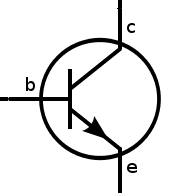
\includegraphics[scale=0.9]{0.cover.png}}
			%\caption{Caption}
			\label{fig:cover}
		\end{figure}
		
		\thispagestyle{empty} 
	\end{titlepage}
	
	\newpage
	\pagecolor{white}
	\section*{Prefazione}
	Organizzazione di eventuali risposte alle possibili domande esame all'orale di Elettronica.\\
	Notare che le risposte sono prese/ispirate dagli appunti, per ora sono un sempluce "copia e incolla", ma presto verranno rivisitate (ad ora risulteranno ripetitivi e poco utili).
	\tableofcontents
	\newpage
%************************************************************************************************************************************************************************************
	\section{Materiali semiconduttori}
	\subsection{Introduzione}
	Il corso di Fondamenti di Elettronica si occuperà principalmente dell’utilizzo dei dispositivi elettronici realizzati con i semiconduttori.\\
	La principale differenza rispetto a quanto visto nei corsi di Elettrotecnica, consiste nel fatto che i dispositivi elettronici non hanno una relazione lineare tra corrente e tensione.\\
	I circuiti realizzabili con i dispositivi elettronici sono suddivisibili in due gruppi:
	\begin{itemize}
		\item Analogici
		\item Digitali
	\end{itemize}
	In questo corso tratteremo solo i circuiti digitali lasciando la trattazione dettagliata dei circuiti analogici a corsi più specifici.\\
	Uno schema generico del corso in oggetto è riportato in Figura \ref{fig:im-1}.
	\begin{center}
		\begin{figure}[h]
			\centering
			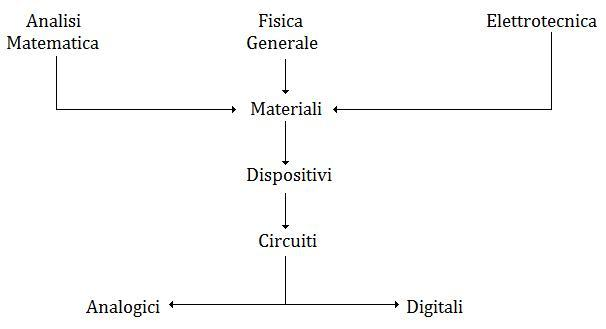
\includegraphics[scale=0.55]{1.png}
			\caption{Origini ed oggetto di studio del corso}
			\label{fig:im-1}
		\end{figure}
	\end{center}
	\subsection{Semiconduttori}
	\subsubsection{Premessa}
	Sappiamo che l’intensità di corrente ($J$) è legata al campo elettrico ($E$) dalla relazione:
	$$\vec{J} = \sigma \vec{E}$$
	Se la conducibilità ($\sigma$) è elevata, siamo in presenza di un \textbf{conduttore}; se $\sigma$ è ridotta siamo in presenza di un \textbf{isolante}.\\
	Possiamo dunque dire che i materiali \textbf{semiconduttori} sono materiali che si pongono a metà strada tra i conduttori (materiali ben disposti a condurre corrente sotto l’azione di un campo elettrico) e gli isolanti.\\\\
	La definizione appena data è però solo quantitativa. \\
	In realtà sappiamo che all’aumentare della temperatura, nei conduttori la conducibilità tende a diminuire mentre nei semiconduttori abbiamo il comportamento contrario: \textbf{all’aumento della temperatura, la conducibilità di un semiconduttore aumenta}.\\\\
	Dalla Fisica e dalla Chimica sappiamo inoltre che gli elettroni ruotano attorno al nucleo dell’atomo su un’orbita e con una velocità tali da controbilanciare esattamente la forza attrattiva del nucleo.\\
	Dall’orbita percorsa dall’elettrone possiamo allora associare ad ogni elettrone una energia (l’energia cinetica) ed una forza (la forza attrattiva del nucleo).\\
	In particolare, in un \textbf{sistema atomico}, sono permessi solo alcuni valori di energia (alcune orbite non sono cioè percorribili).\\
	Siccome gli elettroni hanno natura sia corpuscolare sia ondulatoria è anche necessario che al termine di un’orbita un elettrone abbia effettuato un multiplo intero di periodi ondulatori.
	\subsubsection{Conclusioni}
	Non tutti i valori energetici visualizzabili su un asse sono accessibili agli elettroni.\\
	In altre parole l’energia degli elettroni è quantizzata (principio di quantizzazione dell’energia).\\\\
	Ogni valore energetico consentito può essere assunto da uno ed un solo elettrone (principio di esclusione di \textbf{Pauli} \footnote{In realtà su ogni livello possono essere presenti fino a due elettroni caratterizzati da un momento di spin opposto.}).\\
	Dal principio di esclusione deduciamo che esistono livelli occupati e livelli liberi.\\
	In condizioni di quiete gli elettroni si posizionano spontaneamente sui livelli ad energia più bassa.\\
	È inoltre possibile determinare, tramite analisi statistiche, un livello energetico (detto livello energetico di \textbf{Fermi}, $E_F$) che discrimina tra i livelli completamente occupati ed i livelli liberi in condizione di quiete.
	\subsubsection{Sistemi Multiatomici}
	I livelli energetici rilevati nei sistemi monoatomici sono leggermente diversi dai livelli energetici rilevabili sui sistemi biatomici ma tutte le proprietà precedenti sono invariate. \\
	Avvicinando sempre più due atomi arriveremo alla fine a creare un legame tra i due detto legame covalente. \\
	Solitamente gli elettroni che formano il legame sono quelli con livelli energetici più elevati.\\\\
	Aumentando sempre più il numero degli atomi avremo fasce molto dense di livelli energetici distinti. \\
	Allora avremo una \textbf{struttura energetica a bande}. \\
	Una struttura energetica a bande è una struttura energetica in cui si alternano bande dense di livelli energetici permessi a bande proibite.\\\\
	Per muovere un elettrone allora sarà necessaria un’energia tale da spostarlo dal livello energetico in cui si trova ad un altro livello energetico permesso e libero. \\
	Allo zero assoluto l’elettrone al livello più prossimo al livello di Fermi sarà quello per il quale l’energia utilizzata sarà minima.\\\\
	Nei conduttori, il livello di Fermi è interno ad una banda permessa e, pertanto, per eccitare gli elettroni è necessaria poca energia.\\ 
	Negli isolanti, invece, il livello di Fermi è posto in una banda proibita e quindi è necessaria una grande quantità di energia per eccitare gli elettroni.\\\\
	Il semiconduttore ha dunque una struttura quantitativa uguale a quella di un isolante. \\
	La differenza è qualitativa: il gap tra due bande permesse è molto più piccolo rispetto allo stesso gap di un isolante.\\\\
	Sono semiconduttori quei materiali in cui, a temperatura ambiente, gli elettroni possono essere eccitati per il semplice effetto dello scambio termico con l’ambiente. \\
	Una volta eccitato l’elettrone si troverà in una zona con molti livelli energetici liberi in cui muoversi e condurre corrente.\\
	La Figura \ref{fig:im-2} mostra la struttura energetica di isolanti, semiconduttori e conduttori.
	\begin{center}
		\begin{figure}[h]
			\centering
			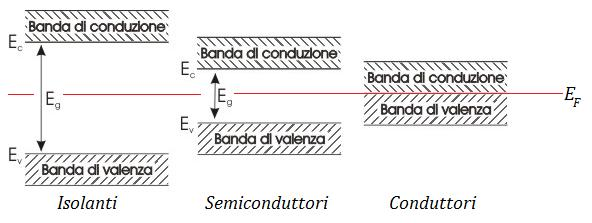
\includegraphics[scale=0.55]{2.png}
			\caption{Origini ed oggetto di studio del corso}
			\label{fig:im-2}
		\end{figure}
	\end{center}
	Un’altra differenza fondamentale è che a mano a mano che gli elettroni a livelli energetici più elevati si spostano ad energie superiori al livello di Fermi, i livelli da essi precedentemente occupati vengono via via liberati. \\
	Allora avremo due bande parzialmente occupate in cui sarà necessaria poca energia per eccitare altri elettroni.\\\\
	La tabella \hyperref[tab:table-1] riassume quanto appena visto.
	\begin{table}[ht]
		\centering
		\begin{tabular}{|l|c|c|c|}
			\hline
			& $E_F$ & Gap & Bande di conduzione \\ \hline
			\textbf{Conduttore} & Interno & Molto ridotto & Una \\ \hline
			\textbf{Semiconduttore} & Esterno & Ridotto & Due \\ \hline
			\textbf{Isolante} & Esterno & Elevato & Due \\ \hline
		\end{tabular}
		\caption{Caratteristiche principali dei conduttori, dei semiconduttori e degli isolanti}
		\label{tab:table-1}
	\end{table}
	La banda immediatamente superiore al livello di Fermi è detta \textbf{banda di conduzione} mentre la banda inferiore al livello di Fermi è detta è detta \textbf{banda di valenza}.\\\\
	I materiali semiconduttori sono tutti i materiali posti sulla quarta colonna della tavola periodica degli elementi. \\
	In particolare useremo il \textbf{Silicio (Si)} ed il \textbf{Germanio (Ge)} ed alcuni materiali composti quali l’arseniuro di gallio (GaAs) ed il fosfuro di indio (InP).
	\subsection{Il Silicio (Si)}
	Il silicio (simbolo Si; numero atomico 14) è un elemento della quarta colonna della tavola periodica degli elementi. \\
	La banda di valenza del silicio presenta quattro elettroni. \\
	Il silicio genera un reticolo cristallino cubico a facce centrate che è rappresentabile in due dimensioni come in Figura \ref{fig:im-3}.
	\begin{figure}[h]
		
		\begin{subfigure}{0.5\textwidth}
			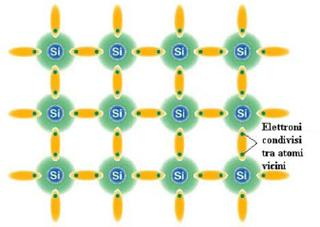
\includegraphics[width=0.9\linewidth, height=6cm]{3.png} 
			\caption{Reticolo cristallino del silicio sviluppato su due dimensioni}
			\label{fig:im-3}
		\end{subfigure}
		\begin{subfigure}{0.5\textwidth}
			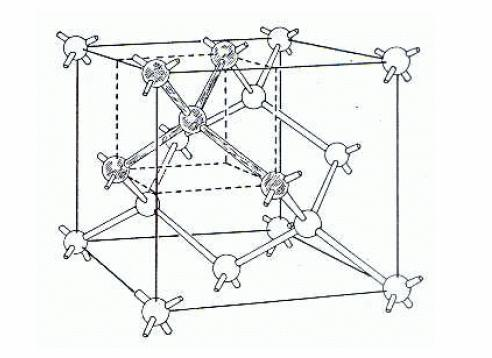
\includegraphics[width=0.9\linewidth, height=6cm]{4.png}
			\caption{Reticolo cristallino tridimensionale del silicio}
			\label{fig:im-4}
		\end{subfigure}
		
		\caption{}
		\label{fig:image1}
	\end{figure}
	In condizione di quiete la carica del cristallo di silicio è nulla in qualunque suo punto. \\
	Per tale motivo la densità locale di carica ($\rho$) è costante in qualsiasi punto del dispositivo.\\\\
	Quando il cristallo di silicio riceve energia sufficiente a consentire ad uno o più elettroni il salto dell’energy gap, il dispositivo resta globalmente neutro.\\\\
	Tuttavia a livello locale, in un punto del dispositivo avremo un elettrone in più mentre in un altro punto ne avremo uno in meno.\\\\
	A questo punto l’assenza di un elettrone in un punto del cristallo provoca una carica locale positiva. \\
	Questa carica positiva però attira a sé nuovi elettroni. \\
	Per compiere il salto da un livello occupato al livello liberato dal precedente elettrone serve un quantitativo di energia molto minore rispetto alla quantità necessaria per liberare il primo elettrone.\\\\
	Allora in un semiconduttore si hanno due meccanismi: una carica negativa si muove seguendo l’elettrone ed una carica positiva si muove seguendo l’assenza di un elettrone di legame. \\
	Poiché il trasporto di energia è dovuto a due portatori di carica di segno opposto, si parla di trasporto bipolare.\\\\
	Dal momento che la carica positiva è dovuta all’assenza di un elettrone si dice che essa è dovuta ad una lacuna (in inglese è detta hole, buco).
	\subsection{Elettroni e Lacune}
	Le lacune e gli elettroni vengono solitamente misurati in densità poiché è più importante conoscere quante lacune od elettroni vi sono in un volume. \\
	Indicheremo con $n$ il \textbf{numero di elettroni liberi }nella banda di conduzione per unità di volume (l’unità di misura sarà l’inverso di un volume); indicheremo invece con $p$ il \textbf{numero di lacune} nell’unità di volume.
	$$n = \frac{\text{elettroni liberi in conduzione}}{\text{volume } (cm^3)}$$
	$$p = \frac{\text{lacune}}{\text{volume } (cm^3)}$$
	Per quanto detto fino ad ora è evidente che gli elettroni e le lacune nascono contemporaneamente. \\
	Dal momento che esiste l’evento di generazione di elettrone e lacuna deve esistere, affinché il sistema rimanga stabile, anche un meccanismo contrario per il quale le coppie scompaiano. \\
	La scomparsa delle coppie avviene quando diminuendo la propria energia, l’elettrone trova una lacuna e vi si insedia.\\\\
	L’energia può essere ottenuta o ceduta in vari modi (tra i più comuni vi sono il calore, le radiazioni elettromagnetiche e la luce).\\\\
	Indichiamo con $G$ il tasso di generazione e con $R$ il tasso di ricombinazione.
	$$G = \frac{\text{coppie generate}}{\text{volume tempo } (cm^3 s)}$$
	$$R = \frac{\text{coppie ricombinate}}{\text{volume tempo } (cm^3 s)}$$
	In condizioni di stazionarietà deve essere $G = R$. \\
	Questa uguaglianza non indica che non vi siano coppie: significa semplicemente che per ogni coppia creata in un dato istante, una seconda coppia scompare.\\\\
	Possiamo inoltre vedere $p$ ed $n$ come funzione della temperatura:
	$$n = p = n_i(T) \implies p \cdot n = n_i^2$$
	Alla temperatura di riferimento di 300° Kelvin (circa 27° Celsius), abbiamo:
	$$n_i(300) \approx 10^{10} \text{ cm}^3$$
	Siccome in un centimetro cubo esistono circa $10^{23}$ atomi, la generazione di coppie interessa un atomo ogni $10^{13}$ atomi. \\
	Nonostante sia un valore così ridotto rispetto al numero totale di elettroni, esso è comunque sufficiente a far condurre il materiale.
	\subsection{Drogaggi}
	Fino ad ora abbiamo visto che in un materiale puro (intrinseco), deve necessariamente essere verificata l’uguaglianza $n = p$.\\
	È però possibile spezzare il vincolo appena enunciato modificando la struttura del reticolo cristallino inserendovi, senza alterare la struttura del silicio\footnote{Modificando la struttura del cristallo avremmo una lega.}, elementi della terza o della quinta colonna della tavola periodica.\\
	Questa operazione prende il nome di \textbf{drogaggio}. \\
	Nel drogaggio si usano soprattutto il Fosforo (simbolo P; numero atomico 15) ed il Boro (simbolo B; numero atomico 5).
	\begin{figure}[h]
		
		\begin{subfigure}{0.5\textwidth}
			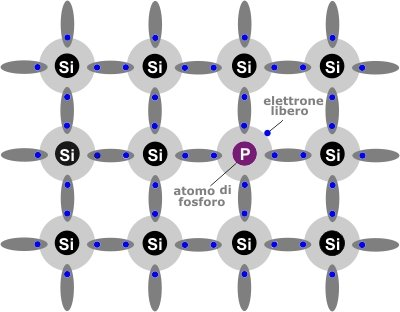
\includegraphics[width=0.9\linewidth, height=6cm]{5.png} 
			\caption{Reticolo cristallino del silicio drogato con atomi di fosforo}
			\label{fig:im-5}
		\end{subfigure}
		\begin{subfigure}{0.5\textwidth}
			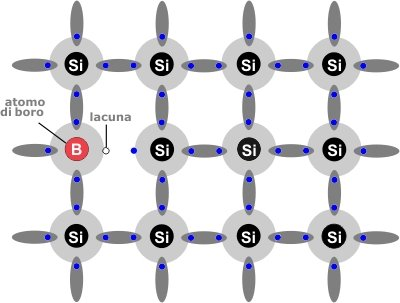
\includegraphics[width=0.9\linewidth, height=6cm]{6.png}
			\caption{Reticolo cristallino del silicio drogato con atomi di boro}
			\label{fig:im-6}
		\end{subfigure}
		
		\caption{}
		\label{fig:image2}
	\end{figure}
	Usando un atomo di fosforo (elemento della quinta colonna) abbiamo un elettrone che non si lega con altri atomi. \\
	L’elettrone libero è ora bilanciato da una carica positiva fissa (il protone del fosforo non si muove). \\
	Allora la lacuna fissa non fornisce contributo alle correnti e quindi non è più vero che $p = n$.\\\\
	Poiché il fosforo dona il suo elettrone di legame inutilizzato, viene detto donatore. \\
	Indicheremo allora con $N_D$ il numero di atomi donatori. \\
	Concentrazioni tipiche arrivano fino a $10^{21}$ per centimetro cubo (e siccome la densità del reticolo di silicio è pari a $10^{23}$ significa che un atomo ogni cento porta carica).\\\\
	Si faccia inoltre attenzione al fatto che i livelli proibiti al silicio non sono proibiti al fosforo. \\
	Allora abbiamo un nuovo livello energetico, prima proibito, vicino alla banda di conduzione, utilizzabile dagli atomi.\\\\
	Un materiale drogato viene detto \textbf{estrinseco}.\\\\
	Usando materiali della \textbf{quinta colonna} abbiamo uno sbilanciamento in favore degli elettroni ($n > p$).\\\\
	Usando invece materiali della \textbf{terza colonna} provochiamo uno sbilanciamento in favore delle lacune ($n < p$) poiché abbiamo uno spostamento della lacuna dovuta all’assenza di un elettrone nell’atomo usato per il drogaggio. \\
	In questo caso generiamo una lacuna mobile senza generare un elettrone mobile. \\
	Gli atomi della terza colonna sono capaci di accettare un elettrone di legame senza mettere a disposizione una lacuna mobile e sono pertanto detti accettori. \\
	Indicheremo allora con $N_A$ il numero di atomi accettori. \\
	In questo caso generiamo un nuovo livello energetico vicino alla banda di valenza.
	\subsection{Problemi}
	Nasce ora un problema: come dipendono $p$ ed $n$ dalla temperatura? \\
	Per i materiali estrinseci non è più vera l’uguaglianza:
	$$p = n = n_i(T)$$
	dal momento che $p \neq n$.\\
	Resta tuttavia vero che:
	$$p \cdot n = n_i^2(T)$$
	Inoltre è vero che $R$ e $G$ restano equivalenti. \\
	Siccome $G$ dipende solo dalla temperatura e $R$ dipende dalla temperatura e dal numero di elettroni e lacune in circolazione.
	$$G = g(T)$$
	$$R = p \cdot n \cdot f(T)$$
	Allora per l’equilibrio abbiamo:
	$$g(T) = n \cdot p \cdot f(T) \implies p \cdot n = \frac{g(T)}{f(T)} = z(T)$$
	Dunque, noto il valore di $p \cdot n$ in una situazione, possiamo ricavarne il valore per qualsiasi condizione.\\\\
	Il dispositivo deve inoltre essere globalmente neutro. \\
	La densità di carica è data da:
	$$\rho = \underbrace{(-qn)}_{\text{dovuta agli elettroni}} + \underbrace{(+qp)}_{\text{dovuta ai protoni}} + \underbrace{(+qN_D)}_{\text{atomi donatori}} + \underbrace{(-qN_A)}_{\text{atomi accettori}}$$
	Raccogliendo ed imponendo la densità pari a zero, abbiamo:
	$$\rho = q \left( \underbrace{N_D - N_A}_{\text{cariche fisse}} + \underbrace{p - n}_{\text{cariche mobili}} \right) = 0$$
	Dal momento che sappiamo essere:
	$$p = \frac{n_i^2}{n}$$
	abbiamo una equazione in una incognita:
	$$\rho = q\left(N_D - N_A + \frac{n_i^2}{n} - n\right) = 0 \implies n^2 - (N_D - N_A)n - n_i^2 = 0$$
	da cui possiamo ottenere facilmente il valore di $n$.
	$$n = \frac{(N_D - N_A) + \sqrt{(N_D - N_A)^2 + 4n_i^2}}{2}$$
	possiamo facilmente ricavare la densità di carica in un materiale estrinseco uniformemente drogato.
	\subsection{Proprietà}
	\subsubsection{Principio di compensazione}
	Il calcolo del valore di $n$ (che è una grandezza fisica necessariamente positiva) può essere molto semplificato nel caso in cui sia $N_D \gg N_A$.
	$$n \approx \frac{N_D + \sqrt{N_D^2}}{2} \approx N_D \implies p = \frac{n_i^2}{N_D}$$
	Quesrto risultato dimostra che è possibile decidere il numero di elettroni liberi drogando in modo opportuno il materiale. \\
	Casi tipici sono i seguenti:
	$$\begin{aligned} N_D &= 10^{15} cm^{-3} \\ n_i &= 10^{10} cm^{-3} \end{aligned} \implies \begin{aligned} n &= 10^{15} cm^{-3} \\ p &= 10^5 cm^{-3} \end{aligned}$$
	Una regione così drogata è detta regione estrinseca di tipo $n$.\\\\
	Nel caso in cui sia $N_A \gg N_D$, ripedendo gli stessi calcoli appena effettuati, avremo una regione estrinseca di tipo $p$.\\\\
	Si noti che il valore di $p$ viene ricavato per differenza. \\
	Allora drogando con concentrazioni identiche di atomi accettori e donatori è come se il materiale non fosse stato drogato (l’elettrone libero donato dal donatore viene catturato dall’accettore e la coppia elettrone lacuna scompare). \\
	Questa proprietà è detta \textbf{principio di compensazione}.
	\subsubsection{Legge di Ohm}
	Sappiamo che i materiali conduttori rispettano la legge di Ohm per cui vale:
	$$\vec{J} = \sigma \vec{E}$$
	Questa relazione vale anche per i semiconduttori?\\\\
	Per rispondere a questa domanda consideriamo un dispositivo bidimensionale uniformemente drogato con $N_D \gg N_A$ atomi donatori. \\
	Applichiamo ad esse un campo elettrico $\vec{E}$.\\\\
	La forza esercitata dal campo su una singola carica $q$ è:
	$$f = -qE$$
	e siccome vale sempre $f = ma$, abbiamo:
	$$ma = -qE \implies \vec{a} = \frac{-q}{m} \vec{E}$$
	che porta ad un moto uniformemente accelerato.\\\\
	Questo risultato è però valido solo nel vuoto. \\
	In realtà l’elettrone si muove all’interno di un reticolo di protoni, neutroni ed elettroni che i quali interagisce. \\
	A causa di tutte le interazioni dell’elettrone con il reticolo, possiamo dire che esso si muove mediamente nella direzione opposta a quella del campo elettrico. \\
	Sperimentalmente si vede che l’elettrone si muove con una velocità mediamente costante e proporzionale al campo elettrico detta mobilità elettronica ed indicata con $\mu_n$.
	$$\vec{v}_n = -\mu_n \vec{E}$$
	Ragionando in modo analogo possiamo arrivare ad un risultato simile per le lacune:
	$$\vec{v}_p = +\mu_p \vec{E}$$
	Contrariamente agli elettroni le lacune si muovono però nel verso del campo elettrico. \\
	Inoltre si ha che la mobilità delle lacune $\mu_p$ è tipicamente inferiore alla mobilità degli elettroni.\\\\
	L’intensità della corrente è data da:
	$$J = \frac{I}{s}$$
	dove vale:
	$$I = \frac{dQ}{dt}$$
	dove $dQ$ è la carica di un cilindro di base $s$ ed altezza $dx$.
	$$dQ = -q \cdot n \cdot s \cdot dx$$
	Siccome è:
	$$dx = -v_n dt$$
	e poiché è $v_n = -\mu_n E$, raggruppando tutti i risultati ottenuti abbiamo:
	$$J_n = \frac{(-q)ns(-\mu_n)E \, dt}{s \, dt} = q\mu_n nE = q\mu_n N_D E$$
	dove abbiamo sfruttato il fatto che $n = N_D$ per il fatto che possiamo controllare il drogaggio del materiale. \\
	Definendo ora
	$$\sigma_n = q\mu_n N_D$$
	otteniamo la \textbf{legge di Ohm in forma locale}:
	$$J_n = \sigma_n E$$
	Per le lacune vale invece:
	$$\sigma_p = q\mu_p p \implies J_p = \sigma_p E$$
	In forma più generale abbiamo:
	$$J = J_n + J_p = q(\mu_n n + \mu_p p)E$$
	Poiché il valore di $\sigma$ dipende dal drogaggio che si è utilizzato, possiamo realizzare, drogando opportunamente le varie porzioni del dispositivo, parti fortemente conduttive e parti fortemente resistive. \\
	Su un unico semiconduttore possiamo quindi costruire sia i dispositivi sia le connessioni tra i dispositivi.
	\subsection{Drogaggi Non Uniformi}
	Fino ad ora abbiamo considerato solo materiali \textbf{uniformemente drogati}. \\
	Per quanto appena detto è però necessario considerare che il materiale possa non essere uniformemente drogato. \\
	Nuovamente poniamoci nel caso bidimensionale all’equilibrio in cui la concentrazione varia linearmente con $x$.\\\\
	All’equilibrio non vi è energia che circola. \\
	Siccome gli elettroni in movimento dissipano energia deve essere:
	$$J = J_n = J_p = 0$$
	Gli elettroni tuttavia scambiano energia tra di loro con bilanci mediamente nulli. \\
	Questo non vuol dire che l’elettrone sia fermo: significa solamente che la probabilità che ha un elettrone di muoversi con velocità termica $v_{th}(T)$ è pari alla probabilità che esso ha di muoversi con velocità $-v_{th}(T)$.\\\\
	Allora in questo caso abbiamo due volumetti interessati dal movimento. \\
	Entrambi i volumetti sono di dimensione $sdx$ dove si ha $dx = v_{th} \, dt$.\\\\
	Nuovamente abbiamo:
	$$J = \frac{I}{s}$$
	$$I = \frac{dQ}{dt}$$
	Questa volta avremo però:
	$$dQ = \frac{dQ_1}{2} - \frac{dQ_2}{2}$$
	dove
	$$dQ_1 = (-q) n_1 \cdot s dx$$
	$$dQ_2 = (-q) n_2 \cdot s dx$$
	in cui $n_1 \neq n_2$ sono i valori medi della densità di carica nelle sezioni limitrofe al valore di riferimento.\\\\
	Sfruttando i valori di $dQ_1$ e $dQ_2$ e l’espressione di $J$ abbiamo ora:
	$$J = \frac{-qn_1 sv_{th} dt + qn_2 sv_{th} dt}{2s dt} = \frac{q}{2}(n_2 - n_1)v_{th}$$
	\textbf{che è in contrasto con l’ipotesi di equilibrio da cui siamo partiti}.\\\\
	In realtà, siccome le concentrazioni non sono uniformi, gli elettroni tendono a diffondersi dalle regioni a densità maggiore a quelle a densità minore. \\
	Ciò è detto principio di diffusione ed è simile a quanto avviene lasciando cadere una goccia di inchiostro in un bicchiere d’acqua.\\\\
	In altre parole, per effetto termico, gli elettroni tendono ad appiattire la curva della concentrazione.\\\\
	L’elettrone si può dunque muovere per due motivi: o per l’effetto di un campo elettrico o per effetto diffusivo. \\
	Nel caso di un drogaggio non uniforme, entrambi questi effetti sono rilevanti.\\\\
	Allora in un semiconduttore abbiamo due meccanismi di spostamento mentre in un conduttore vi è solo l’azione del campo elettrico.\\\\
	La corrente di diffusione degli elettroni è dunque data da:
	$$J_n = q D_n \frac{dn}{dx}$$
	dove $D_n$ è il \textbf{coefficiente di diffusione} e dipende grandemente dalla temperatura. \\
	In particolare vale la \textbf{Relazione di Einstein}:
	$$D_n = \frac{KT}{q} \mu_n$$
	dove $K = 1,38 \cdot 10^{-23}$ è la \textbf{costante di Boltzman}.\\\\
	Ragionando nello stesso modo per le lacune otteniamo la versione analoga per le lacune:
	$$J_p = -q D_p \frac{dp}{dx}$$
	$$D_p = \frac{KT}{q} \mu_p$$
	È ormai evidente che \textbf{è difficile ottenere un moto puramente diffusivo} poiché nel momento in cui un elettrone si muove, si viene a creare un dipolo che genera un campo elettrico. \\
	Applicando allora una versione semplificata del principio di sovrapposizione degli effetti possiamo ottenere un modello complessivo.
	$$J = J_n + J_p = 0$$
	$$J_n = -q \mu_n n E + q D_n \frac{dn}{dx}$$
	$$J_p = q \mu_p p E - q D_p \frac{dp}{dx}$$
	Nel caso multidimensionale sarà:
	$$J_n = -q \mu_n n E + q D_n \text{grad}(n)$$
	$$J_p = q \mu_p p E + q D_p \text{grad}(p)$$
	Questo modello è detto \textbf{modello a trascinamento diffusivo} (drift diffusion in inglese) e \textbf{sostituisce la legge di Ohm per lo studio dei semiconduttori}.
	\subsection{Relazioni}
	Per i semiconduttori abbiamo quindi le relazioni seguenti:
	$$E = -\frac{dQ}{dx}$$
	$$\rho = q(N_D - N_A + p - n)$$
	$$\frac{d(\varepsilon E)}{dx} = \underbrace{\rho}_{\text{Densità di carica}}$$
	$$J = J_n + J_p = 0$$
	$$J_n = -q\mu_n n E + qD_n \frac{dn}{dx}$$
	$$J_p = q\mu_p p E - qD_p \frac{dp}{dx}$$
%************************************************************************************************************************************************************************************
	\section{Conduzione elettrica in un materiale semiconduttore uniforme}
	\subsection{Semiconduttori}
	\subsubsection{Premessa}
	Sappiamo che l’intensità di corrente ($J$) è legata al campo elettrico ($E$) dalla relazione:
	$$\vec{J} = \sigma \vec{E}$$
	Se la conducibilità ($\sigma$) è elevata, siamo in presenza di un \textbf{conduttore}; se $\sigma$ è ridotta siamo in presenza di un \textbf{isolante}.\\
	Possiamo dunque dire che i materiali \textbf{semiconduttori} sono materiali che si pongono a metà strada tra i conduttori (materiali ben disposti a condurre corrente sotto l’azione di un campo elettrico) e gli isolanti.\\\\
	La definizione appena data è però solo quantitativa. \\
	In realtà sappiamo che all’aumentare della temperatura, nei conduttori la conducibilità tende a diminuire mentre nei semiconduttori abbiamo il comportamento contrario: \textbf{all’aumento della temperatura, la conducibilità di un semiconduttore aumenta}.\\\\
	Dalla Fisica e dalla Chimica sappiamo inoltre che gli elettroni ruotano attorno al nucleo dell’atomo su un’orbita e con una velocità tali da controbilanciare esattamente la forza attrattiva del nucleo.\\
	Dall’orbita percorsa dall’elettrone possiamo allora associare ad ogni elettrone una energia (l’energia cinetica) ed una forza (la forza attrattiva del nucleo).\\
	In particolare, in un \textbf{sistema atomico}, sono permessi solo alcuni valori di energia (alcune orbite non sono cioè percorribili).\\
	Siccome gli elettroni hanno natura sia corpuscolare sia ondulatoria è anche necessario che al termine di un’orbita un elettrone abbia effettuato un multiplo intero di periodi ondulatori.
	\subsubsection{Conclusioni}
	Non tutti i valori energetici visualizzabili su un asse sono accessibili agli elettroni.\\
	In altre parole l’energia degli elettroni è quantizzata (principio di quantizzazione dell’energia).\\\\
	Ogni valore energetico consentito può essere assunto da uno ed un solo elettrone (principio di esclusione di \textbf{Pauli} \footnote{In realtà su ogni livello possono essere presenti fino a due elettroni caratterizzati da un momento di spin opposto.}).\\
	Dal principio di esclusione deduciamo che esistono livelli occupati e livelli liberi.\\
	In condizioni di quiete gli elettroni si posizionano spontaneamente sui livelli ad energia più bassa.\\
	È inoltre possibile determinare, tramite analisi statistiche, un livello energetico (detto livello energetico di \textbf{Fermi}, $E_F$) che discrimina tra i livelli completamente occupati ed i livelli liberi in condizione di quiete.
	\subsubsection{Sistemi Multiatomici}
	I livelli energetici rilevati nei sistemi monoatomici sono leggermente diversi dai livelli energetici rilevabili sui sistemi biatomici ma tutte le proprietà precedenti sono invariate. \\
	Avvicinando sempre più due atomi arriveremo alla fine a creare un legame tra i due detto legame covalente. \\
	Solitamente gli elettroni che formano il legame sono quelli con livelli energetici più elevati.\\\\
	Aumentando sempre più il numero degli atomi avremo fasce molto dense di livelli energetici distinti. \\
	Allora avremo una \textbf{struttura energetica a bande}. \\
	Una struttura energetica a bande è una struttura energetica in cui si alternano bande dense di livelli energetici permessi a bande proibite.\\\\
	Per muovere un elettrone allora sarà necessaria un’energia tale da spostarlo dal livello energetico in cui si trova ad un altro livello energetico permesso e libero. \\
	Allo zero assoluto l’elettrone al livello più prossimo al livello di Fermi sarà quello per il quale l’energia utilizzata sarà minima.\\\\
	Nei conduttori, il livello di Fermi è interno ad una banda permessa e, pertanto, per eccitare gli elettroni è necessaria poca energia.\\ 
	Negli isolanti, invece, il livello di Fermi è posto in una banda proibita e quindi è necessaria una grande quantità di energia per eccitare gli elettroni.\\\\
	Il semiconduttore ha dunque una struttura quantitativa uguale a quella di un isolante. \\
	La differenza è qualitativa: il gap tra due bande permesse è molto più piccolo rispetto allo stesso gap di un isolante.\\\\
	Sono semiconduttori quei materiali in cui, a temperatura ambiente, gli elettroni possono essere eccitati per il semplice effetto dello scambio termico con l’ambiente. \\
	Una volta eccitato l’elettrone si troverà in una zona con molti livelli energetici liberi in cui muoversi e condurre corrente.\\
	La Figura \ref{fig:im-2b} mostra la struttura energetica di isolanti, semiconduttori e conduttori.
	\begin{center}
		\begin{figure}[h]
			\centering
			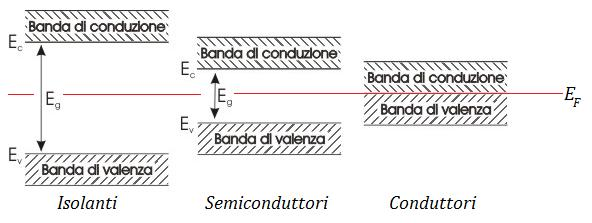
\includegraphics[scale=0.55]{2.png}
			\caption{Origini ed oggetto di studio del corso}
			\label{fig:im-2b}
		\end{figure}
	\end{center}
	Un’altra differenza fondamentale è che a mano a mano che gli elettroni a livelli energetici più elevati si spostano ad energie superiori al livello di Fermi, i livelli da essi precedentemente occupati vengono via via liberati. \\
	Allora avremo due bande parzialmente occupate in cui sarà necessaria poca energia per eccitare altri elettroni.\\\\
	La tabella \hyperref[tab:table-1b] riassume quanto appena visto.
	\begin{table}[ht]
		\centering
		\begin{tabular}{|l|c|c|c|}
			\hline
			& $E_F$ & Gap & Bande di conduzione \\ \hline
			\textbf{Conduttore} & Interno & Molto ridotto & Una \\ \hline
			\textbf{Semiconduttore} & Esterno & Ridotto & Due \\ \hline
			\textbf{Isolante} & Esterno & Elevato & Due \\ \hline
		\end{tabular}
		\caption{Caratteristiche principali dei conduttori, dei semiconduttori e degli isolanti}
		\label{tab:table-1b}
	\end{table}
	La banda immediatamente superiore al livello di Fermi è detta \textbf{banda di conduzione} mentre la banda inferiore al livello di Fermi è detta è detta \textbf{banda di valenza}.\\\\
	I materiali semiconduttori sono tutti i materiali posti sulla quarta colonna della tavola periodica degli elementi. \\
	In particolare useremo il \textbf{Silicio (Si)} ed il \textbf{Germanio (Ge)} ed alcuni materiali composti quali l’arseniuro di gallio (GaAs) ed il fosfuro di indio (InP).
	\subsection{Proprietà}
	\subsubsection{Legge di Ohm}
	Sappiamo che i materiali conduttori rispettano la legge di Ohm per cui vale:
	$$\vec{J} = \sigma \vec{E}$$
	Questa relazione vale anche per i semiconduttori?\\\\
	Per rispondere a questa domanda consideriamo un dispositivo bidimensionale uniformemente drogato con $N_D \gg N_A$ atomi donatori. \\
	Applichiamo ad esse un campo elettrico $\vec{E}$.\\\\
	La forza esercitata dal campo su una singola carica $q$ è:
	$$f = -qE$$
	e siccome vale sempre $f = ma$, abbiamo:
	$$ma = -qE \implies \vec{a} = \frac{-q}{m} \vec{E}$$
	che porta ad un moto uniformemente accelerato.\\\\
	Questo risultato è però valido solo nel vuoto. \\
	In realtà l’elettrone si muove all’interno di un reticolo di protoni, neutroni ed elettroni che i quali interagisce. \\
	A causa di tutte le interazioni dell’elettrone con il reticolo, possiamo dire che esso si muove mediamente nella direzione opposta a quella del campo elettrico. \\
	Sperimentalmente si vede che l’elettrone si muove con una velocità mediamente costante e proporzionale al campo elettrico detta mobilità elettronica ed indicata con $\mu_n$.
	$$\vec{v}_n = -\mu_n \vec{E}$$
	Ragionando in modo analogo possiamo arrivare ad un risultato simile per le lacune:
	$$\vec{v}_p = +\mu_p \vec{E}$$
	Contrariamente agli elettroni le lacune si muovono però nel verso del campo elettrico. \\
	Inoltre si ha che la mobilità delle lacune $\mu_p$ è tipicamente inferiore alla mobilità degli elettroni.\\\\
	L’intensità della corrente è data da:
	$$J = \frac{I}{s}$$
	dove vale:
	$$I = \frac{dQ}{dt}$$
	dove $dQ$ è la carica di un cilindro di base $s$ ed altezza $dx$.
	$$dQ = -q \cdot n \cdot s \cdot dx$$
	Siccome è:
	$$dx = -v_n dt$$
	e poiché è $v_n = -\mu_n E$, raggruppando tutti i risultati ottenuti abbiamo:
	$$J_n = \frac{(-q)ns(-\mu_n)E \, dt}{s \, dt} = q\mu_n nE = q\mu_n N_D E$$
	dove abbiamo sfruttato il fatto che $n = N_D$ per il fatto che possiamo controllare il drogaggio del materiale. \\
	Definendo ora
	$$\sigma_n = q\mu_n N_D$$
	otteniamo la \textbf{legge di Ohm in forma locale}:
	$$J_n = \sigma_n E$$
	Per le lacune vale invece:
	$$\sigma_p = q\mu_p p \implies J_p = \sigma_p E$$
	In forma più generale abbiamo:
	$$J = J_n + J_p = q(\mu_n n + \mu_p p)E$$
	Poiché il valore di $\sigma$ dipende dal drogaggio che si è utilizzato, possiamo realizzare, drogando opportunamente le varie porzioni del dispositivo, parti fortemente conduttive e parti fortemente resistive. \\
	Su un unico semiconduttore possiamo quindi costruire sia i dispositivi sia le connessioni tra i dispositivi.
%************************************************************************************************************************************************************************************
	\section{Diffusione termica}
	\subsection{Drogaggi Non Uniformi}
	Fino ad ora abbiamo considerato solo materiali \textbf{uniformemente drogati}. \\
	Per quanto appena detto è però necessario considerare che il materiale possa non essere uniformemente drogato. \\
	Nuovamente poniamoci nel caso bidimensionale all’equilibrio in cui la concentrazione varia linearmente con $x$.\\\\
	All’equilibrio non vi è energia che circola. \\
	Siccome gli elettroni in movimento dissipano energia deve essere:
	$$J = J_n = J_p = 0$$
	Gli elettroni tuttavia scambiano energia tra di loro con bilanci mediamente nulli. \\
	Questo non vuol dire che l’elettrone sia fermo: significa solamente che la probabilità che ha un elettrone di muoversi con velocità termica $v_{th}(T)$ è pari alla probabilità che esso ha di muoversi con velocità $-v_{th}(T)$.\\\\
	Allora in questo caso abbiamo due volumetti interessati dal movimento. \\
	Entrambi i volumetti sono di dimensione $sdx$ dove si ha $dx = v_{th} \, dt$.\\\\
	Nuovamente abbiamo:
	$$J = \frac{I}{s}$$
	$$I = \frac{dQ}{dt}$$
	Questa volta avremo però:
	$$dQ = \frac{dQ_1}{2} - \frac{dQ_2}{2}$$
	dove
	$$dQ_1 = (-q) n_1 \cdot s dx$$
	$$dQ_2 = (-q) n_2 \cdot s dx$$
	in cui $n_1 \neq n_2$ sono i valori medi della densità di carica nelle sezioni limitrofe al valore di riferimento.\\\\
	Sfruttando i valori di $dQ_1$ e $dQ_2$ e l’espressione di $J$ abbiamo ora:
	$$J = \frac{-qn_1 sv_{th} dt + qn_2 sv_{th} dt}{2s dt} = \frac{q}{2}(n_2 - n_1)v_{th}$$
	\textbf{che è in contrasto con l’ipotesi di equilibrio da cui siamo partiti}.\\\\
	In realtà, siccome le concentrazioni non sono uniformi, gli elettroni tendono a diffondersi dalle regioni a densità maggiore a quelle a densità minore. \\
	Ciò è detto \textbf{principio di diffusione (termica)} ed è simile a quanto avviene lasciando cadere una goccia di inchiostro in un bicchiere d’acqua.\\\\
	In altre parole, per effetto termico, gli elettroni tendono ad appiattire la curva della concentrazione.\\\\
	L’elettrone si può dunque muovere per due motivi: o per l’effetto di un campo elettrico o per effetto diffusivo. \\
	Nel caso di un drogaggio non uniforme, entrambi questi effetti sono rilevanti.\\\\
	Allora in un semiconduttore abbiamo due meccanismi di spostamento mentre in un conduttore vi è solo l’azione del campo elettrico.\\\\
	La corrente di diffusione degli elettroni è dunque data da:
	$$J_n = q D_n \frac{dn}{dx}$$
	dove $D_n$ è il \textbf{coefficiente di diffusione} e dipende grandemente dalla temperatura. \\
	In particolare vale la \textbf{Relazione di Einstein}:
	$$D_n = \frac{KT}{q} \mu_n$$
	dove $K = 1,38 \cdot 10^{-23}$ è la \textbf{costante di Boltzman}.\\\\
	Ragionando nello stesso modo per le lacune otteniamo la versione analoga per le lacune:
	$$J_p = -q D_p \frac{dp}{dx}$$
	$$D_p = \frac{KT}{q} \mu_p$$
	È ormai evidente che \textbf{è difficile ottenere un moto puramente diffusivo} poiché nel momento in cui un elettrone si muove, si viene a creare un dipolo che genera un campo elettrico. \\
	Applicando allora una versione semplificata del principio di sovrapposizione degli effetti possiamo ottenere un modello complessivo.
	$$J = J_n + J_p = 0$$
	$$J_n = -q \mu_n n E + q D_n \frac{dn}{dx}$$
	$$J_p = q \mu_p p E - q D_p \frac{dp}{dx}$$
	Nel caso multidimensionale sarà:
	$$J_n = -q \mu_n n E + q D_n \text{grad}(n)$$
	$$J_p = q \mu_p p E + q D_p \text{grad}(p)$$
	Questo modello è detto \textbf{modello a trascinamento diffusivo} detto anche \textbf{modello Ohmico-Diffusivo} (\textbf{drift diffusion model} in inglese) e \textbf{sostituisce la legge di Ohm per lo studio dei semiconduttori}.
%************************************************************************************************************************************************************************************
	\section{Modello di trasporto ohmico-diffusivo}
	\textbf{N.B}: Parte di questa risposta va presa dalla risposta precedente.\\\\
	Si può quindi introdurre la (seconda) differenza tra materiali semi-conduttori e conduttori: in un materiale semi-conduttore non uniformemente drogato non vale più la legge di Ohm, perché bisogna tener conto di una componente di corrente diffusiva, oltre alla componente ohmica tipica dei conduttori.\\\\
	Quindi, per un materiale semi-conduttore non uniformemente drogato, si utilizza un modello ohmico-diffusivo ("drift-diffusion model"):
	$$j_n = j_{n,E} + j_{n,diff} = \underbrace{q\mu_n n E}_{\text{comp. ohmica}} + \underbrace{q D_n \frac{dn}{dx}}_{\text{comp. diffusiva}}$$
	Lo stesso discorso si può fare per un materiale semi-conduttore non uniformemente drogato con atomi accettori, in condizione di equilibrio:
	$$j_p = j_{p,E} + j_{p,diff} = \underbrace{q\mu_p p E}_{\text{comp. ohmica}} - \underbrace{q D_p \frac{dp}{dx}}_{\text{comp. diffusiva}}$$
	Riassumendo, per un conduttore si ha un solo portatore di carica (gli elettroni) ed un solo meccanismo di trasporto (quello ohmico, dovuto al campo elettrico):
	$$j_{cond} = \sigma E$$
	mentre per un semi-conduttore si hanno due portatori di carica (gli elettroni e le lacune) e due meccanismi di trasporto (quello ohmico e quello diffusivo):
	$$j_{semic} = j_n + j_p = j_{n,E} + j_{n,diff} + j_{p,E} + j_{p,diff}$$
	Si consideri un materiale semiconduttore non uniformemente drogato e in condizione d'equilibrio.\\
	Siccome si è in condizione di equilibrio, nessuno sta fornendo energia al sistema e la corrente è nulla:
	$$j = j_n + j_p = 0 \quad \Rightarrow \quad j_n = j_p = 0$$
	Siccome la concentrazione non è uniforme, questo significa che dati due punti $x_1$ e $x_2$, $n(x_1) \neq n(x_2)$.
	\begin{center}
		\begin{figure}[h]
			\centering
			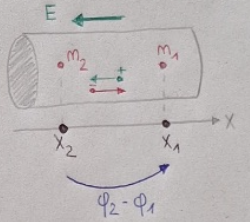
\includegraphics[scale=0.55]{a.png}
			\caption{}
			\label{fig:im-a}
		\end{figure}
	\end{center}
	Di conseguenza:
	$$j_n = q\mu_n n E + q D_n \frac{dn}{dx} = 0$$
	Ricordando che:
	$$E = -\frac{d\varphi}{dx} \quad \text{dove } \varphi \text{ è il potenziale}$$
	$$D_n = \frac{kT}{q} \mu_n$$
	segue che:
	$$-q\mu_n n \frac{d\varphi}{dx} + q \frac{kT}{q} \mu_n \frac{dn}{dx} = 0$$
	$$\frac{d\varphi}{dx} = \frac{kT}{q} \frac{1}{n} \frac{dn}{dx}$$
	Integrando da $x_1$ a $x_2$:
	$$\int_{x_1}^{x_2} \frac{d\varphi}{dx} dx = \int_{x_1}^{x_2} \frac{kT}{q} \frac{1}{n} \frac{dn}{dx} dx$$
	$$\Updownarrow$$
	$$\int_{\varphi_1 = \varphi(x_1)}^{\varphi_2 = \varphi(x_2)} d\varphi = \frac{kT}{q} \int_{n_1 = n(x_1)}^{n_2 = n(x_2)} \frac{1}{n} dn$$
	$$\Updownarrow$$
	$$\varphi_2 - \varphi_1 = \frac{kT}{q} \ln \left( \frac{n_2}{n_1} \right)$$
	Se $n_2 > n_1$, allora $\varphi_2 - \varphi_1 > 0$, ovvero si ha una differenza di potenziale, è quindi un campo elettrico che bilancia la componente diffusiva (perché il materiale non è uniforme).\\
	Più genericamente, stabilendo una coordinata $x_0$ di riferimento in cui $\varphi_0 = \varphi(x_0) = 0$ e $n(x_0) = n_0$, si può affermare che in condizione d'equilibrio il potenziale, in qualunque punto del materiale, è legato alla concentrazione di elettroni in tale punto dalla relazione:
	$$\varphi(x) = \frac{kT}{q} \ln \left[ \frac{n(x)}{n_0} \right] \quad \Leftrightarrow \quad n(x) = n_0 e^{\frac{q\varphi(x)}{kT}}$$
	Quindi, ad una lieve variazione del potenziale $\varphi(x)$, corrisponde una grande variazione della concentrazione $n(x)$. Il termine $\frac{kT}{q}$ è una tensione detta tensione termica:
	$$V_T = \frac{kT}{q}$$
	che, alla temperatura ambiente di 300 K, vale $V_T \approx 25$ mV.
	Dunque, si può riscrivere la relazione precedente come:
	$$\varphi(x) = V_T \ln \left[ \frac{n(x)}{n_0} \right] \quad \Leftrightarrow \quad n(x) = n_0 e^{\frac{q(x)}{V_T}}$$
	Analogamente, per le lacune, seguendo lo stesso ragionamento degli elettroni per $j_p$ e $D_p$, si ottiene un risultato simile:
	$$\varphi(x) = -V_T \ln \left[ \frac{p(x)}{p_0} \right] \quad \Leftrightarrow \quad p(x) = p_0 e^{\frac{-q(x)}{V_T}}$$
	Quindi, in un semiconduttore in condizione d'equilibrio, $p$, $n$ e $q$ sono strettamente legate fra loro (si ricorda che, in equilibrio, $pn = n_i^2$).
%************************************************************************************************************************************************************************************
	\section{Relazione fra potenziale elettrico e concentrazioni di portatori all'equilibrio}
	\subsection{Ricapitolando}
	Neila scorsa sezione abbiamo introdotto i semiconduttori e ne abbiamo evidenziato le principali differenze rispetto ai conduttori.\\\\
	Abbiamo inoltre modellizzato i semiconduttori come:
	$$\overline{J} = \overline{J}_n + \overline{J}_p$$
	dove $\overline{J}_n$ è la densità di corrente dovuta agli elettroni e $\overline{J}_p$ è la densità di corrente dovuta alle lacune. \\
	Nel casobidimensionale (che è il caso di nostro interesse), tali componenti si possono esprimere come:
	$$J_n = -q\mu_n n E + q D_n \frac{dn}{dx}$$
	$$J_p = q\mu_p p E - q D_p \frac{dp}{dx}$$
	Infine abbiamo sottolineato come la mobilità elettronica e la mobilità delle lacune possano essere scritte come:
	$$D_n = \frac{KT}{q} \mu_n$$
	$$D_p = \frac{KT}{q} \mu_p$$
	con $D_n$ tipicamente più grande di due o tre volte rispetto a $D_p$.
	\subsection{Applicazione del modello}
	\label{sub:app-mod}
	\begin{center}
		\begin{figure}[h]
			\centering
			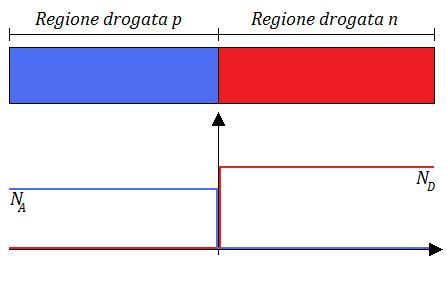
\includegraphics[scale=0.55]{7.png}
			\caption{Semiconduttore con drogaggi differenti all’equilibrio ($T = 0^\degree K$)}
			\label{fig:im-7}
		\end{figure}
	\end{center}
	In un materiale di tipo $n$ dorgato non uniformemente abbiamo:
	$$J_n = 0 \implies q\mu_n n E + q D_n \frac{dn}{dx} = 0$$
	ma sappiamo che è:
	$$E = -\frac{d\varphi}{dx}$$
	$$D_n = \frac{KT}{q}\mu_n$$
	e quindi, sostituendo, possiamo scrivere:
	$$0=-\cancel{q}\cancel{\mu_n} n \frac{d\varphi}{dx} + \cancel{q} \frac{KT}{q}\cancel{\mu_n} \frac{dn}{dx} \implies \frac{d\varphi}{dx} = \frac{KT}{q} \cdot \frac{1}{n} \cdot \frac{dn}{dx}$$
	$$\rightarrow \int_{\varphi(n_1)=\varphi}^{\varphi(n_1)=\varphi_2} \frac{d \varphi}{\cancel{dx}} = \int_{n(x_1)=n_1}^{n(x_2)=n_1} \frac{KT}{q} \frac{1}{n} \frac{dn}{\cancel{dx}} = \frac{KT}{q} \int_{n_1}^{n_2} \frac{1}{n} dn$$
	che, integrando, porta a:
	$$\varphi_2 - \varphi = \frac{KT}{q} \cdot \ln \frac{n_2}{n_1}$$
	Allora:
	\begin{itemize}
		\item Conoscendo la differenza di concentrazione in due punti, possiamo calcolare il potenziale
		\item Conoscendo la differenza di potenziale in due punti, possiamo calcolare la concentrazione
	\end{itemize}
	Da questa considerazione possiamo decidere arbitrariamente che esiste un punto $x_0$ in cui, all’equilibrio, sia:
	$$\begin{cases} \varphi = 0 \\ n = 0 \\ p = 0 \end{cases}$$
	Allora abbiamo:
	$$\varphi(x) = \frac{KT}{q} \cdot \ln \frac{n(x)}{n_0} \iff n(x) = n_0 \cdot e^{\frac{q\varphi(x)}{KT}}$$
	Lo stesso ragionamento si può applicare imponendo $J_p = 0$. \\
	In questo caso sarebbe:
	$$\varphi(x) = -\frac{KT}{q} \cdot \ln \frac{p(x)}{p_0} \iff p(x) = p_0 \cdot e^{-\frac{q\varphi(x)}{KT}}$$
	\subsection{Giunzione $pn$}
	\subsubsection{Intervallo $(-w_p; w_n)$}
	Sappiamo con ragionevolezza che nell’intervallo $(-w_p; w_n)$ il potenziale sarà:
	$$0 < \varphi < \psi_b$$
	Tuttavia sappiamo anche che, per $\varphi$ anche di poco maggiore di zero (risultato necessariamente verificato per $x > -w_p$), sarà:
	$$\varphi > 0$$
	$$p(x) = p_0 \cdot e^{-\frac{q\varphi(x)}{KT}}$$
	$$p(x) \gg p_0 \approx N_A$$
	Dalla parte opposta, avremo invece, necessariamente:
	$$\varphi < \psi$$
	$$n(x) = n_0 \cdot e^{-\frac{q\varphi(x)}{kT}}$$
	$$n(x) \ll n_0 \approx N_D$$
	Dunque in tutto l’intervallo $(-w_p; w_n)$ \textbf{la concentrazione di elettroni e lacune è trascurabile}. \\
	Questa regione è detta \textbf{regione svuotata}. \\
	Il termine “svuotata” non indica che non vi siano portatori di carica ma solo che essi sono in una concentrazione trascurabile rispetto alle concentrazioni delle regioni neutre.
	\section{Giunzione pn in equilibrio}
		\subsection{La Giunzone \textit{pn}}
	\label{sub:pn}
	Premessa: \textbf{La giunzione $pn$ è il primo dispositivo elettronico che verrà introdotto in questo corso, la sua struttura sarà alla base di gran parte dei dispositivi elettronici più complessi}.\\\\
	Mantenendoci nelle condizioni di equilibrio e di bidimensionalità, vogliamo drograre un blocco di semiconduttore con concentrazioni uniformi di atomi accettori e donatori.\\\\
	Il punto in cui si passa dalla regione drogata di tipo $p$ (cioè con atomi accettori) e la regione di tipo $n$ (con atomi donatori) è detto giunzione metallurgica o più semplicemente giunzione.\\\\
	In condizione di equilibrio sappiamo che è:
	$$J_n = J_p = 0$$
	Possiamo aspettarci che la maggior parte dei fenomeni di diffusione si concentri nei pressi del punto di giunzione.\\
	Conseguentemente possiamo anche ipotizzare che esista una coordinata $w_n$ ed una sua duale $-w_p$ oltre le quali non si notano gli effetti perturbativi dovuti alla giunzione. \\
	Allora il dispositivo è diviso in quattro regioni:
	\begin{enumerate}
		\item una regione drogata $p$ che non risente della giunzione
		\item una regione drogata ( $p$ ) che risente della giunzione
		\item una regione drogata ($n$) che risente della giunzione
		\item una regione drogata ($n$) che non risente della giunzione
	\end{enumerate}
	I casi 1 e 4 sono già stati studiati in precedenza.
	\begin{center}
		\begin{figure}[h]
			\centering
			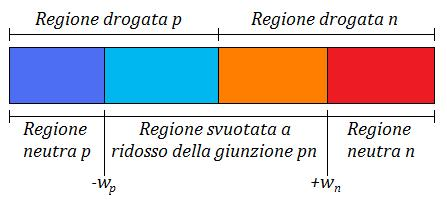
\includegraphics[scale=0.55]{8.png}
			\caption{Schema di una giunzione $pn$ e delle quattro zone in cui si può ipotizzare di suddividerla}
			\label{fig:im-8}
		\end{figure}
	\end{center}
	\subsubsection{Intervallo $(-\infty; -w_p)$}
	\label{subsub:int-pn1}
	Questa regione è detta zona neutra di tipo $p$.\\\\
	In questo intervallo abbiamo:
	$$p \approx \underbrace{N_A}_{\text{N di accettatori}}$$
	$$n \approx \frac{\overbrace{n_i^2}^{\text{Ricordando }p\cdot n = n_i^2}}{N_A}$$
	$$\rho = q(N_D - N_A + p - n) = 0$$
	Inoltre deve essere valida l’uguaglianza:
	$$J_p = q\mu_p p E - qD_p \frac{dp}{dx} = 0$$
	ma siccome il secondo membro è nullo (la derivata di una costante è sempre nulla) deve essere nullo anche il primo membro e dunque sarà: $E = 0$ $(\underbrace{E}_{=0} = \underbrace{- \frac{d \varphi}{dx}}_{=0})$.\\\\
	Il potenziale dovrà essere costante (se il campo elettrico, che è la derivata del potenziale, è nullo il potenziale dovrà essere necessariamente costante). \\
	Allora possiamo decidere che il potenziale $\varphi$ sia nullo.
	\subsubsection{Intervallo $(-w_p; w_n)$}
	\label{subsub:int-pn2}
	Sappiamo con ragionevolezza che nell’intervallo $(-w_p; w_n)$ il potenziale sarà:
	$$0 < \varphi < \psi_b$$
	Tuttavia sappiamo anche che, per $\varphi$ anche di poco maggiore di zero (risultato necessariamente verificato per $x > -w_p$), sarà:
	$$\varphi > 0$$
	$$p(x) = p_0 \cdot e^{-\frac{q\varphi(x)}{KT}}$$
	$$p(x) \gg p_0 \approx N_A$$
	Dalla parte opposta, avremo invece, necessariamente:
	$$\varphi < \psi$$
	$$n(x) = n_0 \cdot e^{-\frac{q\varphi(x)}{kT}}$$
	$$n(x) \ll n_0 \approx N_D$$
	Dunque in tutto l’intervallo $(-w_p; w_n)$ \textbf{la concentrazione di elettroni e lacune è trascurabile}. \\
	Questa regione è detta \textbf{regione svuotata}. \\
	Il termine “svuotata” non indica che non vi siano portatori di carica ma solo che essi sono in una concentrazione trascurabile rispetto alle concentrazioni delle regioni neutre.
	\subsubsection{Intervallo $(-w_p; 0)$}
	\label{subsub:int-pn3}
	In questo intervallo non abbiamo portatori mobili. ({\color{red}* DA RIVEDERE})\\\\
	Allora in questa regione la densità di carica è:
	$$\rho = q(-N_A + p - n) = -qN_A \qquad \{ p,n \to 0$$
	poiché $p$ ed $n$ sono trascurabili per piccole variazioni della concentrazione.\\\\
	Inoltre:
	$$\frac{dE}{dx} = \frac{\rho}{\varepsilon}$$
	Conseguentemente:
	$$\frac{dE}{dx} = \frac{-qN_A}{\varepsilon}$$
	da cui:
	$$dE = -\frac{qN_A}{\varepsilon}dx \overbrace{\implies}^{\int_{E(-w_p)}^{E(n)} dE = \int_{-w_p}^{n} - \frac{qE}{\varepsilon} dn} E(x) - \underbrace{E(-w_p)}_{=0} = -\frac{qN_A}{\varepsilon}(x + w_p)$$
	Per continuità con l’intervallo $(-\infty; -w_p)$, avremo $E(-w_p) = 0$.
	$$E(0) = -\frac{qN_A}{\varepsilon}(w_p)$$
	Allora nell’intervallo in questione il campo elettrico è una retta con coefficiente angolare negativo.\\\\
	Infine il potenziale è:
	$$E = - \frac{d \varphi}{dx} \rightarrow \frac{d\varphi}{dx} = \frac{qN_A}{\varepsilon}(x + w_p) \implies d\varphi = \frac{qN_A}{\varepsilon}(x + w_p)dx$$
	che, integrando da $-w_p$ ad $x$, porta a:
	$$\varphi(x) - \varphi(w_p) = \frac{qN_A}{\varepsilon} \cdot \frac{(x + w_p)^2}{2} = \frac{qN_A}{2\varepsilon}(x - w_p)^2$$
	Anche in questo caso, per continuità con l’intervallo $(-\infty; -w_p)$, avremo $\varphi(w_p) = 0$.
	$$\varphi(0) = \frac{qN_A}{2\varepsilon}(w_p)^2$$
	\subsubsection{Intervallo $(0; w_n)$}
	\label{subsub:int-pn4}
	Applicando ragionamenti similari a quelli visti nel,'intervallo \ref{subsub:int-pn3} otteniamo una densità di carica:
	$$\rho = qN_D$$
	La positività della costante è dovuta al fatto che, in questa regione, gli ioni fissi portano carica positiva.\\\\
	Per il campo elettrico avremo invece:
	$$E\left(x\right)\overbrace{=}^{\frac{dE}{dx}=\frac{qN_{0}}{E}\rightarrow\int_{E(w_n)}^{E(n)} dE=\int_{w_n}^{n}dx}\frac{qN_D}{\varepsilon}\left(x-w_n\right)$$
	che è una retta con coefficiente angolare positivo ed ordinata di origine negativa.
	$$E\left(0\right)=\frac{qN_D}{\varepsilon}\left(-w_n\right)$$
	Infine il potenziale si calcola in modo simile a quanto visto per l’intervallo $(-w_p; 0)$.
	$$\begin{cases} E=\frac{qN_d}{\varepsilon}\left(x-w_n\right) \\ E=-\frac{d\varphi}{dx}\end{cases}
	\;
	\Rightarrow-d\varphi=\frac{qN_d}{\varepsilon}\left(x-w_n\right)dx
	\rightarrow \int_{\varphi(w_{n})}^{\varphi(0)} -d\varphi \int_{w_{n}}^{0}\frac{q N_D}{\varepsilon}\left(x-w_{n}\right)dx$$
	Integrando da $\varphi\left(0\right)$ a $\varphi\left(w_n\right)=\psi_b$ otteniamo:
	$$\varphi\left(x\right)=\psi_b-\frac{qN_D}{2\varepsilon}\left(x-w_p\right)^2$$
	\subsubsection{Intervallo $(w_n; +\infty)$}
	\label{subsub:int-pn5}
	Questa regione è detta \textbf{zona neutra di tipo $n$}.\\\\
	In questa regione valgono tutti i ragionamenti visti nell'intervallo \ref{subsub:int-pn1} con l’unica differenza che non possiamo imporre arbitrariamente il valore di $\varphi$.\\\\
	In questo intervallo abbiamo:
	$$n\approx N_D$$
	$$p\approx\frac{n_i^2}{N_D}$$
	$$\rho=q\left(N_D-N_A+p-n\right)=0$$
	Inoltre deve essere valida l’uguaglianza:
	$$J_n=q\mu_{np}pE-qD_n\frac{dn}{dx}=0\implies E=0$$
	In questo caso non possiamo porre nuovamente il potenziale a zero poiché esso deve essere misurato in relazione al valore $\varphi=0$ imposto in precedenza. \\
	Dalla relazione ricavata nella sezione \ref{sub:app-mod} abbiamo:
	$$\varphi\left(x>w_n\right)=\frac{KT}{q}\cdot\ln\frac{N_D N_A}{n_i^2}$$
	e, siccome $\frac{KT}{q}$ \textbf{deve essere un potenziale} solitamente si indica con $V_T$ ed è detta \textbf{tensione termica}.\\
	A temperatura ambiente abbiamo:
	$$V_T=25 \ \mathrm{mV}$$
	Il valore del potenziale nella zona neutra $n$ è indicato con $\psi_b$ ed è detto \textbf{potenziale barriera} poiché deve fungere da barriera contro la diffusione dei portatori di carica.
	\subsubsection{Grafici}
	I grafici seguenti (grafici \ref{fig:image3} e grafici \ref{fig:image4}) mostrano le principali caratteristiche di una giunzione $p_n$ nelle quattro regioni.
	\begin{figure}[h]
		
		\begin{subfigure}{0.5\textwidth}
			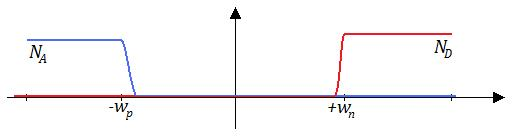
\includegraphics[width=0.9\linewidth]{9.png} 
			\caption{Concentrazione di atomi accettori e donatori in un diodo a giunzione $pn$ a temperatura ambiente}
			\label{fig:im-9}
		\end{subfigure}
		\begin{subfigure}{0.5\textwidth}
			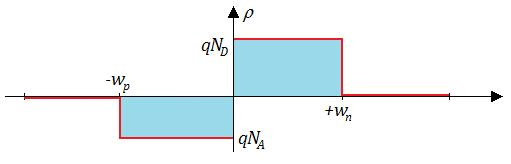
\includegraphics[width=0.9\linewidth]{10.png}
			\caption{Grafico della densità di carica in un diodo a giunzione $pn$}
			\label{fig:im-10}
		\end{subfigure}
		
		\caption{}
		\label{fig:image3}
	\end{figure}
	\begin{figure}[h]
		
		\begin{subfigure}{0.5\textwidth}
			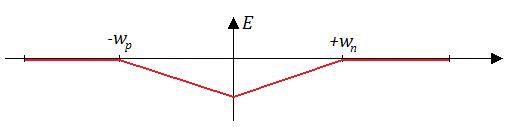
\includegraphics[width=0.9\linewidth]{11.png} 
			\caption{Campo elettrico in un diodo a giunzione $pn$}
			\label{fig:im-11}
		\end{subfigure}
		\begin{subfigure}{0.5\textwidth}
			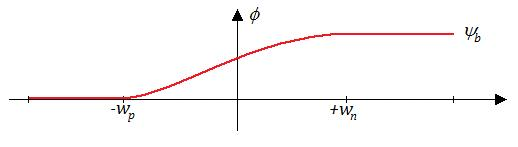
\includegraphics[width=0.9\linewidth]{12.png}
			\caption{Potenziale in un diodo a giunzione $pn$}
			\label{fig:im-12}
		\end{subfigure}
		
		\caption{}
		\label{fig:image4}
	\end{figure}
	Si noti che è:
	$$q N _ { A } w _ { p } = q N _ { D } w _ { n }$$
	Da questa relazione notiamo che la regione si svuota in maniera inversamente proporzionale alla concentrazione poiché le aree azzurre in figura \ref{fig:im-10} devono essere uguali.\\\\
	Oltre ad indicare che la giunzione si comporta quasi come un condensatore, questa relazione ci consente di ridurre di una ingognita le nostre equazioni.
	\subsection{Validazione}
	I risultati ed i grafici ottenuti nella sezione \ref{sub:pn}, si basano su una ipotesi: che $-w_p$ e $w_n$ siano entrambi compatibili con le dimensioni fisiche del dispositivo. \\
	Dobbiamo ora valutare se l’ipotesi è corretta o meno.\\\\
	Sappiamo che il campo elettrico si può calcolare in due modi differenti a seconda che consideriamo la zona svuotata $n$ o nella zona svuotata $p$. \\
	Siccome le due zone si congiungono in $x = 0$, in quel punto il campo dovrà, per continuità, essere lo stesso sia che venga calcolato da destra sia che venga calcolato da destra. \\
	Abbiamo ricavato in precedenza che deve essere:
	$$qN_A w_p = qN_D w_n$$
	Ragionando in modo analogo per il potenziale otteniamo che deve risultare:
	$$\varphi(x)=\psi_{b}-\frac{qN_{A}}{2\varepsilon}\left(x-w_{P}\right)^{2} \overbrace{\rightarrow}^{\text{Le zone si congiungono in }x=0} \frac{qN_A}{2\epsilon} w_p^2 = \psi_b - \frac{qN_D}{2\epsilon} w_n^2$$
	che è un’equazione in due incognite.\\\\
	Allora possiamo mettere le due equazioni a sistema e risolvere per sostituzione.
	$$\begin{cases} 
		qN_A w_p = qN_D w_n \\ 
		\frac{qN_A}{2\varepsilon} w_p^2 = \psi_b - \frac{qN_D}{2\varepsilon} w_n^2 
	\end{cases} 
	\implies 
	\begin{cases} 
		w_p = \frac{N_D}{N_A} w_n \\ 
		\psi_b = \frac{q}{2\varepsilon} \left( N_A w_p^2 + N_A w_n^2 \right) 
	\end{cases}$$
	$$\psi_b = \frac{q}{2\varepsilon} \left( N_A \left( \frac{N_D}{N_A} w_n \right)^2 + N_A w_n^2 \right) = \frac{qN_D^2 w_n^2}{2\varepsilon} \left( \frac{1}{N_A} + \frac{1}{N_D} \right)$$
	Sfruttando ora il fatto che
	$$\psi_b = \frac{KT}{q} \ln \frac{N_D N_A}{n_i^2}$$
	e sciogliendo il quadrato facendo la radice di ambo i membri, ricaviamo un valore numerico per $w_n$ e $w_p$:
	$$w_n = \frac{1}{N_D} \sqrt{\frac{2\varepsilon \psi_b}{q \left( \frac{1}{N_A} + \frac{1}{N_D} \right)}}$$
	$$w_p = \frac{1}{N_A} \sqrt{\frac{2\varepsilon \psi_b}{q \left( \frac{1}{N_A} + \frac{1}{N_D} \right)}}$$
	Tali valori, con parametri tipici, si attestano sulla dimensione di qualche micron. \\
	Allora \textbf{è sufficiente che il blocchetto di semiconduttore abbia dimensioni superiori a qualche micron} perché l’ipotesi sia soddisfatta ed il ragionamento sia valido.
	\subsection{Considerazioni}
	Possiamo inoltre calcolare l’ampiezza totale della regione svuotata.
	$$w \doteq w_p + w_n = \left( \frac{1}{N_A} + \frac{1}{N_D} \right) \sqrt{\frac{2\varepsilon\psi_b}{q \left( \frac{1}{N_A} + \frac{1}{N_D} \right)}} = \sqrt{\frac{2\varepsilon\psi_b}{q} \left( \frac{1}{N_A} + \frac{1}{N_D} \right)}$$
	Da questo risultato notiamo che la regione svuotata è tanto più piccola quanto più è drogato il materiale. \\
	Conseguentemente, se una parte del materiale è più drogata dell’altra, avremo una regione svuotata asimmettrica più piccola nella zona maggiormente drogata.\\\\
	Inoltre, dai grafici, notiamo che il campo elettrico ha verso opposto rispetto all’asse $x$. \\
	Dunque il campo ha un effetto di trascinamento delle lacune verso la zona $p$ e degli elettroni verso la zona $n$ che contrasta l’effetto diffusivo dovuto alla differenza di concentrazione. \\
	Abbiamo dunque una differenza di potenziale tra le due zone.\\\\
	Questa differenza di potenziale non produce tuttavia energia all’esterno (si avrebbe una violazione del principio di conservazione dell’energia): attaccando una lampadina ai capi delle regioni drogate questa non si accende. \\
	Questo risultato si spiega considerando che la giunzione tra il metallo ed il semiconduttore ha effetti simili alla giunzione $pn$ e deve essere nuovamente studiata in dettaglio. \\
	Anche fra la zona $p$ ed il metallo dunque si sviluppa una differenza di potenziale (detta \textbf{differenza di potenziale di contatto} ed indicata da $\psi_{cp}$ o $\psi_{cn}$) (Dove $C$ indica la zona conduttiva). \\
	Allora dovrà essere:
	$$\underbrace{\psi_b}_{\underset{\text{di Barriera}}{\text{Potenziale}}} + \underbrace{\psi_{cp}}_{\underset{\text{Contatto Zona $p$ e $c$}}{\text{Potenziale di}}} + \underbrace{\psi_{cn}}_{\underset{\text{Contatto Zona $c$ e $n$}}{\text{Potenziale di}}} = 0$$
	La differenza di potenziale di contatto è dipendente solamente dalla configurazione fisica del sistema e non dalla corrente che lo attraversa. \\
	Un contatto di questo tipi è detto \textbf{contatto ohmico}.
	\begin{center}
		\begin{figure}[h]
			\centering
			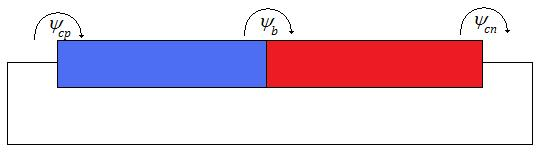
\includegraphics[scale=0.55]{13.png}
			\caption{Diodo a giunzione $pn$ collegato ad un filo di rame}
			\label{fig:im-13}
		\end{figure}
	\end{center}
%************************************************************************************************************************************************************************************
	\section{Diodo a giunzione pn: principio di funzionamento}
	\subsection{Funzionamento}
	\label{sub:funz-pn}
	Fino ad ora abbiamo studiato il comportamento del nostro oggetto in condizione di equilibrio. \\
	Vogliamo adesso studiarne il funzionamento fuori equilibrio: agganciamo un generatore di tesione $V$ al sistema (figura \ref{fig:im-14}).
	\begin{center}
		\begin{figure}[h]
			\centering
			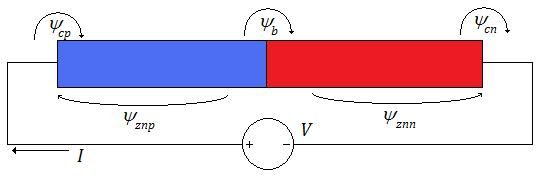
\includegraphics[scale=0.55]{14.png}
			\caption{Applicazione di un generatore di tensione al diodo}
			\label{fig:im-14}
		\end{figure}
	\end{center}
	All’equilibrio, cioè con $V = 0$, abbiamo, per la legge di Kirchoff:
	$$\psi_{cp} + \psi_{b_0} + \psi_{cn} = 0$$
	dove $\psi_{b_0}$ è il potenziale di barriera all’equilibrio.\\\\
	Usciamo dalla condizione di equilibrio: al variare di $V$ dovrà variare anche $\psi_b$. \\
	Tuttavia, lo abbiamo studiato in precedenza, le zone neutre si comportano come resistenze. \\
	Le cadute di potenziale sulle zone neutre sono indicate con $\psi_{znp}$ e $\psi_{znn}$. \\
	Allora, nuovamente per la legge di Kirchoff, abbiamo:
	$$V + \psi_{cp} - \psi_{znp} + \psi_b - \psi_{znn} - \psi_{cn} = 0$$
	Ipotizziamo che i contatti siano ohmici e supponiamo che i ragionamenti qualitativi fatti nella condizione di equilibrio siano ancora validi\footnote{Supponiamo cioè che di ragionare in condizione di piccolo scostamento dalla condizione di equilibrio.}. \\
	Sotto queste ipotesi, la corrente sarà qualitativamente piccola e, conseguentemente, le cadute di potenziale sulle zone neutre siano qualitativamente piccole. \\
	Quantifichiamo il termine \textbf{piccolo} come:
	$$\psi_{znp}, \psi_{znn} \ll \psi_b$$
	Allora possiamo semplificare l’equazione di maglia\footnote{Questa semplificazione non sarà più accettabile quando l’ipotesi di piccolo scostamento cadrà.} in:
	$$0 + \psi_{cp} - 0 + \psi_{b_0} - 0 - \psi_{cn} = 0$$
	Sottraendo membro a membro le due equazioni ottenute per la condizione fuori equilibrio abbiamo:
	$$V + \psi_b - \psi_{b_0} = 0$$
	da cui ricaviamo che il potenziale di barriera, in condizione di piccolo scostamento dall’equilibrio, è pari al potenziale di barriera in condizione di equilibrio diminuito della tensione applicata:
	$$\psi_b = \psi_{b_0} - V$$
	Dunque applicando una tensione positiva abbassiamo la barriera di potenziale mentre applicando una tensione negativa alziamo la barriera di potenziale.
	$$V > 0 \Longrightarrow \psi_b > \psi_{b_0}$$
	$$V < 0 \Longrightarrow \psi_b < \psi_{b_0}$$
	Sfruttando il grafico di figura \ref{fig:im-15} notiamo due comportamenti differenti in base alla tensione applicata.
	\begin{center}
		\begin{figure}[h]
			\centering
			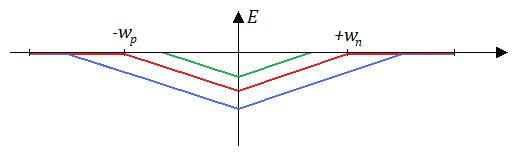
\includegraphics[scale=0.55]{15.png}
			\caption{Una differenza di potenziale modifica l’influenza del campo elettrico}
			\label{fig:im-15}
		\end{figure}
	\end{center}
	\quad\\
	Ricordiamo che $E= -grad(V)$.\\\\
	Se $V$ è positivo, abbiamo un abbassamento del campo ed il termine diffusivo è più importante del termine di trascinamento. \\
	Di conseguenza la corrente sarà positiva.\\\\
	Se invece $V$ è negativo abbiamo un innalzamento del campo ed il termine di trascinamento è più forte rispetto al termine di diffusione. \\
	Di conseguenza la corrente sarà negativa.
	\begin{table}[h][ht]
		\centering
		\begin{tabular}{|c|c|c|}
			\hline
			\textbf{Tensione} & \textbf{Effetti} & \textbf{Corrente} \\ \hline
			$V > 0$ & Trascinamento $<$ Diffusione & $I > 0$ \\ \hline
			$V = 0$ & Trascinamento = Diffusione & $I = 0$ \\ \hline
			$V < 0$ & Trascinamento $>$ Diffusione & $I < 0$ \\ \hline
		\end{tabular}
		\caption{Effetto vincente rispetto a differenti valori di tensione}
		\label{tab:table-2}
	\end{table}
	La differenza fondamentale è dovuta alla differenza della popolazione su cui agisce l’effetto:
	\begin{itemize}
		\item La corrente di diffusione agisce sui portatori maggioritari e quindi basta una ridotta variazione di tensione per avere una grande variazione di corrente
		\item La corrente di trascinamento agisce sui portatori minoritari e quindi una ridotta variazione di tensione porta ad una variazione di corrente molto ridotta.
	\end{itemize}
	Il comportamento è graficato in figura \ref{fig:im-16}.
	\begin{center}
		\begin{figure}[h]
			\centering
			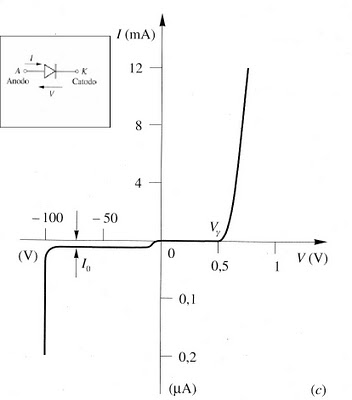
\includegraphics[scale=0.55]{16.png}
			\caption{Caratteristica e simbolo grafico di un diodo a giunzione $pn$}
			\label{fig:im-16}
		\end{figure}
	\end{center}
	Il dispositivo appena studiato è detto \textbf{diodo a giunzione $pn$} e viene rappresentato simbolicamente come una freccia che punta nella direzione in cui la corrente procede con facilità ed una barriera per il verso opposto.\\\\
	Il diodo a giunzione $pn$ ha due regioni di funzionamento: una detta \textbf{diretta} (ON) (quando $V$ ed $I$ sono positive) ed una detta \textbf{inversa} (OFF) (con $V$ ed $I$ negative).\\\\
	La caratteristica del diodo a giunzione $pn$ è modellabile come:
	$$I = I_S \left( e^{\frac{qV}{kT}} - 1 \right)$$
	In questo modello:
	\begin{itemize}
		\item Il valore ($-1$) è necessario per far passare dall’origine la curva esponenziale che altrimenti passerebbe nel punto ($I = 1$) per una tensione nulla
		\item La costante ($I_{S}$) (la corrente inversa di saturazione) è il valore di corrente cui tende asintoticamente il valore della corrente quando si applicano valori di corrente molto negativi
	\end{itemize}
	Sperimentalmente si nota che il modello così ricavato funziona bene solo quando tutte le ipotesi iniziali sono rispettate. \\
	Tuttavia se la tensione eccede un certo valore negativo, la corrente ricomincia a crescere a grande velocità risultando fortemente negativa.\\\\
	La tensione per cui avviene questo fenomeno è detta tensione di scarica o \textbf{tensione di break-down} ed è dovuta al fatto che, quando la tensione negativa eccede un certo valore, anche il campo elettrico inizia a generare coppie elettrone lacuna.\\\\
	L’ipotesi caduta è dunque la trascurabilità dell’azione del campo rispetto all’azione diffusiva.\\\\
	Aumentando troppo la tensione positiva e tracciando la curva su scala logaritmica, otteniamo il comportamento graficato in figura \ref{fig:im-17}.
	\begin{center}
		\begin{figure}[h]
			\centering
			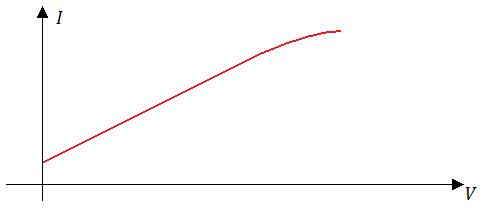
\includegraphics[scale=0.55]{17.png}
			\caption{Corrente in funzione della tensione in scala logaritmica}
			\label{fig:im-17}
		\end{figure}
	\end{center}
	L’ipotesi caduta in questo caso è la trascurabilità delle cadute sulle zone neutre poiché non è più vero che sia:
	$$\psi_{znp}, \psi_{znn} \ll \psi_b$$
	\begin{center}
		\begin{figure}[h]
			\centering
			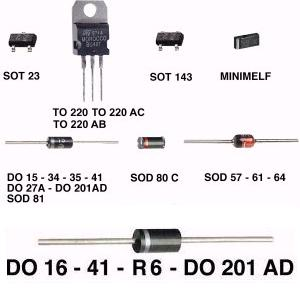
\includegraphics[scale=0.55]{18.png}
			\caption{Esempi di diodi in commercio}
			\label{fig:im-18}
		\end{figure}
	\end{center}
%************************************************************************************************************************************************************************************
	\section{Diodo a giunzione pn: applicazioni circuitali elementari}
	\subsection{Applicazione del Modello a Soglia}
	La "dimostrazione" del circuito raddrizzatore si trova negli appunti nella sezione "2.7 Utilità del diodo"
	\subsubsection{Circuito Raddrizzatore}
	Vediamo ora di applicare il modello a soglia al circuito raddrizzatore di Figura \ref{fig:im-25}.
	\begin{center}
		\begin{figure}[h]
			\centering
			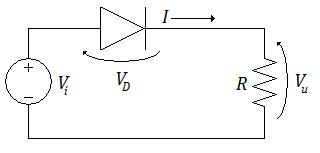
\includegraphics[scale=0.55]{25.png}
			\caption{Raddrizzatore a semionda}
			\label{fig:im-25}
		\end{figure}
	\end{center}
	Dall’equazione di maglia di Kirchhoff e dalla legge di Ohm abbiamo:
	$$V_i - V - V_u = 0$$
	$$V_u = RI$$
	Incontriamo ora il primo problema del nostro modello approssimato: avendo due regioni di funzionamento dobbiamo risolvere due volte il sistema e controllare che i risultati così ottenuti siano compatibili con le ipotesi di funzionamento formulate\footnote{In generale avendo $n$ diodi, si dovranno analizzare e verificare $2^n$ regioni di funzionamento. Il limite di questo approccio è duplice: bisogna identificare in quali ambiti esso è applicabile e, per grandi circuiti, il numero di calcoli cresce in modo esponenziale.}.\\\\
	Il modello a soglia impone che:
	$$\begin{cases} I = 0 & \text{per } V < V_\gamma \\ 
		V = V_\gamma & \text{per } I > 0 \end{cases}$$
	In questo caso è (Diodo OFF):
	$$\begin{cases} I = 0 \longrightarrow V_u = \underbrace{0}_{R \cdot 0} \\
		V < V_\gamma \ V - V_i - V_u = 0 \end{cases} \implies V_i < V_\gamma$$
	ed il modello risulta corretto.\\\\
	In questo caso è (Diodo ON):
	$$\begin{cases} I > 0 \longrightarrow V_u > 0 \\ 
		V < V_\gamma \longrightarrow \underbrace{V_u = V_i - V_\gamma}_{\textbf{Pendenza 1: Retta traslata}} \end{cases} \implies V_i > V_\gamma$$
	ed il modello risulta corretto.\\\\
	Vediamo il grafico in figura \ref{fig:im-26}
	\begin{center}
		\begin{figure}[h]
			\centering
			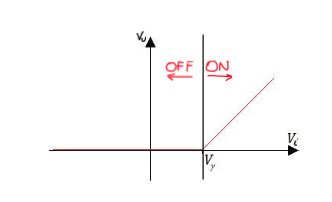
\includegraphics[scale=0.55]{26.png}
			\caption{Caratteristica $V \rightarrow I$ di un raddrizzatore}
			\label{fig:im-26}
		\end{figure}
	\end{center}
	\subsubsection{Circuito Limitatore Positivo}
	Prendiamo ora in considerazione il circuito in figura \ref{fig:im-27}
	\begin{center}
		\begin{figure}[h]
			\centering
			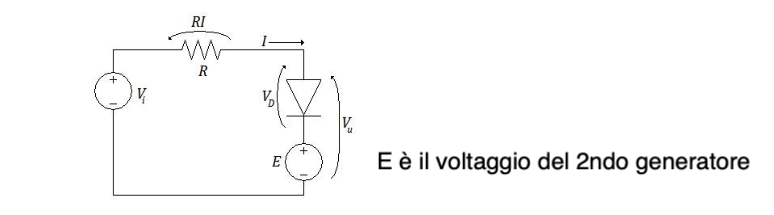
\includegraphics[scale=0.55]{27.png}
			\caption{Circuito limitatore positivo}
			\label{fig:im-27}
		\end{figure}
	\end{center}
	Ancora una volta abbiamo:
	$$V_i - RI - V_u = 0$$
	$$V_u = V_D + E$$
	In questo caso abbiamo (Diodo OFF):
	$$\begin{cases} I = 0 \\ 
		I = \frac{V_i - V_u}{R} \text{(Dall'eq. di Kirc qui sopra)}\end{cases} \implies \underbrace{V_i = V_u}_{\text{Bisettrice della prima parte}}$$
	$$\begin{cases} V_D < V_\gamma \\ 
		V_D = V_u - E \end{cases} \implies V_u - E < V_\gamma$$
	da cui ricaviamo:
	$$V_i - E < V_\gamma \implies V_i < E + V_\gamma$$
	Dunque il modello è corretto.\\\\
	In questo caso abbiamo (Diodo ON):
	$$\begin{cases} V_D = V_\gamma \longrightarrow V_u = V_\gamma + E \\ 
		I > 0 \longrightarrow V_i - V_u > 0 \longrightarrow V_i > V_u \end{cases} \implies V_i > E + V_\gamma$$
	Dunque il modello funziona.\\\\
	Vediamo il grafico in figura \ref{fig:im-28}
	\begin{center}
		\begin{figure}[h]
			\centering
			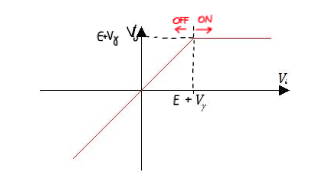
\includegraphics[scale=0.55]{28.png}
			\caption{Caratteristica $V \rightarrow I$ di un limitatore positivo}
			\label{fig:im-28}
		\end{figure}
	\end{center}
	Questo circuito può servire a limitare i picchi di tensione positiva.\\\\
	Si noti che variando il valore di $E$ è possibile aumentare o diminuire arbitrariamente il valore della limitazione.
	\subsubsection{Circuito Limitatore Negativo}
	Prendiamo ora in considerazione il circuito in figura \ref{fig:im-29} (Utilizziamo lo stesso metodo del precedente).
	\begin{center}
		\begin{figure}[h]
			\centering
			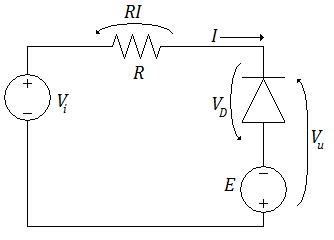
\includegraphics[scale=0.55]{29.png}
			\caption{Circuito limitatore negativo}
			\label{fig:im-29}
		\end{figure}
	\end{center}
	Allora per l’equazione di maglia di Kirchhoff è:
	$$V_i + RI = V_u$$
	$$V_u = -E - V_D$$
	In questo caso abbiamo (Diodo OFF):
	$$\begin{cases} I = 0 \longrightarrow V_u = V_i \\ 
		V_D < V_\gamma \\ 
		V_D = -E - V_i \end{cases} \implies -E - V_u < V_\gamma \implies V_u > -E - V_\gamma$$
	In questo caso abbiamo (Diodo ON):
	$$\begin{cases} V_D = V_\gamma \longrightarrow V_u = -(E + V_\gamma) \\ 
		I > 0 \longrightarrow I = \frac{-V_i + V_u}{R} \longrightarrow V_i < V_u \end{cases} \quad \implies V_i < -(E + V_\gamma)$$
	Dunque il modello funziona.
	Vediamo il grafico in figura \ref{fig:im-30}
	\begin{center}
		\begin{figure}[h]
			\centering
			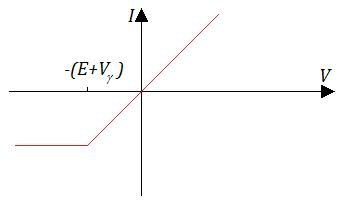
\includegraphics[scale=0.55]{30.png}
			\caption{Caratteristica $V \rightarrow I$ di un limitatore negativo}
			\label{fig:im-30}
		\end{figure}
	\end{center}
	\subsubsection{Limitatore Doppio}
	\subsubsection{Rivelatore di massimo}
	\subsubsection{Rivelatore di minimo}
%************************************************************************************************************************************************************************************
	\section{Raddrizzatore a doppia semionda}
	\subsection{Raddrizzatore a doppia semionda}
	Analizziamo il circuito in figura \ref{fig:im-35}
	\begin{center}
		\begin{figure}[h]
			\centering
			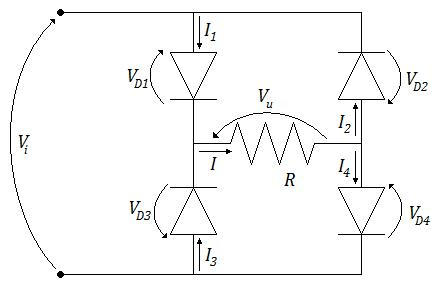
\includegraphics[scale=0.55]{35.png}
			\caption{Raddrizzatore a doppia semionda}
			\label{fig:im-35}
		\end{figure}
	\end{center}
	A prima vista, trattandosi di un circuito con quattro diodi, \textbf{dovremo analizzare sedici regioni di funzionamento differenti}. \\
	La Tabella \ref{tab:table-5} mostra le sedici possibili regioni. \\
	Sono indicate con una “X” le regioni fisicamente non ammesse.
	\begin{table}[ht]
		\centering
		\begin{tabular}{|c|c|c|c|c|c|c}
			\cline{3-7}
			\multicolumn{2}{c|}{} & OFF & OFF & ON & ON & \multicolumn{1}{c|}{\textbf{D3}} \\ \cline{3-7}
			\multicolumn{2}{c|}{} & OFF & ON & OFF & ON & \multicolumn{1}{c|}{\textbf{D4}} \\ \hline
			OFF & OFF & \ref{subsub:raddr-sopp-sem-off-off-off-off} & X & X & X & \multicolumn{1}{c}{} \\ \cline{1-6}
			OFF & ON  & X & X & \ref{subsub:raddr-sopp-sem-off-on-on-off} & X & \multicolumn{1}{c}{} \\ \cline{1-6}
			ON  & OFF & X & \ref{subsub:raddr-sopp-sem-on-off-off-on} & X & X & \multicolumn{1}{c}{} \\ \cline{1-6}
			ON  & ON  & X & X & X & X & \multicolumn{1}{c}{} \\ \cline{1-6}
			\textbf{D1} & \textbf{D2} & \multicolumn{5}{c}{} \\ \cline{1-2}
		\end{tabular}
		\caption{Tabella delle regioni di funzionamento del raddrizzatore a doppia semionda. \\ Le “X” indicano le zone fisicamente non possibili}
		\label{tab:table-5}
	\end{table}
	Analizzando preliminarmente il circuito possiamo ricavare che sia (Kirchoff alla maglia e al nodo):
	$$I = I_1 + I_3 = I_4 + I_2$$
	$$V_u = RI$$
	$$V_{D1} + V_{D2} + V_u = 0$$
	$$V_{D3} + V_{D4} + V_u = 0$$
	$$V_i - V_{D1} - V_u -V_{D3} = 0$$
	$$V_i + V_{D2} + V_u +V_{D4} = 0$$
	\subsubsection{D1 ON}
	Ipotizzando che il diodo $D1$ è acceso, otteniamo dalle equazioni di maglia che è:
	$$\begin{cases} I_1 > 0 \\ I_3 > 0 \\ I_4 \geq 0\end{cases} \implies I > 0 \implies V_u > 0$$
	$$V_{D1} - V_\gamma > 0$$
	$$V_{D2} = -(V_u + V_{D1})$$
	e di conseguenza avremo:
	$$V_{D2} < 0 < V_\gamma$$
	Ma allora quando il diodo $D1$ è acceso il diodo $D2$ sarà necessariamente spento.\\\\
	Sempre dalle equazioni di maglia notiamo quando $D1$ è acceso, sarà anche acceso il diodo $D4$. \\
	Infatti sarà:
	$$I_4 = I - I_2 \implies V_{D4} - V_\gamma > 0$$
	$$V_{D3} = -(V_u + V_{D4}) < 0$$
	Ed allora anche quando il diodo $D4$ risulta acceso il diodo $D3$ non può essere acceso.
	\subsubsection{D2 ON}
	Se il diodo $D2$ è acceso avremo:
	$$\begin{cases} I_2 > 0 \\ I_4 \geq 0 \end{cases} \implies I > 0 \implies V_u > 0$$
	$$V_{D2} = V_\gamma > 0$$
	$$V_{D1} = -(V_u + V_{D2}) < 0$$
	Ma allora se il diodo $D2$ è acceso, il diodo $D1$ deve essere spento e quindi:
	$$I_1 = 0$$
	Pertanto, siccome è:
	$$I = I_3 + I_1$$
	avremo che la corrente è fornita dal diodo $D3$ che dovrà dunque essere acceso.\\\\
	Ancora, sempre dalle equazioni di maglia, notiamo che il diodo non sono ragionevoli neppure le condizioni di accensione di un solo diodo.\\\\
	Ma allora \textbf{le regioni da analizzare si sono ridotte da sedici a tre}.
	\subsubsection{D1, D2, D3 e D4 OFF}
	\label{subsub:raddr-sopp-sem-off-off-off-off}
	In questa ipotesi la corrente è evidentemente nulla.
	$$I_1 = I_2 = I_3 = I_4 = 0 \implies I = 0$$
	Allora per la legge di Ohm, la tensione di uscita è nulla.
	$$V_u = 0$$
	Questa condizione è accettabile quando si ha:
	$$\begin{cases} V_{D1} < V_\gamma \\ V_{D2} < V_\gamma \\ V_{D3} < V_\gamma \\ V_{D4} < V_\gamma \end{cases}$$
	Usando le equazioni di maglia per i diodi $D1$ e $D4$ abbiamo:
	$$V_i - V_{D1} - V_u - V_{D4} = 0 \implies V_{D1} + V_{D4} = V_i$$
	da cui segue che deve essere:
	$$V_i < 2V_\gamma$$
	Procedendo nello stesso modo per $D2$ e $D3$, avremo:
	$$V_i + V_{D2} + V_{D3} + V_u = 0 \implies V_{D2} + V_{D3} = -V_i$$
	e quindi:
	$$V_i > -2V_\gamma$$
	Allora l’ambito di validità di questa regione è:
	$$-2V_\gamma < V_i < 2V_\gamma$$
	\subsubsection{D1 ON, D2 OFF, D3 OFF e D4 ON}
	\label{subsub:raddr-sopp-sem-on-off-off-on}
	Le ipotesi significano che la corrente è:
	$$I_1 = I_4 = I > 0$$
	Ma è anche:
	$$V_{D1} = V_{D4} = V_\gamma$$
	Sfruttiamo l’equazione di Kirchhoff vista nel sottosezione \ref{subsub:raddr-sopp-sem-off-off-off-off}:
	$$V_i - V_{D1} - V_u - V_{D4} \implies V_u = V_i - 2V_\gamma$$
	Questa condizione è verificata quando si ha:
	$$V_u > 0$$
	che, in relazione alla tensione di ingresso, è:
	$$V_i > 2V_\gamma$$
	\subsubsection{D1 OFF, D2 ON, D3 ON e D4 OFF}
	\label{subsub:raddr-sopp-sem-off-on-on-off}
	È la condizione duale a quelle della sottosezione \ref{subsub:raddr-sopp-sem-on-off-off-on} abbiamo:
	$$I_3 = I_2 = I > 0$$
	$$\begin{cases} V_{D2} = V_\gamma \\ V_{D3} = V_\gamma \end{cases}$$
	Sfruttiamo nuovamente l’equazione di maglia di Kirchhoff vista nella sottosezione \ref{subsub:raddr-sopp-sem-off-off-off-off}
	$$V_i + V_{D2} + V_{D3} + V_u \Longrightarrow V_u = -(V_i + V_{D2} + V_{D3}) \Longrightarrow V_u = -V_i - 2V_\gamma$$
	Queste ipotesi sono valide quando si ha:
	$$V_i < -2V_\gamma$$
	\subsubsection{Grafico e considerazioni}
	Il grafico della caratteristica è riportato in Figura \ref{fig:image5}
	\begin{figure}[h]
		
		\begin{subfigure}{0.5\textwidth}
			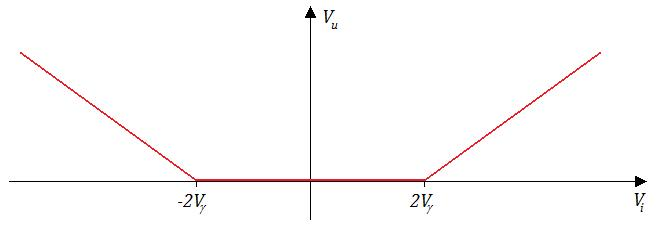
\includegraphics[width=0.9\linewidth]{36.png} 
			\caption{Caratteristica del raddrizzatore a doppia semionda}
			\label{fig:im-36}
		\end{subfigure}
		\begin{subfigure}{0.5\textwidth}
			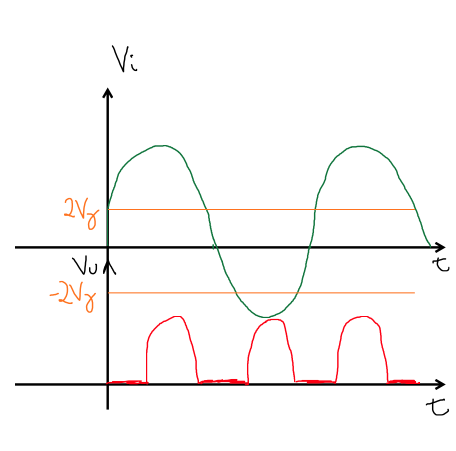
\includegraphics[width=0.9\linewidth]{37.png}
			\caption{}
			\label{fig:im-37}
		\end{subfigure}
		
		\caption{}
		\label{fig:image5}
	\end{figure}
	Questo circuito si comporta come un raddrizzatore a semionda per i valori positivi di $V_i$ che eccedono la soglia $2V_\gamma$. \\
	I valori di ingresso negativi che eccedono il valore $-2V_\gamma$ vengono riportati in positivo (vengono cioè “raddrizzati”).\\\\
	Per via di questo comportamento il circuito prende il nome di raddrizzatore a doppia semionda.\\\\
	Il raddrizzatore a doppia semionda è molto più efficiente di un raddrizzatore a semionda poiché, pur consentendo di ottenere un segnale a valor medio non nullo da un segnale a valor medio nullo, non elimina metà del segnale e, raddrizzandolo, porta ad un valor medio più elevato a parità di ingresso.\\\\
	La configurazione esaminata è detta ponte raddrizzatore di diodi ed è spesso disegnata come in Figura \ref{fig:im-38}
	\begin{center}
		\begin{figure}[h]
			\centering
			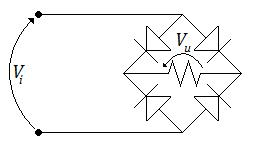
\includegraphics[scale=0.55]{38.png}
			\caption{Rappresentazione grafica classica del raddrizzatore a doppia semionda}
			\label{fig:im-38}
		\end{figure}
	\end{center}
%************************************************************************************************************************************************************************************
	\section{Raddrizzatore con filtro RC}
	\subsection{Convertitore alternata continua}
	\label{sub:ac-dc}
	I circuito raddrizzatori visti fino a questo momento, pur raddrizzando il segnale e portando un valor medio non nullo all’uscita, riportano comunque segnali periodici non costanti. \\
	Molti dispositivi domestici funzionano però a corrente continua. \\
	Dobbiamo trovare dunque un modo per estrarre la componente continua del segnale.\\\\
	Questo risultato si può ottenere facilmente aggiungendo un filtro passa basso che blocchi le componenti ad alta frequenza del segnale. \\
	Il più semplice filtro passa basso possibile è un condensatore che si comporta come un circuito aperto per frequenze nulle e come un corto circuito per frequenze elevate.\\\\
	Analizziamo ora cosa succede aggiungendo un filtro passa basso al raddrizzatore a singola semionda (per semplicità). \\
	Lo schema è riportato in Figura \ref{fig:im-39}
	\begin{center}
		\begin{figure}[h]
			\centering
			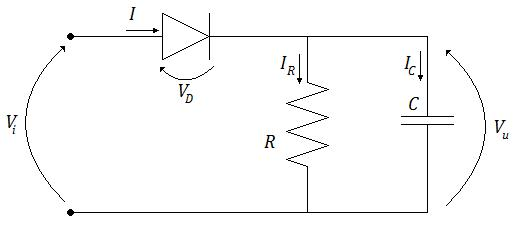
\includegraphics[scale=0.55]{39.png}
			\caption{L’aggiunta del condensatore di capacità $C$ consente di ridurre la variabilità del segnale di uscita}
			\label{fig:im-39}
		\end{figure}
	\end{center}
	L’aggiunta del condensatore di capacità $C$ modifica la caratteristica. \\
	Per le relazioni costitutive di resistenza e condensatore e per la legge di Kirchhoff abbiamo ora:
	$$I_R = \frac{V_u}{R}$$
	$$I_C = C \cdot \frac{dV_u}{dt}$$
	$$I = I_R + I_C \implies I = \frac{V_u}{R} + C \cdot \frac{dV_u}{dt}$$
	$$V_i - V_D - V_u = 0$$
	Ipotizziamo di avere in ingresso:
	$$V_i = V_m \sin(\omega t)$$
	con $V_m \gg V_\gamma$ (che è tipicamente verificata).
	\subsubsection{Diodo acceso}
	In questo caso è:
	$$V_D = V_\gamma \implies V_u = V_m \sin(\omega t)$$
	$$I > 0 \implies \frac{V_u}{R} + C \cdot \frac{dV_u}{dt} > 0$$
	Ma, per come è definito l’ingresso, il diodo sarà certamente attivo nell’intervallo $\left[0; \frac{T}{4}\right]$ dove $T$ è il periodo. \\
	Nell’intervallo $\left[\frac{T}{2}; \frac{3T}{4}\right]$ il diodo sarà invece necessariamente spento. \\
	Tuttavia nell’intervallo $\left(\frac{T}{4}; \frac{T}{2}\right)$ in cui si avrà $I = 0$ e cioè un punto, $t_{\text{OFF}}$ nel quale il diodo si spegne.
	\subsubsection{Spegnimento del diodo}
	Per calcolare $t_{\text{OFF}}$ imponiamo che sia:
	$$\frac{V_u}{R} + C \cdot \frac{dV_u}{dt} = 0$$
	$$-\frac{V_u}{R} = C \cdot \frac{dV_u}{dt}$$
	$$-\frac{V_m \sin(\omega t)}{R} = C \cdot \frac{d}{dt} [V_m \sin(\omega t)]$$
	$$-\frac{V_m}{R} \cdot \sin(\omega t) = V_m C \omega \cdot \cos(\omega t)$$
	$$\frac{\sin(\omega t)}{\cos(\omega t)} = -\omega RC$$
	$$\tan(\omega t_{\text{OFF}}) = -\omega RC \implies \omega t_{\text{OFF}} = -\arctan(\omega RC) \pm k\pi$$
	Allora abbiamo ricavato l’istante in cui il diodo si spegne. \\
	Ricordando che la tangente tende a $\pm\infty$ per $\alpha \rightarrow \pm\frac{\pi}{2}$ ed è periodica su un intervallo di durata $T = \pi$ è chiaro che il punto di spegnimento del diodo si troverà nell’angolo compreso tra $\frac{\pi}{2}$ e $\pi$.\\\\
	Riportato sul grafico di Figura \ref{fig:im-40} vediamo che il punto di spegnimento è tanto più vicino al tempo $\frac{T}{4}$ quanto più è elevato il valore di $RC$.
	Da $t_{\text{OFF}}$ in avanti il diodo risulta spento e la corrente sul diodo è nulla.
	\begin{center}
		\begin{figure}[h]
			\centering
			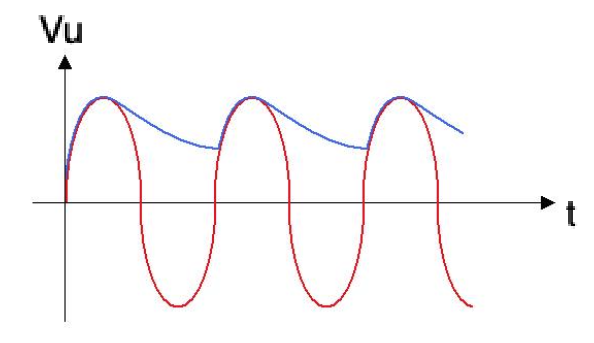
\includegraphics[scale=0.55]{40.png}
			\caption{Quando il diodo si spegne il condensatore inizia la sua fase di scarica}
			\label{fig:im-40}
		\end{figure}
	\end{center}
	$\omega_{t_{OFF}}$ è detto \textbf{Angolo di } {\color{red}* DA SISTEMARE!!!}
	\subsubsection{Diodo spento}
	Quando il diodo è spento abbiamo:
	$$I = 0$$
	$$\frac{V_u}{R} + C \cdot \frac{dV_u}{dt} = 0$$
	Ora però l’ingresso è nullo ed il circuito è semplificato come in Figura \ref{fig:im-41}
	\begin{center}
		\begin{figure}[h]
			\centering
			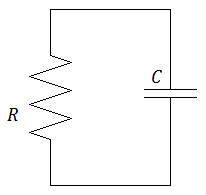
\includegraphics[scale=0.55]{41.png}
			\caption{Quando il diodo si spegne il circuito si semplifica ad un parallelo tra il condensatore e la resistenza}
			\label{fig:im-41}
		\end{figure}
	\end{center}
	Risolvendo l’equazione differenziale abbiamo:
	$$\frac{1}{RC} \int_{t_{\text{OFF}}}^t dt = \int_{V_u(t_{\text{OFF}})}^{V_u(t)} \frac{1}{V_u} dV_u$$
	$$\frac{t - t_{\text{OFF}}}{RC} = \ln \frac{V_u(t)}{V_u(t_{\text{OFF}})}$$
	$$V_u(t) = V_u(t_{\text{OFF}}) e^{\frac{t - t_{\text{OFF}}}{RC}}$$
	Allora l’uscita decresce con una curva esponenziale tanto più velocemente quanto più è piccolo il valore di $RC$.\\\\
	Questa condizione è verificata per tutti i valori per cui si ha:
	$$V_u > V_i$$
	Allora quando incontriamo nuovamente la sinusoide di ingresso torniamo ad utilizzare la relazione usata per il diodo acceso e quindi torniamo ad avere:
	$$V_u = V_i$$
%************************************************************************************************************************************************************************************
	\section{Effetti reattivi giunzione pn}
	\subsection{Problemi del diodo}
	Dalle simulazioni notiamo che, dimensionando opportunamente le costanti, possiamo utilizzare il convertitore esaminato nella sezione \ref{sub:ac-dc} per estrarre una funzione di uscita che si appoggi sul massimo del segnale di ingresso. \\
	Questa applicazione è molto utile quando si tratta di demodulare un segnale modulato in ampiezza.\\\\
	Fino a questo momento abbiamo applicato segnali tempo varianti all’ingresso di un circuito costituito da uno o più diodi. \\
	Aumentando la frequenza (senza aumentare le costanti $R$ e $C$) ci accorgiamo però di una anomalia non prevista dal modello.\\\\
	Il grafico di Figura \ref{fig:im-42} mostra come il diodo modifichi la sua caratteristica $V_i \to V_u$ all’aumentare della frequenza (il diodo fatica sempre più a spegnersi). \\
	Per una frequenza troppo elevata si arriva al limite per il quale il diodo non si spegne mai e continua a seguire sempre la curva di ingresso.
	\begin{center}
		\begin{figure}[h]
			\centering
			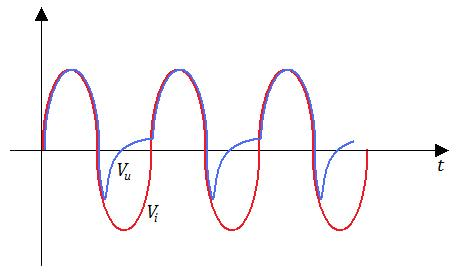
\includegraphics[scale=0.55]{42.png}
			\caption{Per frequenze elevate il diodo a giunzione $pn$ fatica sempre più a spegnersi \\ Per frequenze sufficientemente alte, il diodo resta sempre acceso}
			\label{fig:im-42}
		\end{figure}
	\end{center}
	Il modello visto fino ad ora ha funzionamento per due motivi:
	\begin{enumerate}
		\item Abbiamo usato il modello statico del diodo alla contare la variabile ( $t$ )
		\item Abbiamo sempre usato frequenze basse
	\end{enumerate}
	Tuttavia il diodo ha bisogno di un tempo non nullo per potersi spegnere. \\
	Allora per un periodo $T \to 0$, il diodo non avrà il tempo fisico di spegnersi.\\\\
	Nel grafico di Figura \ref{fig:im-43} l’area azzurra rappresenta la concentrazione di lacune che si spostano nel passaggio da polarizzazione diretta a polarizzazione inversa.
	\begin{center}
		\begin{figure}[h]
			\centering
			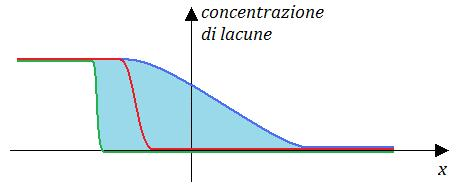
\includegraphics[scale=0.55]{43.png}
			\caption{Differenti concentrazioni di lacune per tensioni differenti: in rosso la situazione di equilibrio; in verde la condizione di polarizzazione inversa $V < 0$; in blu la condizione di polarizzazione diretta $V > 0$. \\ L’area azzurra è l’area necessaria allo spegnimento del diodo.}
			\label{fig:im-43}
		\end{figure}
	\end{center}
	Allora la carica non si può spostare in un tempo nullo (sarebbe necessaria un’energia infinita) e quindi abbiamo un tempo di reazione (effetti reattivi associati alla giunzione $p_n$) del diodo che sarà a sua volta non nullo.\\\\
	Il modello usato fino ad ora (\textbf{modello statico}) è utilizzabile solo per piccoli scostamenti dall’equilibrio e per segnali lentamente variabili nel tempo.
	\subsection{Modello Dinamico}
	Iniziamo ora lo studio di un modello migliore del diodo che tenga conto della variazione nel tempo. \\
	All’inizio dello studio del diodo a giunzione $p_n$ avevamo calcolato che la densità di carica nella regione svuotata fosse:
	$$Q_n = -Q_p = -\underbrace{qN_A}_{\rho} w_p$$
	dove:
	$$w_p = \frac{1}{N_A} \sqrt{\frac{2\varepsilon\psi_{B0}}{q\left(\frac{1}{N_A} + \frac{1}{N_D}\right)}} \implies Q_p = \sqrt{\frac{2\varepsilon q\psi_{B_0}}{\left(\frac{1}{N_A} + \frac{1}{N_D}\right)}}$$
	In ipotesi di piccolo scostamente avevamo inoltre visto che:
	$$\psi_B = \psi_{B_0} - V$$
	Allora possiamo ricavare la carica dinamica del diodo in funzione della tensione:
	$$Q(V) = \sqrt{\frac{2\varepsilon q(\psi_B - V)}{\left(\frac{1}{N_A} + \frac{1}{N_D}\right)}}$$
	che, nuovamente, è una funziune non lineare.\\\\
	Si noti che per $V = 0$ il valore della carica $Q_0 = Q(0)$ non passa per l’origine. \\
	La capacità del diodo è data dalla derivata della curva $Q(V)$
	$$DQ(V) = \frac{d}{dV}Q(V)$$
	e quindi, per comodità, useremo la curva $Q - Q_0$ in modo da ottenere $Q(0) = 0$ che non modifica la derivata.\\\\
	In questa condizione il diodo si comporta come un condensatore di capacità variabile (\textbf{diodo varicap}) ed era molto utilizzato nei primi televisori analogici a colori.
	Applicando una tensione $V > \psi_{B_0}$ abbiamo invece una soluzione assurda: la base della radice è negativa. \\
	In realtà, per $V = \psi_{B_0}$ abbiamo che il campo elettrico e la barriera di potenziale sono entrambi nulli. \\
	Ma se la barriera è nulla, la regione svuotata non esiste e di conseguenza non ha più senso parlare di piccolo scostamento.\\\\
	Allora la pendenza della curva della carica del diodo è detta capacità di svuotamento. \\
	In particolare la pendenza in $V = 0$ è detta capacità di giunzione all’equilibrio.\\\\
	Siccome la regione svuotata non esiste, dobbiamo considerare, per la carica, un secondo contributo dovuto alla carica dei portatori mobili. \\
	Si può dimostrare che il secondo contorbuto di carica dipende esponenzialmente dalla tensione applicata (cosa prevedibile in quanto la corrente cresce esponenzialmente in polarizzazione diretta). \\
	Questo secondo conturbuto è trascurabile per la polarizzazione inversa mentre è importante per la polarizzazione diretta.
	$$\begin{cases} J \propto \left(e^{\frac{V}{V_T}} - 1\right) \\ J \propto \frac{dn}{dx} \end{cases} \implies \frac{dn}{dx} \propto \left(e^{\frac{V}{V_T}} - 1\right) \implies n \propto \left(e^{\frac{V}{V_T}} - 1\right)$$
	Possiamo allora ottenere un modello un poco approssimato ma comunque sufficientemente preciso prendendo entrambe le componenti dominanti della carica nel diodo.
	$$\begin{cases} Q(V) = \sqrt{\psi_{B0} - V} & V < 0 \\ Q(V) = Q_S \left(e^{\frac{V}{V_T}} - 1\right) & V \geq 0 \end{cases}$$
	Tale modello è raffigurato in figura \ref{fig:im-44}.
	\begin{center}
		\begin{figure}[h]
			\centering
			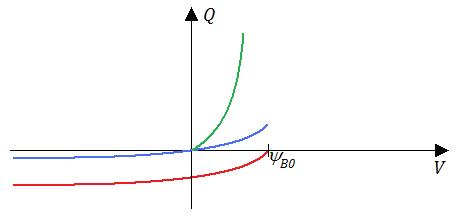
\includegraphics[scale=0.55]{44.png}
			\caption{Grafico del modello dinamico del diodo. In rosso la funzione $Q$ per $V < 0$; in blu la funzione $Q - Q_0$; in verde la funzione $Q$ per $V \geq 0$}
			\label{fig:im-44}
		\end{figure}
	\end{center}
	Riprendendo il modello statico possiamo sfruttare il fatto che sia:
	$$\begin{cases} I_0 = I_D \left(e^{\frac{V}{V_T}} - 1\right) \\ Q = Q_S \left(e^{\frac{V}{V_T}} - 1\right) \end{cases} \implies \frac{Q}{I_0} = \frac{Q_S \left(e^{\frac{V}{V_T}} - 1\right)}{I_D \left(e^{\frac{V}{V_T}} - 1\right)} = \frac{Q_S}{I_D} = \tau$$
	possiamo scrivere la carica in funzione della corrente od il contrario:
	$$Q = \tau I_D \iff I_D = \frac{Q}{\tau}$$
	Il valore $\tau$ è un tempo ed è il \textbf{tempo di vita medio dei portatori}. \\
	È cioè il tempo medio intercorso tra il momento in cui un portatore $p$ diffonde in zona $n$ ed il momento in cui esso si ricombina.\\\\
	Allora abbiamo ricavato un modello dinamico fortemente non lineare del diodo. \\
	Nuovamente introduciamo una semplificazione simile a quella vista per la corrente.
	$$\begin{cases}V<V_\gamma&\begin{cases}I_D=0\\Q\approx0\end{cases} \\ V=V_\gamma&\begin{cases}I_D>0\\Q>0\end{cases}\end{cases}$$
	Questo modello approssimato per la carica è meno preciso rispetto al modello statico visto per la carica. \\
	Il diodo dinamico è rappresentato come in Figura \ref{fig:im-45}.
	\begin{center}
		\begin{figure}[h]
			\centering
			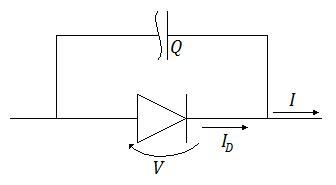
\includegraphics[scale=0.55]{45.png}
			\caption{Simbolo del modello dinamico del diodo}
			\label{fig:im-45}
		\end{figure}
	\end{center}
	La corrente al terminale di uscita del diodo è data da:
	$$I = I_{D} + \frac{dQ}{dt}$$
	Allora per frequenze basse possiamo riutilizzare le relazioni studiate per il caso statico (per tali frequenze $\frac{dQ}{dt}$ è infatti trascurabile). \\
	Questo diodo si può modellare sia con il controllo di corrente:
	$$I = I_{D} \left( e^{\frac{V}{V_{T}}} - 1 \right)$$
	sia con il modello a controllo di carica:
	$$I = \frac{Q}{\tau} = \frac{Qs \left( e^{\frac{V}{V_{T}}} - 1 \right)}{\tau}$$
	\subsection{Analisi Dinamica}
	\label{sub:analisi-din}
	Nella precedente sezione abbiamo introdotto il modello dinamico del diodo a giunzione $p_n$. \\
	Quanto esplicitato nella scorsa sezione è di estrema importanza poiché consente di determinare i limiti fisici dei circuiti digitali di nostro interesse. \\
	Il modello ricavato è descritto dalle equazioni:
	$$\begin{cases}V<V_\gamma&\begin{cases}I_D=0\\Q\approx0\end{cases} \\ V=V_\gamma&\begin{cases}I_D>0\\Q>0\end{cases}\end{cases}$$
	La carica è invece modellabile come:
	$$Q(V) = \sqrt{\frac{2\varepsilon q(\psi_B - V)}{\left(\frac{1}{N_A} + \frac{1}{N_D}\right)}} = \underbrace{\sqrt{\frac{2\varepsilon q\psi_B}{\left(\frac{1}{N_A} + \frac{1}{N_D}\right)}}}_{\text{carica all’equilibrio}} \cdot \sqrt{1 - \frac{V}{\psi{B0}}}$$
	Abbiamo infine completato il modello a soglia aggiungendo un condensatore in parallelo al diodo in modo da poter vedere, grazie a Kirchhoff, la corrente come somma delle due componenti statiche e dinamiche:
	$$I = I_{Statica} + I_{Dinamica}$$
	In questa sezione vedremo l’utilizzo del modello dinamico e l’analisi di un semplice circuito.\\\\
	Consideriamo il circuito di Figura \ref{fig:im-46} e supponiamo che la tensione di ingresso $V_i(t)$ sia maggiore di $V_\gamma$ per $t < 0$ e minore di zero per $t \geq 0$ (figura \ref{fig:im-48}).
	\begin{figure}[h]
		
		\begin{subfigure}{0.5\textwidth}
			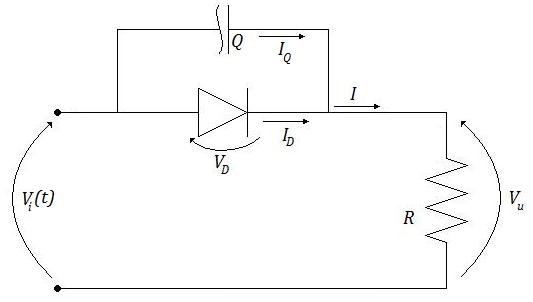
\includegraphics[width=0.9\linewidth]{46.png} 
			\caption{Circuito per l’analisi del comportamento dinamico del diodo}
			\label{fig:im-46}
		\end{subfigure}
		\begin{subfigure}{0.5\textwidth}
			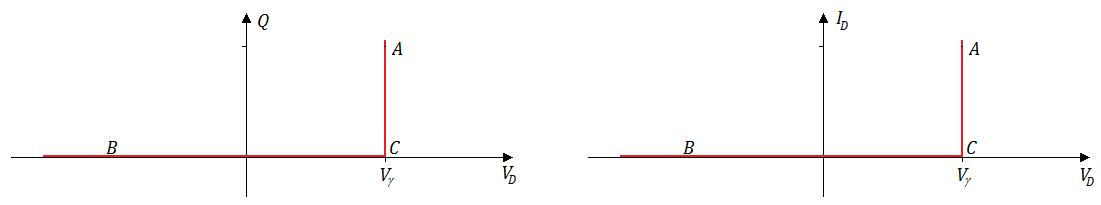
\includegraphics[width=0.9\linewidth]{47.png}
			\caption{Modello a soglia della concentrazione di carica $Q$ e della corrente $I_D$ del diodo}
			\label{fig:im-47}
		\end{subfigure}
		
		\caption{}
		\label{fig:image6}
	\end{figure}
	\subsubsection{Situazone per $t<0$}
	Il circuito in questione è già stato analizzato nel caso statico. \\
	Dallo schema circuitale, sfruttando le leggi di Ohm e Kirchhoff, abbiamo:
	$$V_u = RI$$
	$$V_i = V_D + V_u$$
	$$I = I_D + I_C \implies \begin{cases} I_D = \frac{Q}{\tau} \\ I_C = \frac{dQ}{dt} \end{cases} \implies I = \frac{Q}{\tau} + \frac{dQ}{dt}$$
	Per tempi negativi ($t < 0$) siamo in condizioni stazionarie e allora gli effetti reattivi non contano. \\
	Dunque l’analisi è già stata effettuata e allora l’uscita è costante:
	$$V_u = V_F - V_\gamma$$
	e siccome è $V_u = RI$, ricaviamo:
	$$I = \frac{V_F - V_\gamma}{R} \implies Q = \frac{\tau}{R} (V_F - V_\gamma)$$
	Allora la novità consiste nel fatto che la carica è diversa da zero (questo non è in contrasto con quanto detto: essere in condizioni statiche significa che i valori sono costanti e non necessariamente nulli).
	\subsubsection{Situazione per $t = 0^+$: transitorio $A \rightarrow C$}
	Per $t = 0$ abbiamo un transitorio: la commutazione dell’ingresso non si riflette istantaneamente sull’uscita. \\
	Aspettando un tempo sufficientemente elevato torneremo comunque ad una condizione statica nella quale avremo:
	$$\begin{cases} I = I_D = 0 \\ V_u = RI = 0 \end{cases} \implies V_D = V_i = -V_R$$
	Allora, nel transitorio, la corrente e la carica dovranno spostarsi da un valore positivo ad un valore negativo.\\\\
	Analizziamo il transitorio. \\
	Consideriamo l’istante $t = 0^+$. \\
	Siccome la carica non può variare istantaneamente sarà:
	$$Q(0^-) = \frac{V_F - V_\gamma}{R} \tau = Q(0^+)$$
	da cui ricaviamo che la tensione non può variare istantaneamente e quindi:
	$$V_D = V_\gamma$$
	Allora risulta:
	$$V_i = -V_R \implies V_u = V_i - V_D \implies -V_R - V_\gamma = -(V_R + V_\gamma)$$
	che è un valore negativo. \\
	Dunque la tensione di ustica presenta un gradino che porta da un valore positivo ad un valore negativo. \\
	Il fatto che questo punto sia esterno alla caratteristica statica dipende dal fatto che nel ricavarla non si era tenuto conto degli effetti dinamici del diodo.\\\\
	La corrente è data ora da:
	$$I = \frac{Q}{\tau} + \frac{dQ}{dt}$$
	e non è più possibile eliminare la derivata. \\
	Allora, riprendendo quanto detto prima e ricordando che nel tratto da $A$ a $C$ di Figura \ref{fig:im-47} la tensione è $V_D = V_\gamma$, risulta:
	$$\frac{Q}{\tau} + \frac{dQ}{dt} = \frac{-(V_R + V_\gamma)}{R} \implies \frac{dQ}{dt} = -\frac{1}{\tau} \left( Q + \frac{\tau}{R} (V_R + V_\gamma) \right)$$
	da cui si ricava:
	$$\frac{dQ}{Q + \frac{\tau}{R} (V_R + V_\gamma)} = -\frac{1}{\tau}$$
	che, integrata, porta a:
	$$\int_0^t -\frac{1}{\tau} dt = \int_{Q(0)}^{Q(t)} \frac{1}{Q + \frac{\tau}{R} (V_R + V_\gamma)} dQ$$ $$-\frac{t}{\tau} = \ln \left[ \frac{Q(t) + \frac{\tau}{R} (V_R + V_\gamma)}{Q(0) + \frac{\tau}{R} (V_R + V_\gamma)} \right] \implies e^{-\frac{t}{\tau}} = \frac{Q(t) + \frac{\tau}{R} (V_R + V_\gamma)}{Q(0) + \frac{\tau}{R} (V_R + V_\gamma)}$$
	Semplificando quanto appena ottenuto ricaviamo:
	$$Q(t) = \frac{\tau}{R} (V_F - V_\gamma) e^{-\frac{t}{\tau}} - \frac{\tau}{R} (V_R + V_\gamma)$$
	Allora nel transitorio la carica decade con una legge esponenziale ed una costante di tempo $\tau$. \\
	Analiticamente la carica tende asintoticamente al valore $-\frac{\tau}{R} (V_R + V_\gamma)$. \\
	Tuttavia, siccome abbiamo usato il modello a soglia, l’ambito di validità è ridotto ai valori tali per cui: $Q \geq 0$.\\\\
	Allora, la tensione di uscita resta costante e negativa fino al punto $C$ che è il punto tale per cui risulta $Q(C) = 0$. \\
	Parimenti la corrente sarà negativa e costante fino al punto $C$.\\\\
	Il tempo impiegato per raggiungere il valore zero dalla curva $Q(t)$ è il tempo di spegnimento del diodo.
	$$\left\{t_{\text{OFF}} = t \mid Q(t) = 0\right\} \implies \frac{\tau}{R} (V_F - V_\gamma) e^{-\frac{t}{\tau}} - \frac{\tau}{R} (V_R + V_\gamma) = 0$$ $$e^{-\frac{t}{\tau}} = \frac{V_R + V_\gamma}{V_F + V_\gamma} \implies t_{\text{OFF}} = \tau \cdot \ln \frac{V_F + V_F}{V_R + V_\gamma}$$
	Il tempo di spegnimento sarà sempre certamente maggiore di zero e non dipende dalla resistenza $R$ del circuito. \\
	Poiché questo tempo dipende solo dalle cariche interne al diodo, è detto \textbf{tempo di storage}.\\\\
	Il \textbf{tempo di spegnimento} è un valore molto importante poiché in base ad esso possiamo decidere se utilizzare o meno un dato diodo in un circuito.\\
	Un diodo sarà utilizzabile solo se il tempo di spegnimento è molto inferiore al tempo di commutazione.
	\subsubsection{Situazione per $t > 0$: transitorio $C \rightarrow B$}
	In questa situazione abbiamo cambiato la zona di funzionamento e, dal modello a soglia, è:
	$$\begin{cases} Q = 0 \\ I_D = 0 \end{cases}$$
	Allora la carica deve passare da zero a zero e non si spostano portatori. \\
	Dunque il transitorio è istantaneo. \\
	Inoltre, siccome in questo caso si ha $I = I_D$, la tensione di uscita è a sua volta nulla. \\
	Ai capi del diodo avremo ora una tensione pari a $-V_R$.
	\subsubsection{Grafici}
	La Figura \ref{fig:im-48} mostra i grafici di quanto ottenuto fino ad ora.
	\begin{center}
		\begin{figure}[h]
			\centering
			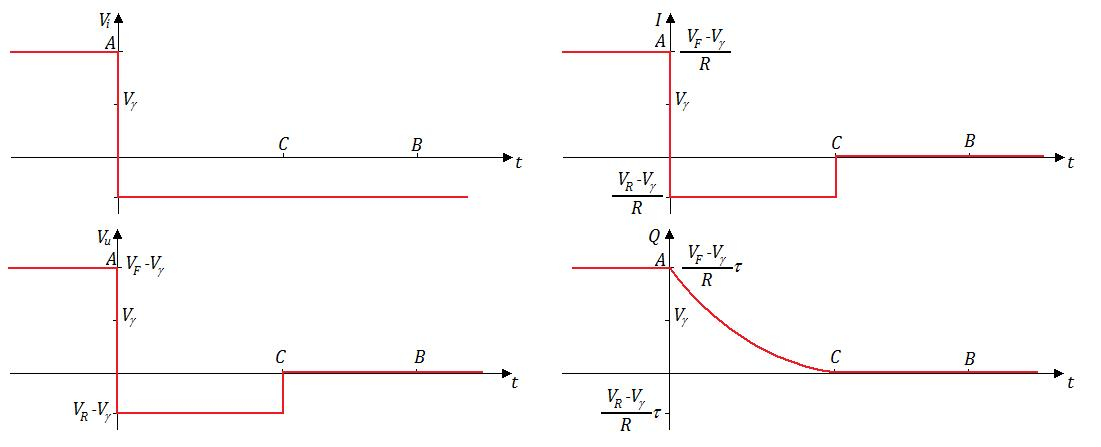
\includegraphics[scale=0.55]{48.png}
			\caption{Comportamento dinamico delle principali caratteristiche del diodo}
			\label{fig:im-48}
		\end{figure}
	\end{center}
	Dalle simulazioni e dai risultati sperimentali notiamo che, all’aumentare del valore di $R$ notiamo che il modello risulta sempre meno preciso. \\
	Questo è dovuto al fatto che abbiamo approssimato una curva esponenziale con una retta orizzontale imponendo:
	$$Q \approx 0$$
	Una migliore approssimazione è costituita dall’utilizzo di una retta obliqua (Figura \ref{fig:im-49}).
	\begin{center}
		\begin{figure}[h]
			\centering
			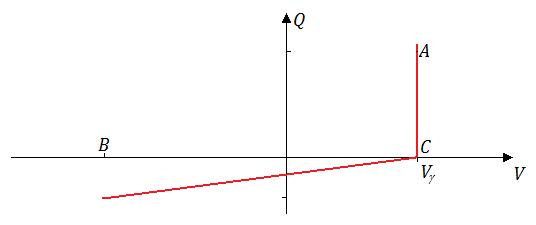
\includegraphics[scale=0.55]{49.png}
			\caption{Grafico che mostra una migliore approssimazione del comportamento dinamico del diodo. \\ Questo grafico spiega anche il differente comportamento per valori diversi di $R$.}
			\label{fig:im-49}
		\end{figure}
	\end{center}
	Sfruttando ora un condensatore normale di capacità $C$ abbiamo:
	$$I = C \cdot \frac{dV_u}{dt}$$
	$$V_u = RI \implies I = \frac{V_u}{R}$$
	$$\frac{V_u}{R} = -C \cdot \frac{d}{dt} (V_R + V_u)$$
	Ancora, dai grafici e dalle prove sperimentali, notiamo che mentre il diodo ha necessità di un certo lasso di tempo per lo spegnimento, l’accensione richiede un tempo pressoché nullo. \\
	Allora la non linearità del diodo statico si ritrova sul diodo dinamico.
%************************************************************************************************************************************************************************************
	\section{Transitori di commutazione raddrizzatore}
	Il transitorio di commutazione viene sviluppato qui: \ref{sub:analisi-din}
%************************************************************************************************************************************************************************************
	\section{Transistore bipolare a giunzione: principi di funzionamento}
	\subsubsection{Introduzione}
	Premessa: Si ricordi che il \textbf{diodo è un componente non lineare}.\\\\
	Nella scorsa sezione abbiamo analizzato il modello dinamico del diodo ed abbiamo notato che il suo comportamento varia fortemente dalla fase di spegnimento (che necessità di un tempo $t_{\text{OFF}}$ detto tempo di storage non nullo) alla fase di accensione (che richiede invece un tempo nullo).\\\\
	Abbiamo inoltre notato che, nonostante il tempo di storage sia indipendente dalla resistenza di carico, il recupero della condizione asintotica dipende proprio dalla resistenza di carico.\\\\
	Infine abbiamo mostrato che se il tempo di storage è paragonabile al periodo del segnale di ingresso, il diodo non riesce a spegnersi e quindi è come se il diodo stesso non fosse presente (il condensatore in parallelo al diodo lo cortocircuita). \\
	Allora esistono un periodo minimo ed una frequenza massima oltre i quali il modello non è più utilizzabile.
	\subsection{Diodo $npn$}
	Fino ad ora abbiamo ragionato utilizzando il diodo a giunzione $pn$ in cui la corrente circola prevalentemente in una sola direzione. Con il diodo abbiamo costruito sia gli AND sia gli OR. Resta però da realizzare il NOT che è piuttosto complesso da realizzare con i diodi.
	Ricordiamo che tutti i ragionamenti fatti sino ad ora per il diodo sono validi con alcune limitazioni:
	\begin{itemize}
		\item Lo scostamento alla regione di equilibrio deve essere ridotto
		\item Il diodo deve essere sufficientemente grande da poter essere partizionato in due regioni neutre ai margini ed in due regioni svuotate limitrofe alla giunzione
	\end{itemize}
	Costruiamo ora una struttura più complessa: la giunzione $npn$ che aggangia una regione $n$ ad ogni lato della regione $p$ (Figura 12.1).
	\begin{center}
		\begin{figure}[h]
			\centering
			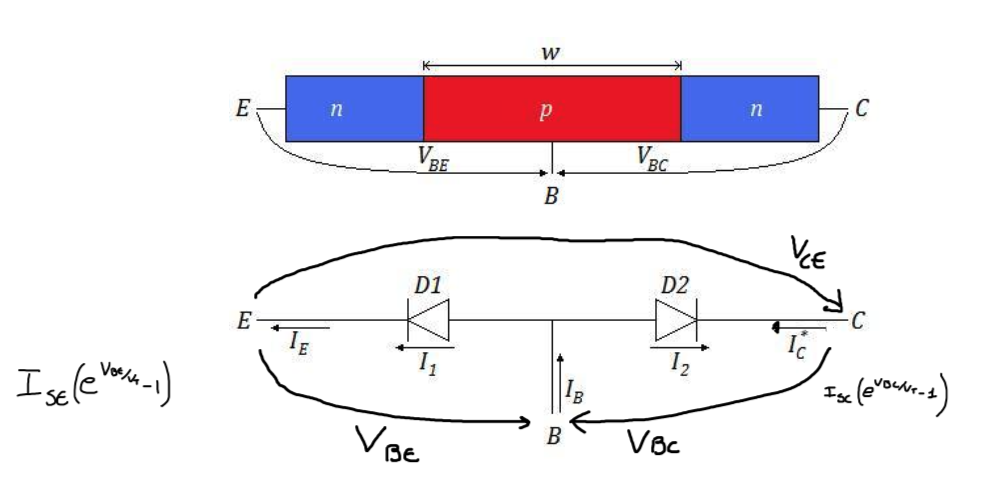
\includegraphics[scale=0.35]{50.png}
			\caption{Dispositivo composto da due diodi}
			\label{fig:im-50}
		\end{figure}
	\end{center}
	I terminali sono indicati come emettitore ($E$), base ($B$) e collettore ($C$).\\\\
	Possiamo pensare di analizzare il sistema appena costruito con quanto già sappiamo del diodo a giunzione $p_n$ poiché si tratta, in effetti, di un circuito composto da due diodi.\\\\
	Detta $w$ la \textbf{distanza tra le due regioni} $n$, abbiamo però due comportamenti differenti per la situazione in cui il diodo $D2$ è spento:
	\begin{enumerate}
		\item Per $w$ superiore a qualche micron, la corrente di collettore $I_C^*$ è trascurabile (allora il circuito si riduce al solo diodo $D1$ che abbiamo già studiato in precedenza):
		$$\begin{cases} V_{BE} > 0 \\ V_{BC} < 0 \end{cases} \implies \begin{cases} I_1 > 0 \\ I_2 = 0 \end{cases} \implies \begin{cases} I_B = I_E = I_1 \\ I_C^* = 0 \end{cases}$$
		Ricordando per i calcoli:
		$$V_{BE} - V_{BC} - V_{CE} = 0$$
		$$I_B + I_C = I_E \quad \text{Kirchoff}$$
		$\begin{cases}
			BE = \text{ON} \\
			BC = \text{OFF}
		\end{cases}$
		\item Per $w$ inferiore a qualche micron, la corrente di collettore $I_C^*$ è paragonabile alla corrente di emettitore $-I_E$ e la corrente di base $I_B$ è molto inferiore alle altre due correnti:
		$$\begin{cases} V_{BE} > 0 \\ V_{BC} < 0 \end{cases} \implies \begin{cases} I_1 > 0 \\ I_2 = 0 \end{cases} \implies \begin{cases} I_C^* = -I_E \\ I_B \ll I_C^* \end{cases}$$
	\end{enumerate}
	Le Figure \ref{fig:im-51} mostrano i diversi comportamenti del dispositivo in funzione della dimensione di $w$.
	\begin{center}
		\begin{figure}[h]
			\centering
			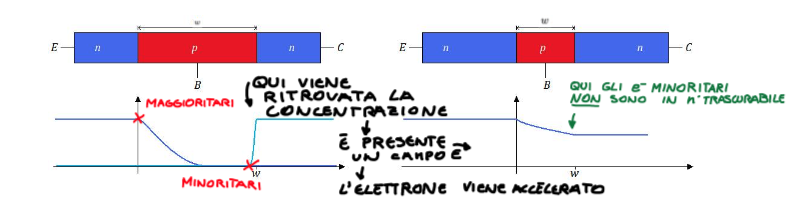
\includegraphics[scale=0.55]{51.png}
			\caption{Diversi comportamenti nella regione svuotata. \\ Una base di dimensioni sufficientemente elevate (a sinistra) consente di studiare il dispositivo come fatto in precedenza.}
			\label{fig:im-51}
		\end{figure}
	\end{center}
	Il modello precedente nel secondo caso non funziona poiché, se $w$ è troppo piccolo, la regione $p$ non è più partizionale in regioni svuotate e regioni neutre. \\
	Quando $w$ è di dimensioni inferiori a pochi micron, le due regioni $n$ hanno un effetto complementare sulla regione svuotata: gli elettroni hanno probabilità sempre maggiori di sopravvivere al passaggio nella base.\\\\
	In questo caso, la giunzione polarizzata in inversa trasporta molta carica grazie al supporto della giunzione polarizzata in diretta che pone nella base portatori minoritari recuperati poi dal collettore.\\\\
	Questo effetto è detto effetto transistor ed è alla base dei componenti detti transistori. \\
	In particolare il componente appena realizzato è detto transistore bipolare a giunzione (o BJT, bipolar junction transistor) ed è indicato con il simbolo di Figura \ref{fig:im-52}.
	\begin{center}
		\begin{figure}[h]
			\centering
			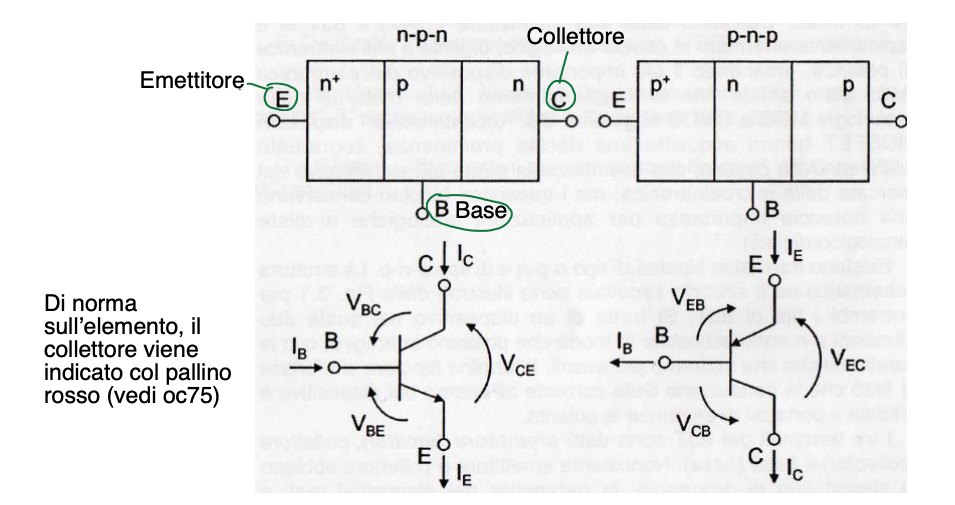
\includegraphics[scale=0.35]{52.png}
			\caption{Simboli grafici per la rappresentazione di un transistore npn (a sinistra) o pnp (a destra) in un circuito elettrico}
			\label{fig:im-52}
		\end{figure}
	\end{center}
%************************************************************************************************************************************************************************************
	\section{Modello di Ebers e Moll e caratteristiche parametriche BJT}
	\subsection{Modello di Ebers \& Moll}
	L’emettitore è così detto perché immette portatori nella base ove si trovano le lacune. \\
	Una parte sperabilmente piccola degli elettroni immessi nella base, ricombinerà con le lacune lì presenti. \\
	Tuttavia il collettore, recupererà una gran parte degli elettroni immessi nella base dall’emettitore.
	I flussi di lacune ed elettroni sono mostrati in Figura \ref{fig:im-53}.
	\begin{center}
		\begin{figure}[h]
			\centering
			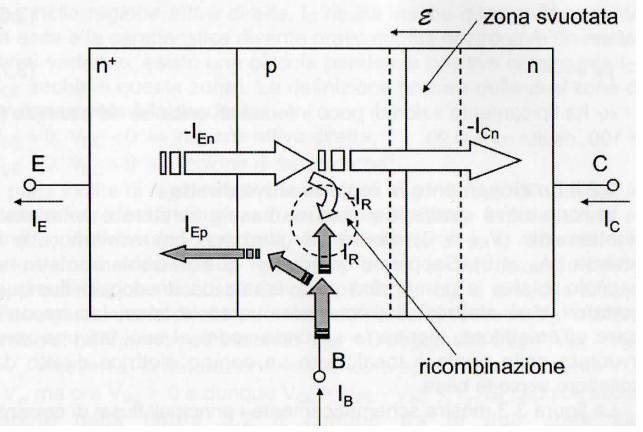
\includegraphics[scale=0.35]{53.png}
			\caption{Flussi di elettroni e lacune all’interno del modello di Ebers \& Moll}
			\label{fig:im-53}
		\end{figure}
	\end{center}
	Detta $I_t$ la corrente dovuta all’effetto transistor, possiamo utilizzare il modello studiato per il diodo e completarlo con l’aggiunta del termine $I_t$, definito, dalle legge di Kirchhoff, come (Che dall'equazione qui sotto notiamo avere 2 componenti):
	$$I_t = \underbrace{I_S \left( e^{\frac{V_{BE}}{V_T}} - 1 \right)}_{\text{Componente 1}} - \underbrace{I_S \left( e^{\frac{V_{BC}}{V_T}} - 1 \right)}_{\text{Componente 2}}$$
	Parimenti, possiamo definire le correnti sui due diodi, come:
	$$I_1 = I_{BES} \left( e^{\frac{V_{BE}}{V_T}} - 1 \right) \qquad \left(I_{BES} = I_{SE} - I_S\right)$$
	$$I_2 = I_{BCS} \left( e^{\frac{V_{BC}}{V_T}} - 1 \right) \qquad \left(I_{BCS} = I_{SC} + I_B\right)$$
	Notiamo che, siccome la corrente di collettore è elevata quando si è in regione di polarizzazione diretta, assumeremo che sia $I_C = -I_C^*$.\\\\
	I grafici dei due possibili BJT ($npn$ e $pnp$), sono riportati in Figura \ref{fig:im-52}. \\
	Utilizzeremo prevalentemente il modello $npn$.\\\\
	Il modello riportato in Figura \ref{fig:im-54} è chiamato Modello di Ebers \& Moll e funziona sufficientemente bene per le nostre applicazioni.
	\begin{center}
		\begin{figure}[h]
			\centering
			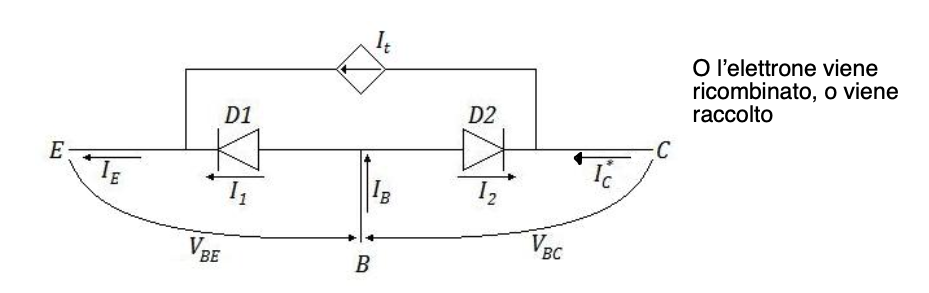
\includegraphics[scale=0.35]{54.png}
			\caption{Grafico del modello di Ebers \& Moll}
			\label{fig:im-54}
		\end{figure}
	\end{center}
	Il modello è descritto da:
	$$\begin{cases} 
		I_B = I_{BES} \left( e^{\frac{V_{BE}}{V_T}} - 1 \right) + I_{BCS} \left( e^{\frac{V_{BC}}{V_T}} - 1 \right) \\ 
		I_C = I_S \left( e^{\frac{V_{BE}}{V_T}} - 1 \right) - (I_{BCS} + I_S) \left( e^{\frac{V_{BC}}{V_T}} - 1 \right) \\ 
		I_E = (I_{BES} + I_S) \left( e^{\frac{V_{BE}}{V_T}} - 1 \right) - I_S \left( e^{\frac{V_{BC}}{V_T}} - 1 \right) 
	\end{cases}$$
	Si dice che il modello di \textbf{Ebers \& Moll} è in regione normale (o attiva diretta) quando si ha:
	$$\begin{cases} V_{BE} > 0 \\ V_{BC} < 0 \end{cases} \implies \begin{cases} V_B > V_E \\ V_B < V_C \end{cases} \implies V_E < V_B < V_C$$
	Allora possiamo controllare la corrente tra collettore ed emettitore agendo sulla tensione della base. \\
	Se $V_B$ è bassa, la corrente tra collettore ed emettitore è bassa; se $V_B$ è alta, la corrente tra collettore ed emettitore è alta.\\\\
	Per approfondire guardare appunti sezione "3.3 Semplificazioni"
	\subsection{Connessione in emettitore comune}
	Riprendiamo il circuito di Figura \ref{fig:im-67}
	\begin{center}
		\begin{figure}[h]
			\centering
			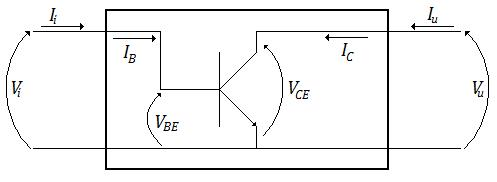
\includegraphics[scale=0.35]{67.png}
			\caption{Connessione in emettitore comune}
			\label{fig:im-67}
		\end{figure}
	\end{center}
	Dal modello di Ebers \& Moll definito in precedenza
	$$\begin{cases}
		I_B = I_{BES} \left( e^{\frac{V_{BE}}{V_T}} - 1 \right) + I_{BCS} \left( e^{\frac{V_{BC}}{V_T}} - 1 \right) \\
		I_C = I_S \left( e^{\frac{V_{BE}}{V_T}} - 1 \right) - (I_{BCS} + I_S) \left( e^{\frac{V_{BC}}{V_T}} - 1 \right) \\
		I_E = (I_{BES} + I_S) \left( e^{\frac{V_{BE}}{V_T}} - 1 \right) - I_S \left( e^{\frac{V_{BC}}{V_T}} - 1 \right)
	\end{cases}$$
	cerchiamo di esplicitare le correnti del tripolo in esame.
	$$\begin{cases} I_B(V_{BE}, V_{CE}) \\ I_C(V_{BE}, V_{CE}) \end{cases}$$
	La $V_{BC}$ non è definita nel modello.\\
	Fortunatamente, siccome la $V_{BC}$ non è indipendente dalle altre tensioni, possiamo scriverla come:
	$$V _ {B C} = V _ {B E} - V _ {C E} \Longrightarrow V _ {C E} = V _ {B E} - V _ {B C}$$
	\subsubsection{Ingresso}
	Allora possiamo vedere la corrente di ingresso come:
	$$I_B(V_{BE}, V_{CE}) = I_{BES} \left( e^{\frac{V_{BE}}{V_T}} - 1 \right) + I_{BCS} \left( e^{\frac{V_{BE} - V_{CE}}{V_T}} - 1 \right)$$
	Questa configurazione è però molto complessa poiché implica che la corrente $I_B$ dipende da una coppia di grandezze e quindi dovrebbe essere in un grafico tridimensionale. \\
	Dobbiamo allora ricavare un sistema più pratico.\\\\
	Una soluzione molto più pratica consiste nel tracciare una serie di curve bidimensionali parametriche fissando la $V_{CE}$ o la $V_{BE}$ in modo da ottenere una serie di funzioni di una sola variabile.
	$$I_B(V_{BE}, V_{CE}) \longrightarrow I_B(V_{BE}) \text{ con } V_{CE} = \text{costante}$$
	In condizione di funzionamento normale, ricaviamo che è:
	$$e^{\frac{V_{BE}}{V_T}} \gg e^{\frac{V_{BC}}{V_T}}$$
	$$I_B = I_{BES} \left( e^{\frac{V_{BE}}{V_T}} - 1 \right)$$
	ed allora l’intera famiglia di curve collassa sulla sola curva di Figura \ref{fig:im-68}.
	\begin{center}
		\begin{figure}[h]
			\centering
			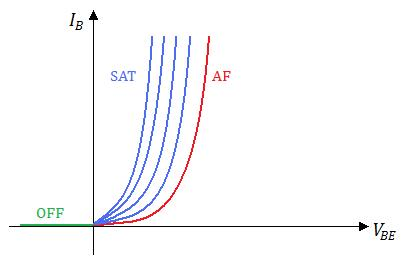
\includegraphics[scale=0.35]{68.png}
			\caption{Caratteristica dell’ingresso di un BJT}
			\label{fig:im-68}
		\end{figure}
	\end{center}
	Se invece ci poniamo nella regione di saturazione abbiamo:
	$$I_B(V_{BE}, V_{CE}) = I_{BES} \left( e^{\frac{V_{BE}}{V_T}} \right) + I_{BCS} \left( \frac{e^{\frac{V_{BE}}{V_T}}}{e^{\frac{V_{CE}}{V_T}}} \right)$$
	$$I_B = e^{\frac{V_{BE}}{V_T}} \left( I_{BES} + \frac{I_{BCS}}{e^{\frac{V_{CE}}{V_T}}} \right)$$
	e quindi la famiglia di curve presenta andamenti esponenziali moltiplicati per una costante tanto più grande quanto più $V_{CE}$ è piccolo.
	\subsubsection{Uscita}
	\label{subsub:conn-em-com-out}
	Vediamo ora cosa succede per la corrente di uscita.\\\\
	Analogamente a quanto visto prima è:
	$$I_C(V_{BE}, V_{CE}) \longrightarrow I_C(V_{CE}) \text{ con } V_{BE} = \text{costante}$$
	$$I _ { C } = I _ { S } \left( e ^ { \frac { V _ { B E } } { V _ { T } } } - 1 \right) - \left( I _ { B C S } + I _ { S } \right) \left( e ^ { \frac { V _ { B E } - V _ { C E } } { V _ { T } } } - 1 \right)$$
	In regione di funzionamento normale, il termine dovuto alla $V_{CE}$ è trascurabile e la curva di uscita risulta essere costante per valori costanti di $V_{BE}$:
	$$I _ { C } = I _ { S } \left( e ^ { \frac { V _ { B E } } { V _ { T } } } - 1 \right) = \beta _ { F } I _ { B }$$
	Questa condizione ha senso solo quando si ha:
	$$V _ { B E } > V _ { C E } \Longrightarrow I _ { S } \left( e ^ { \frac { V _ { C E } } { V _ { T } } } - 1 \right) > I _ { C }$$
	In saturazione abbiamo invece la condizione opposta a quella per il funzionamento in regione normale. \\
	La corrente di uscita è allora:
	$$I _ { C } = I _ { S } \left( e ^ { \frac { V _ { B E } } { V _ { T } } } \right) - \left( I _ { B C S } + I _ { S } \right) \left( \frac { e ^ { \frac { V _ { B E } } { V _ { T } } } } { e ^ { \frac { V _ { C E } } { V _ { T } } } } \right) < \beta _ { F } I _ { B }$$
	dove abbiamo trascurato le unità.\\\\
	La Figura \ref{fig:im-69} mostra l’uscita del BJT.
	\begin{center}
		\begin{figure}[h]
			\centering
			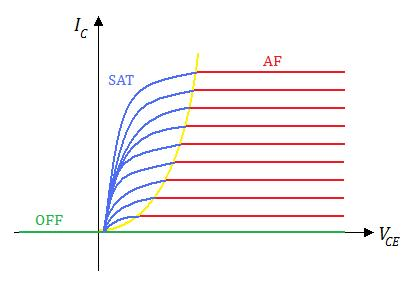
\includegraphics[scale=0.35]{69.png}
			\caption{Caratteristica dell’uscita di un BJT}
			\label{fig:im-69}
		\end{figure}
	\end{center}
	Dall’immagine si nota subito che tutte le curve della regione di saturazione passano per uno stesso punto che non è l’origine. \\
	In particolare l’uscita si annulla quando risulta essere:
	$$I _ { S } \left( e ^ { \frac { V _ { B E } } { V _ { T } } } \right) - \left( I _ { B C S } + I _ { S } \right) \left( \frac { e ^ { \frac { V _ { B E } } { V _ { T } } } } { e ^ { \frac { V _ { C E } } { V _ { T } } } } \right) = 0 \Longrightarrow e ^ { \frac { V _ { B E } } { V _ { T } } } = \frac { I _ { S } + I _ { B C S } } { I _ { S } } = \frac { 1 } { \alpha _ { R } }$$
	che è una costante. \\
	Passando ora ai logaritmi risulta:
	$$V _ { C E } = V _ { T } \cdot \ln \left( \frac { 1 } { \alpha _ { R } } \right)$$
	Il punto di attraversamento dell’asse delle ascisse dunque non dipende dalla tensione $V_{BE}$.\\\\
	Fisicamente la spiegazione di questo comportamento sta nel fatto che, all’aumentare della $V_{CE}$ il flusso che dal collettore porta elettroni in base diventa sempre più importante e, per valori sufficientemente elevati di $V_{CE}$ può anche dominare sul flusso che dall’emettitore porta gli elettroni al collettore.\\\\
	La Tabella \ref{tab:table-6} riassume quanto visto fino ad ora:
	\begin{table}[ht]
		\centering
		\begin{tabular}{|c|c|c|}
			\hline
			\textbf{Porta} & \textbf{Regione} & \textbf{Caratteristica} \\
			\hline
			\textbf{Ingresso} & Diretta & Famiglia collassata su una sola curva. \\
			\hline
			& Saturazione & Curve esponenziali crescenti al decrescere di $V_{CE}$. \\
			\hline
			& Interdizione & Corrente nulla. \\
			\hline
			\textbf{Uscita} & Diretta & Valori costanti per valori costanti di $V_{BE}$. \\
			\hline
			& Saturazione & Curve esponenziali decrescenti al decrescere di $V_{CE}$. \\
			\hline
			& Interdizione & Corrente nulla. \\
			\hline
		\end{tabular}
		\caption{Caratteristiche delle varie regioni di funzionamento del BJT}
		\label{tab:table-6}
	\end{table}
	\subsection{Relazione tra ingresso e uscita}
	\subsubsection{Riassunto}
	Il grafico di Figura \ref{fig:im-73} mostra quanto ottenuto dallo studio appena effettuato.
	\begin{center}
		\begin{figure}[h]
			\centering
			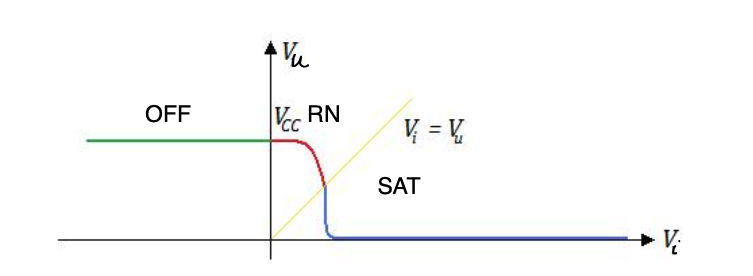
\includegraphics[scale=0.45]{73.png}
			\caption{Caratteristica di ingresso-uscita di un BJT ad emettitore comune. \\ In verde la caratteristica in interdizione, in rosso la caratteristica in regione normale ed in azzurro la caratteristica in saturazione.}
			\label{fig:im-73}
		\end{figure}
	\end{center}
	Questo circuito dispone di tre regioni con comportamenti qualitativamente molto differenti: due tratti a valori approssimativamente costanti (regione di interdizione e regione di saturazione) ed un tratto di raccordo (regione normale) che può avere una pendenza anche molto elevata.\\\\
	La pendenza è data dalla derivata dell’uscita. \\
	Siccome la parte con pendenza non nulla è dovuta alla regione normale, riprendiamo l’uscita in tale regione:
	$$V_u = V_{CC} - RI_S I_S \left( e^{\frac{V_i}{V_T}} - 1 \right)$$
	e ne calcoliamo la derivata nel punto $V_i = V_{i_0}$. \\
	Risulta:
	$$DV_u = -\frac{RI_S \cdot e^{\frac{V_{i_0}}{V_T}}}{V_T} = -\frac{RI_{C_0}}{V_T}$$
	Poiché siamo in regione normale, la $V_{i_0}$ è positiva ed allora possiamo trascurare il termine unitario. \\
	Allora la corrente di collettore è:
	$$I_C = I_S \cdot e^{\frac{V_{i_0}}{V_T}}$$
	Notiamo allora che la derivata ha un valore a denominatore molto basso ed un valore a numeratore molto più elevato. \\
	Allora la pendenza è molto elevata.\\\\
	Un circuito di questo tipo si presta bene alla realizzazione di una \textbf{porta NOT}. \\
	Consideriamo ad esempio i segnali:
	$$\begin{cases} V_L = 0 \\ V_H \approx V_{CC} \end{cases}$$
	La Tabella \ref{tab:table-7} mostra quanto appena detto:
	\begin{table}[ht]
		\centering
		\begin{tabular}{|c|c|}
			\hline
			$V_i$ & $V_u$ \\
			\hline 
			\hline
			$V_L$ & $V_H$ \\
			\hline
			$V_H$ & $V_L$ \\
			\hline
		\end{tabular}
		\caption{Funzionamento dell’invertitore logico realizzato con un BJT}
		\label{tab:table-7}
	\end{table}
	Si faccia attenzione al fatto che, pur non usando la regione normale di funzionamento del BJT, il componente si comporta come un invertitore proprio per la presenza della regione normale ad elevata pendenza.\\\\
	Per lavorare in regione normale è necessario progettare opportunamente il segnale di ingresso. \\
	Infatti se a $V_i = V_{i_0}$ corrisponde $V_u = V_{u_0}$ dovrà anche essere:
	$$V_i = V_{i_0} + \Delta V_i \longleftrightarrow V_u = V_{u_0} + \Delta V_u$$
	Per $\Delta V_i \rightarrow 0$ avremo allora:
	$$\frac{\Delta V_u}{\Delta V_i} = \frac{dV_u}{dV_i} = A_V \implies dV_u = A_V dV_i$$
	dove $A_V$ detto \textbf{guadagno di tensione}. \\
	Il guadagno di tensione può assumere valori anche molto elevati. \\
	Allora, quando si presenta un segnale variabile in un intervallo ristretto di $V_i$, il segnale di uscita varia in modo analogo all’ingresso amplificato di una costante $-A_V$. \\
	Allora il dispositivo studiato si comporta come un amplificatore analogico invertente.\\\\
	Il rispetto delle condizioni di piccolo spostamento e di alta pendenza è estremamente importante. \\
	Usare segnali con uno spostamento elevato provoca una distorsione del segnale di uscita rispetto al segnale di ingresso. \\
	La scelta della pendenza inficia invece il guadagno: più elevata è la pendenza, maggiore è l’amplificazione in ampiezza.\\\\
	Un’altra caratteristica del dispositivo studiato è che, mentre il segnale di ingresso è un segnale debole in potenza ed in corrente, il segnale di uscita è un segnale più forte sia in ampiezza sia in potenza. \\
	Questo fatto è dovuto al generatore di tensione $V_{CC}$.\\\\
	Ancora, pur avendo una $I_B$ libera di crescere indefinitamente, notiamo che la $I_C$ non può avere lo stesso comportamento. \\
	Quando si entra in regione di saturazione, la $I_C$ ha raggiunto il suo valore massimo (si dice quindi che è satura). \\
	Il problema è però dato dalla corrente $I_B$. \\
	La sua crescita esponenziale porta invece ad avere correnti di ingresso totalmente irragionevoli. \\
	Una possibile soluzione consiste nell’introdurre una resistenza sulla base (Figura \ref{fig:im-74}).
	\begin{center}
		\begin{figure}[h]
			\centering
			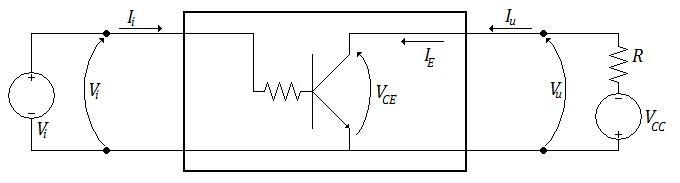
\includegraphics[scale=0.45]{74.png}
			\caption{L’inserimento della resistenza in base consente di limitare la corrente di ingresso a valori ragionevoli}
			\label{fig:im-74}
		\end{figure}
	\end{center}
%************************************************************************************************************************************************************************************
	\section{Invertitore RTL: caratteristica statica}
	\subsection{Invertitore RTL}
	\label{sub:inv-rtl}
	Consideriamo ora il circuito di Figura \ref{fig:im-77} e cerchiamo la caratteristica ingresso-uscita sfruttando il modello a soglia.
	\begin{center}
		\begin{figure}[h]
			\centering
			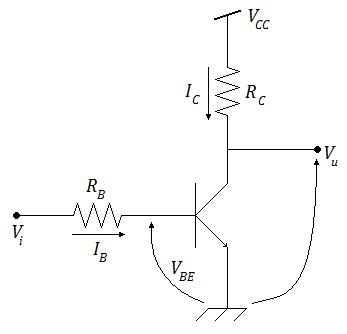
\includegraphics[scale=0.45]{77.png}
			\caption{Un invertitore RTL.}
			\label{fig:im-77}
		\end{figure}
	\end{center}
	\subsubsection{Considerazioni iniziali}
	Indipendentemente dalla regione di funzionamento possiamo dire:
	$$\begin{cases} I_B = \frac{V_i - V_{BE}}{R_B} \\ I_C = \frac{V_{CC} - V_u}{R_C} \\ V_{CE} = V_u \end{cases}$$
	\subsubsection{Regione di Interdizione}
	Dal modello a soglia sappiamo che è:
	$$\begin{cases} I_B = 0 \\ I_C = 0 \end{cases} \implies \begin{cases} V_i = V_{BE} \\ V_u = V_{CC} \end{cases}$$
	ma siccome è $V_i = V_{BE}$ e $V_u = V_{CE}$ risulta anche:
	$$\begin{cases} V_i < V_\gamma \\ V_{CC} = V_{CE} > V_{CESat} \end{cases}$$
	\subsubsection{Regione Normale}
	In regione normale è:
	$$\begin{cases} I_C = \beta_F I_B \\ I_B = \frac{V_i - V_\gamma}{R_B} \\ V_u = V_{CC} - R_C I_C \end{cases} \implies \begin{cases} V_u = V_{CC} - \frac{\beta_F R_C}{R_B} (V_i - V_\gamma) \\ V_i > V_\gamma \\ V_{CE} = V_u > V_{CESat} \end{cases}$$
	Notiamo che l’uscita è proporzionale all’ingresso secondo la funzione:
	$$V_u = V_{CC} - \frac{\beta_F R_C}{R_B} (V_i - V_\gamma)$$
	la cui derivata è:
	$$A_V = -\frac{\beta_F R_C}{R_B}$$
	che porta ad un guadagno lineare dato dal rapporto tra la resistenza di base e la resistenza di collettore.\\\\
	Per ricavare il valore di $V_i^*$, ossia del punto in cui la retta interseca la retta costante di $V_{CESat}$, imponiamo:
	$$V_i^* = V_\gamma + \frac{V_{CC} - V_{CESat}}{|A_V|}$$
	\subsubsection{regione di Saturazione}
	In questa regione ovviamente l’uscita è:
	$$V_u = V_{CESat}$$
	e vale nella regione in cui è:
	$$V_i > V_i^*$$
	La verifica è immediata dal modello a soglia. \\
	Infatti deve essere:
	$$I_B = \frac{V_i - V_\gamma}{R_B} \implies V_i > V_\gamma$$
	$$I_C = \frac{V_{CC} - V_{CESat}}{R_C} < \beta_F \cdot \frac{V_i - V_\gamma}{R_B} \implies V_i > V_\gamma + \frac{V_{CC} - V_{CESat}}{\frac{\beta_F R_C}{R_B}}$$
	Siccome è:
	$$V_i^* = V_\gamma + \frac{V_{CC} - V_{CESat}}{|A_V|}$$
	allora risulta che è:
	$$V_i > V_i^*$$
	\subsubsection{Considerazioni finali}
	Il grafico dei risultati ottenuti fino ad ora è riportato in Figura \ref{fig:im-78}.
	\begin{center}
		\begin{figure}[h]
			\centering
			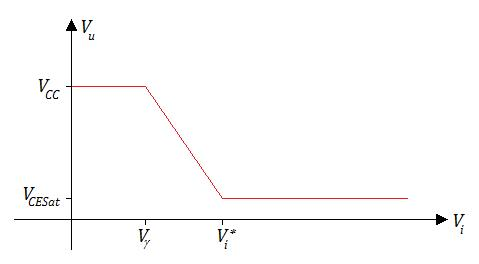
\includegraphics[scale=0.45]{78.png}
			\caption{Caratteristica ingresso-uscita dell’invertitore RTL}
			\label{fig:im-78}
		\end{figure}
	\end{center}
	Il ramo di caratteristica nella regione di interdizione è ovviamente identico a quanto visto senza la resistenza $R_B$. \\
	Tale resistenza è infatti inserita per limitare la corrente ma a transistore spento la corrente è nulla e dunque la resistenza $R_B$ non interviene.\\\\
	Nella regione normale l’uscita è rappresentata da una retta. \\
	Se l’approssimazione del modello fosse buona, otterremmo un grande vantaggio da questa caratteristica poiché consentirebbe di gestire facilmente l’amplificazione dal momento che una amplificazione lineare non distorce il segnale ricevuto.\\\\
	Dalle simulazione svolte al calcolatore sul dispositivo reale possiamo notare che l’andamento ottenuto dal modello a soglia è qualitativamente identico all’andamento della caratteristica ingresso-uscita del dispositivo reale.\\\\
	Il circuito in Figura \ref{fig:im-77} è detto Invertitore RTL (\textbf{Resistor Transistor Logic}, logica a transistore e resistore) ed è un circuito fuzionante.\\\\
	Eventualmente anche le sezioni degli appunti: "3.16 – Qualità dell'invertitore RTL", "3.22,3.23 – Rete di invertitori e Fan-Out" e "6.1 – Esempio 1"
%************************************************************************************************************************************************************************************
	\section{Margini di immunità ai disturbi}
	\subsection{Qualità dell'invertitore RTL}
	Nella sezione \ref{sub:inv-rtl} abbiamo dimostrato che il circuito di Figura \ref{fig:im-77} rappresenta un invertitore. \\
	Vogliamo ora studiarne la qualità.
	\subsubsection{Invertitore}
	Prima di tutto è necessario accertarci che il circuito sia effettivamente un invertitore logico. \\
	Infatti, scelti due valori:
	$$\begin{cases} V_L = V_{CESat} \\ V_H = V_{CC} \end{cases}$$
	mentre per il valore $V_{CESat}$ siamo certi che esso sia minore di $V_\gamma$, per il valore alto $V_{CC}$ non sappiamo se valga:
	$$V_{CC} > V_i^*$$
	Questa condizione è vera solo quando abbiamo:
	$$|A_V| > \frac{V_{CC} - V_{CESat}}{V_{CC} - V_\gamma}$$
	che, fortunatamente, non è un vincolo critico. \\
	Questo risultato, però, mostra che, anche per avere un invertitore, dobbiamo avere un guadagno elevato.
	\subsubsection{Resistenza ai disturbi (Effeto del rumore)}
	\label{subsub:res-dist}
	Una volta assicuratici di disporre di un invertitore logico, dobbiamo controllarne la resistenza ai disturbi in modo da poterlo effettivamente utilizzare in una rete logica o come amplificatore.\\\\
	Possiamo interpretare il rumore come una piccola variazione rispetto al segnale che si desidera rappresentare. \\
	L’effetto di questa variazione è estremamente diverso in base alla regione in cui si lavora.
	\paragraph{Segnale analogico}
	Il segnale analogico sfrutta il tratto ad elevata pendenza della caratteristica.
	$$|A_V| = \frac{dV_u}{dV_i} = \lim_{\Delta V_i \rightarrow 0} \frac{\Delta V_u}{\Delta V_i} > 1$$
	Inoltre, per quanto riguarda i segnali analogici, una delle ipotesi fondamentali formulate all’inizio dell’analisi del BJT, era quella di piccolo scostamento.\\\\
	In presenza di rumore allora l’amplificatore amplifica sia il segnale analogico ricevuto sia il rumore rendendo di fatto indistinguibile la variazione dell’uscita voluta (cioè quella associata al segnale) da quella non voluta (cioè quella associata al rumore).
	\paragraph{Segnale digitale}
	Il segnale digitale sfrutta i tratti a pendenza quasi nulla.
	$$|A_V| = \frac{dV_u}{dV_i} = \lim_{\Delta V_i \to 0} \frac{\Delta V_u}{\Delta V_i} = 0$$
	In questo caso, un rumore che scosti di poco il segnale di ingresso dal suo valore nominale non provoca variazioni significative sul valore di uscita.\\\\
	La rete digitale è allora più immune ai disturbi rispetto all’amplificatore poiché è in grado di distinguere il segnale dal rumore. \\
	Il circuito di Figura \ref{fig:im-77} allora funziona meglio come circuito digitale rispetto a quanto può fare come amplificatore.
	\subsubsection{Immunità ai disturbi}
	\paragraph{Valori fondamentali}
	Abbiamo scoperto che l’invertitore RTL è in grado, quando usato come porta logica binaria, di discriminare tra il segnale ed il rumore. \\
	Questa discriminazione è fattibile solo quando il rumore (indicato con $N$ per noise) non supera una certa ampiezza. \\
	Cioè vogliamo individuare il massimo valore di $N$ tale per cui sia
	$$V_i^{**} = V_L + N \longrightarrow V_u = V_H$$
	Dalla caratteristica possiamo facilmente individuare il valore massimo del rumore come:
	$$N_{Max} = V_i^{**} - V_L$$
	Ancora dalla caratteristica possiamo identificare facilmente tale valore limite come $V_\gamma$. In generale indicheremo tale punto con:
	$$V_{iL \ Max}$$
	e quindi possiamo ricavare:
	$$N_{Max} = V_{iL \ Max} - V_L$$
	che nel nostro caso specifico, con valori tipici di, è:
	$$N_{Max} = V_\gamma - V_{CESat} = 0,75 - 0,2 = 0,55\ \text{V}$$
	Analogamente possiamo individuare un valore di rumore tale da non modificare l’uscita quando in ingresso abbiamo $V_H$.
	$$V_i^{***} = V_H + N \longrightarrow V_u = V_L$$
	Di nuovo, dalla caratteristica, ricaviamo che il massimo rumore sovrapponibile a $V_H$ è:
	$$N_{Max} = V_{iH \ Min} = V_\gamma + \frac{V_{CC} - V_{CESat}}{|A_V|}$$
	$$N_{Max} = V_H - V_i^* = V_{CC} - V_\gamma - \frac{V_{CC} - V_{CESat}}{|A_V|} = 3,77\ \text{V}$$
	Si nota che questo margine dipende dal guadagno. \\
	Maggiore è il guadagno, maggiore è l’immunità ai disturbi per il valore alto.\\\\
	Possiamo inoltre identificare l’escursione (\textbf{Logic Swing}) come:
	$$\Delta V_u = V_H - V_L$$
	ed il massimo errore tollerabile rispetto al valore basso come:
	$$N_{ML} = V_{iL \ Max} - V_L$$
	mentre per il valore alto è:
	$$N_{MH} = V_H - V_{iH \ Min}$$
	Con i valori tipici notiamo che $N_{ML}$ è significativamente più piccolo rispetto a $N_{MH}$. \\
	In fase di progetto dovremo allora considerare $N_{ML}$ come parametro di resistenza. In generale sarà:
	$$N_M = \min \left\{N_{ML}, N_{MH}\right\}$$
	Imponendo che entrambi i margini siano positivi e facendo la somma delle due relazioni otteniamo:
	$$N_{MH} + N_{ML} = V_H - V_{iH \ Min} + V_{iL \ Max} - V_L > 0$$
	da cui possiamo ricavare:
	$$\underbrace{V_H - V_L}_{\Delta V_u} > \underbrace{V_{iH \ Min} - V_{iL \ Max}}_{\Delta V_i}$$
	Ma $V_H - V_L$ è l’escursione mentre $V_{iH \ Min} - V_{iL \ Max}$ è l’escursione dell’ingresso. \\
	Allora:
	$$\frac{\Delta V_u}{\Delta V_i} > 1 \implies |A_V| > 1$$
	e quindi, per avere un buon invertitore, dobbiamo necessariamente realizzare un buon amplificatore. \\
	La Figura \ref{fig:im-82} mostra graficamente i margini appena individuati.\\\\
	Siccome la somma tra $N_{ML}$ e $N_{MH}$ è limitata, se aumentiamo uno, l’atro deve diminuire. \\
	La condizione ottima di progetto (Figura \ref{fig:im-83}) è:
	$$N_{ML} = N_{MH}$$
	\begin{figure}[h]
		
		\begin{subfigure}{0.5\textwidth}
			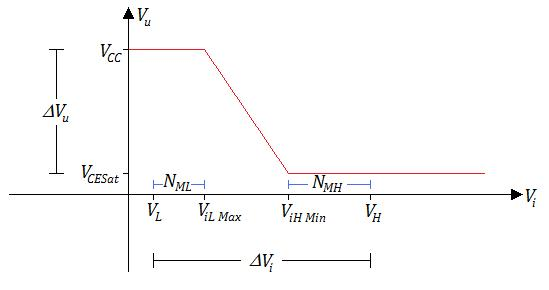
\includegraphics[width=0.9\linewidth]{82.png} 
			\caption{Rappresentazione grafica dei margini di immunità ai disturbi}
			\label{fig:im-82}
		\end{subfigure}
		\begin{subfigure}{0.5\textwidth}
			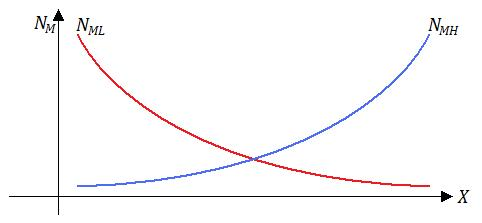
\includegraphics[width=0.9\linewidth]{83.png}
			\caption{La condizione ottima di progetto consiste nell’individuazione del miglior equilibrio possibile tra $N_{ML}$ e $N_{MH}$}
			\label{fig:im-83}
		\end{subfigure}
		
		\caption{}
		\label{fig:image10}
	\end{figure}
	\paragraph{Esempio Pratico}
	Consideriamo il circuito di Figura \ref{fig:im-84} e cerchiamo di individuarne l’immunità ai disturbi.
	\begin{center}
		\begin{figure}[h]
			\centering
			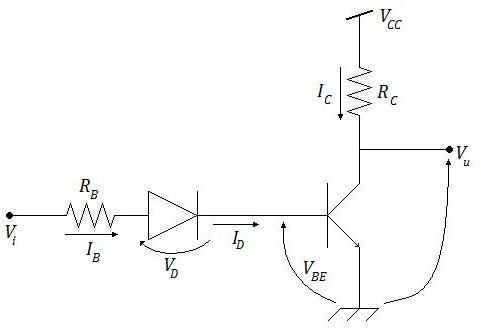
\includegraphics[scale=0.45]{84.png}
			\caption{L’aggiunta del diodo aumenta l’immunità ai disturbi della rete}
			\label{fig:im-84}
		\end{figure}
	\end{center}
	Dal momento che in serie alle giunzioni abbiamo un caricoresistivo possiamo utilizzare i modelli a soglia. \\
	Per ridurre le regioni di studio, osserviamo preliminarmente che:
	$$I_D = I_B$$
	Allora se il diodo è acceso deve valere:
	$$I_D > 0 \Longrightarrow I_B > 0$$
	e quindi il transistore deve essere acceso. Parimenti, se il transistore è acceso, il diodo non può essere spento. \\
	Allora dobbiamo valutare solo tre casi contro i sei indicati dal modello a soglia.
	\subparagraph{Regione di interdizione}
	In questa regione è:
	$$\begin{cases} I_C = 0 \\ V_u = V_{CC} - R_C I_C \end{cases} \quad \Longrightarrow V_u = V_{CC} $$
	$$ \begin{cases} V_{BE} < V_\gamma \\ V_D < V_\gamma \end{cases}$$
	$$\begin{cases} V_i - R_B I_B - V_D - V_{BE} = 0 \\ I_B = 0 \end{cases} \implies V_i < 2V_\gamma$$
	\subparagraph{Regione normale} 
	In regione normale abbiamo:
	$$\begin{cases} V_{BE} > V_\gamma \\ V_D > V_\gamma \end{cases}$$
	$$\begin{cases} I_B = \frac{V_i - 2V_\gamma}{R_B} \\ I_C = \beta_F I_B \\ V_u = V_{CC} - R_C I_C \end{cases} \implies V_u = V_{CC} - \frac{\beta_F R_C}{R_B} (V_i - 2V_\gamma)$$
	La $V_u$ è una retta della stessa pendenza della retta del circuito di Figura \ref{fig:im-77}. \\
	Tale tratto si estende in:
	$$2V_\gamma < V_i < 2V_\gamma + \frac{V_{CC} - V_{CESat}}{|A_V|}$$
	\subparagraph{Regione di saturazione} 
	In questo caso, ovviamente è:
	$$\begin{cases} V_u = V_{CESat} \\ V_i > V_i^* \end{cases}$$
	dove:
	$$V_i^* = 2V_\gamma + \frac{V_{CC} - V_{CESat}}{|A_V|}$$
	\subparagraph{Considerazioni finali} 
	La caratteristica è perfettamente identica alla caratteristica del circuito di Figura \ref{fig:im-77} ma è stata traslata in avanti di $V_\gamma$. \\
	Allora i margini si sono spostati. \\
	Risultano infatti:
	$$N_{ML} = 2V_\gamma - V_{CESat} = 1,3 \text{ V}$$
	$$N_{MH} = V_{CC} - 2V_\gamma - \frac{V_{CC} - V_{CESat}}{|A_V|} = 2,02 \text{ V}$$
	$$N_M = 1,3 \text{ V}$$
	L’aggiunta del diodo ha quindi più che raddoppiato il margine di resistenza al rumore. \\
	In linea di principio possiamo pensare di aggiungere diodi per spostare la caratteristica. \\
	Queste soluzioni sono praticate ma senza portarle a conseguenze estreme: l’aggiunta di troppi diodi infatti provoca un peggioramento delle prestazioni dinamiche.
%************************************************************************************************************************************************************************************
	\section{Effetti reattivi BJT e modello a controllo di carica}
	\subsection{Modello dinamico del BJT}
	Abbiamo ormai concluso lo studio della caratteristica statica dell'invertitore RTL.\\
	Vogliamo ora valutare la risposta dinamica dell'invertitore.\\
	Per il diodo avevamo sviluppato un modello a soglia, detto \textit{modello a controllo di carica}, descritto da:
	\[ \begin{cases} V < V_\gamma & \begin{cases} I_D = 0 \\ Q \approx 0 \end{cases} \\ V = V_\gamma & \begin{cases} I_D > 0 \\ Q > 0 \end{cases} \end{cases} \]
	\[ I_D = \frac{Q}{\tau} = \frac{Q_S \left( e^{\frac{V}{V_T}} - 1 \right)}{\tau} \]
	Siccome il transistore bipolare è costituito da due diodi, possiamo sfruttare nuovamente quanto visto per il diodo.\\
	Dal modello dei due diodi abbiamo definito il modello di Ebers \& Moll.
	\[ \begin{cases} I_B = I_{BES} \left( e^{\frac{V_{BE}}{V_T}} - 1 \right) + I_{BCS} \left( e^{\frac{V_{BC}}{V_T}} - 1 \right) \\ I_C = I_S \left( e^{\frac{V_{BE}}{V_T}} - 1 \right) - (I_{BCS} + I_S) \left( e^{\frac{V_{BC}}{V_T}} - 1 \right) \\ I_E = (I_{BES} + I_S) \left( e^{\frac{V_{BE}}{V_T}} - 1 \right) - I_S \left( e^{\frac{V_{BC}}{V_T}} - 1 \right) \end{cases} \]
	Dal modello abbiamo poi ricavato versioni semplificate per le tre zone di polarizzazione possibili.
	\subsubsection{Polarizzazione diretta}\label{par:19.4.1}
	Dallo studio delle singole zone di funzionamento si nota che in regione normale sia la corrente $I_C$ sia la carica $Q_F$ dipendono in maniera esponenziale dalla $V_{BE}$.
	\[ \begin{cases} I_C = I_F \left( e^{\frac{V_{BE}}{V_T}} - 1 \right) \\ Q_F = Q_B \left( e^{\frac{V_{BE}}{V_T}} - 1 \right) \end{cases} \quad \Rightarrow \frac{Q_F}{I_C} = \frac{Q_B}{I_B} = \tau_F \]
	\[ Q_F = \tau_F I_C \]
	Allora possiamo generalizzare il modello esattamente come abbiamo fatto per il diodo.
	\[ \begin{cases} I_C = \frac{Q_F}{\tau_F} \\ I_E = \frac{I_C}{\alpha_F} = \frac{Q_F}{\alpha_F \tau_F} \\ I_B = I_E - I_C = \frac{Q_F}{\alpha_F \tau_F} - \frac{Q_F}{\tau_F} = \frac{Q_F}{\beta_F \tau_F} \end{cases} \]
	Il grafico del modello dinamico a controllo di carica del BJT per la regione normale è riportato in Figura \ref{fig:im-96}.
	\begin{center}
		\begin{figure}[h]
			\centering
			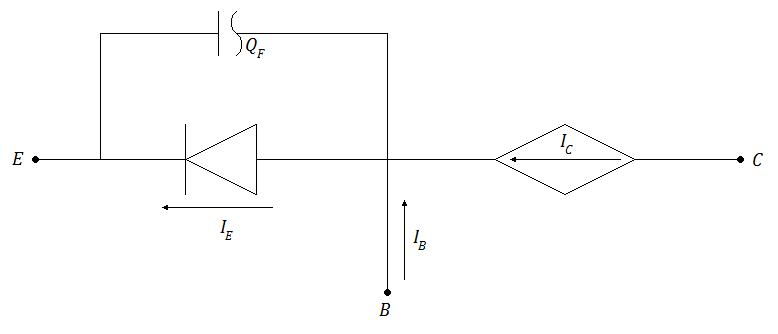
\includegraphics[scale=0.45]{96.png}
			\caption{Modello dinamico della polarizzazione diretta del BJT.}
			\label{fig:im-96}
		\end{figure}
	\end{center}
	\subsubsection{Polarizzazione inversa}
	Ragionando in modo analogo a quanto fatto nel Paragrafo \ref{par:19.4.1}, e ricordando che in inversa si scambiano di ruolo collettore ed emettitore, ricaviamo:
	\[ Q_R = Q_{RS} \left( e^{\frac{V_{BC}}{V_T}} - 1 \right) \]
	\[ Q_F = \tau_F I_C \]
	Allora possiamo generalizzare il modello esattamente come abbiamo fatto per il diodo.
	\[ \begin{cases} I_E = \frac{Q_R}{\tau_R} \\ I_C = \frac{Q_R}{\alpha_R \tau_R} \\ I_B = \frac{Q_B}{\beta_R \tau_R} \end{cases} \]
	Il grafico è riportato in Figura \ref{fig:im-97}.
	\begin{center}
		\begin{figure}[h]
			\centering
			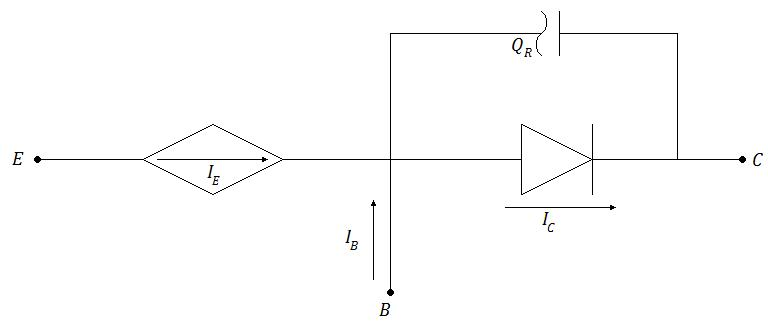
\includegraphics[scale=0.45]{97.png}
			\caption{Modello dinamico della polarizzazione inversa del BJT.}
			\label{fig:im-97}
		\end{figure}
	\end{center}
	\subsubsection{Regione di saturazione}
	Si tratta del modello più generale possibile.\\
	Come già il modello statico è ricavabile facilmente dalla somma dei modelli per la polarizzazione diretta ed inversa.\\\\
	Il grafico è riportato in Figura \ref{fig:im-98}.
	\begin{center}
		\begin{figure}[h]
			\centering
			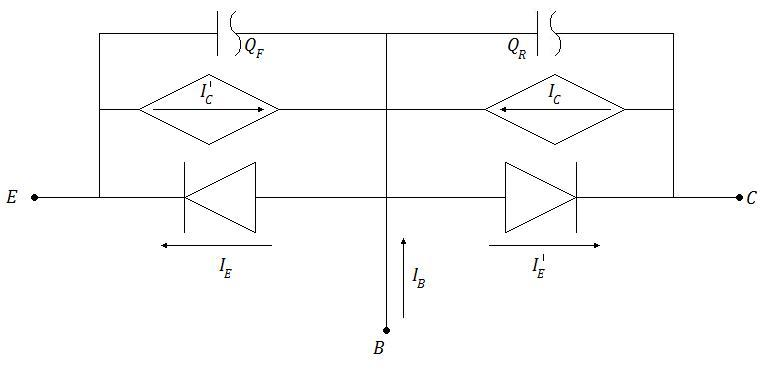
\includegraphics[scale=0.45]{98.png}
			\caption{Modello dinamico della regione di saturazione del BJT. \\ I termini indicati con $I_x'$ sono relativi alla polarizzazione inversa mentre i termini $I_x$ sono relativi alla polarizzazione diretta.}
			\label{fig:im-98}
		\end{figure}
	\end{center}
	\subsubsection{Modello dinamico}\label{par:20.2}
	Il modello dinamico è riportato in Figura \ref{fig:im-98}.
	Le equazioni che descrivono tale modello sono:
	\[ \begin{cases} Q_F = Q_{FS} \left( e^{\frac{V_{RE}}{V_T}} - 1 \right) \\ Q_R = Q_{RS} \left( e^{\frac{V_{RC}}{V_T}} - 1 \right) \end{cases} \]
	\[ \begin{cases} I_C = \frac{Q_F}{\tau_F} \\ I'_C = \frac{Q_R}{\tau_R} \end{cases}\]
	\[\begin{cases} I_E = \frac{Q_F}{\alpha_F \tau_F} \\ I'_E = \frac{Q_R}{\alpha_R \tau_R} \end{cases}\]
	\[I_B = \frac{Q_F}{\beta_F \tau_F} \cdot \frac{Q_R}{\beta_R \tau_R}\]
	Possiamo inoltre vedere ogni corrente come somma o differenza delle altre correnti:
	\[ \left\{ \begin{array}{l} I_C = \frac{Q_F}{\tau_F} - \frac{Q_R}{\alpha_R \tau_R} - \frac{dQ_R}{dt} \\ I_E = \frac{Q_F}{\alpha_F \tau_F} - \frac{Q_R}{\tau_R} + \frac{dQ_F}{dt} \\ I_B = \frac{Q_F}{\beta_F \tau_F} + \frac{Q_R}{\beta_R \tau_R} + \frac{dQ_F}{dt} + \frac{dQ_R}{dt} \end{array} \right. \]
	\subsection{Risposta dinamica} \label{sub:risposta-dinamica}
	Sfruttiamo ora il modello riportato nel Paragrafo \ref{par:20.2} e calcoliamo la risposta dinamica di un invertitore RTL con fan out pari a zero (Figura \ref{fig:im-99}).
	\begin{center}
		\begin{figure}[h]
			\centering
			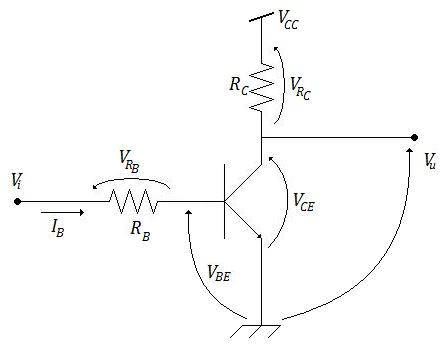
\includegraphics[scale=0.45]{99.png}
			\caption{Invertitore RTL con fan out pari a zero.}
			\label{fig:im-99}
		\end{figure}
	\end{center}
	Supponiamo di mandare in ingresso un segnale variabile nel tempo simile a quello riportato in Figura \ref{fig:im-100}.
	\begin{center}
		\begin{figure}[h]
			\centering
			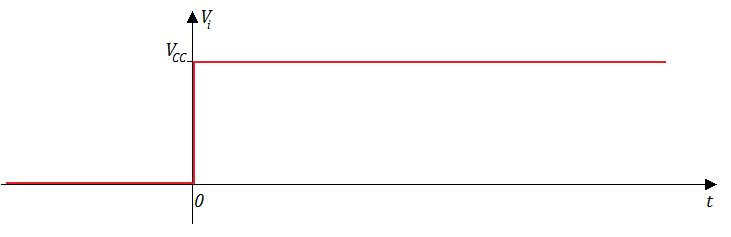
\includegraphics[scale=0.45]{100.png}
			\caption{Segnale a gradino in ingresso per lo studio della risposta dinamica dell'invertitore RTL.}
			\label{fig:im-100}
		\end{figure}
	\end{center}
	Siccome sia $Q_F$ sia $Q_R$ sono descritte da funzioni esponenziali di difficile gestione, sfruttiamo le opportune approssimazioni (riportate in Figura \ref{fig:im-101}).
	\begin{center}
		\begin{figure}[h]
			\centering
			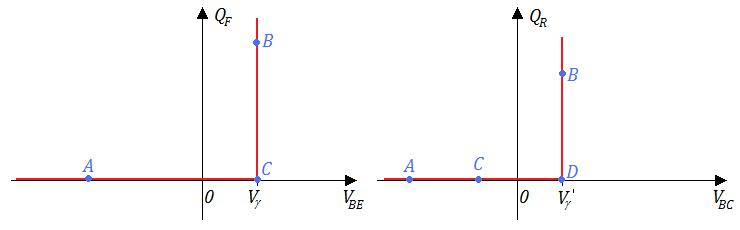
\includegraphics[scale=0.45]{101.png}
			\caption{Modelli a soglia di $Q_F$ e $Q_R$. Sono evidenziati i punti notevoli studiati nel seguito.}
			\label{fig:im-101}
		\end{figure}
	\end{center}
	\subsubsection{Situazione per $t < 0$ (punto A)}
	In questa situazione siamo in una condizione statica.\\
	Allora possiamo riprendere l'analisi statica già svolta.\\
	Siccome è $V_i = 0$, il transistore è spento (in interdizione).\\
	Allora è:
	\[ V_u = V_{CC} \]
	\[ I_B = 0 \implies \frac{V_i - V_{BE}}{R_B} = 0 \implies V_i = V_{BE} = 0 \]
	Allora, grazie alle approssimazioni di Figura \ref{fig:im-101}, possiamo dire che $Q_F$ è nulla.\\
	Inoltre:
	\[ V_{CC} - V_u = 0 \implies V_u = V_{CC} \implies V_{BC} = V_{BE} - V_{CE} = -V_{CC} \]
	dimostra che anche $Q_R$ è nulla.
	\subsubsection{Situazione per $t \rightarrow +\infty$ (punto B)}
	Per $t > 0$ l'ingresso si porta a $V_{CC}$.\\
	Per un tempo sufficientemente lungo, torniamo poi nella situazione già studiata nel caso statico.\\
	Allora è:
	\[ V_u = V_{CESat} \]
	da cui segue che deve essere:
	\[ \begin{cases} V_{BE} = V_\gamma \\ V_{BC} = V_\gamma' \end{cases} \implies \begin{cases} Q_F \geq 0 \\ Q_R \geq 0 \end{cases} \]
	Dalle equazioni del modello possiamo inoltre ricavare:
	\[ \begin{cases} I_C = \frac{Q_F}{\tau_F} + \frac{Q_R}{\alpha_R \tau_R} = \frac{V_{CC} - V_{CESat}}{R_C} \\ I_B = \frac{Q_F}{\tau_{BF}} + \frac{Q_R}{\tau_{BR}} = \frac{V_{CC} - V_\gamma}{R_B} \end{cases} \]
	dove abbiamo assunto $\tau_{BF} \doteq \beta_F \tau_F$ e $\tau_{BR} \doteq \beta_R \tau_R$.\\
	Sostituendo possiamo ottenere:
	\[ I_B = \frac{1}{\tau_F} \cdot \left( I_C + \frac{Q_R}{\alpha_R \tau_R} \right)  \frac{Q_R}{\beta_R \tau_R} \] 
	da cui isoliamo: 
	\[ Q_R = \tau_R \cdot \frac{\beta_F I_B - I_C}{\frac{1}{\alpha_R} + \frac{\beta_F}{\beta_R}} = K \cdot (\beta_F I_B - I_C) > 0 \]
	Analogamente, possiamo ricavare che anche $Q_F$ è maggiore di zero.
	\subsubsection{Situazione per $t > 0$ (punti C e D)}\label{par:20.3.3}
	Dalle due condizioni asintotiche notiamo che la situazione è simile a quella già vista per il diodo: la carica si dovrà spostare dal tratto orizontale al tratto verticale.\\
	Per mantenere la generalità della trattazione dovremo considerare che $Q_F$ e $Q_R$ passiamo per i punti C e D in momenti differenti.\\\\
	L'ingresso commuta istantaneamente e si porta a:
	\[ V_i = V_{CC} \]
	Nel tratto da A a C, abbiamo:
	\[ \begin{cases} Q_F = 0 \\ V_{BE} = V_\gamma \end{cases} \]
	che, siccome non si ha spostamento di carica, è un transitorio istantaneo.\\
	Allora, istantaneamente, si passa a:
	\[ I_B = \frac{V_{CC} - V_\gamma}{R_B} \]
	La corrente di collettore è invece:
	\[ I_C = \frac{Q_F}{\tau_F} - \underbrace{\frac{Q_R}{\alpha_R \tau_R}}_{=0} - \underbrace{\frac{dQ_R}{d\tau}}_{=0} \]
	ed allora la tensione di uscita è:
	\[ V_u = V_{CC} - R_C I_C = V_{CC} - R_C \cdot \frac{Q_F}{\tau_F} \]
	Allora per avere $V_u = V_{CESat}$ è necessario che $Q_F$ sia maggiore di zero.\\
	Dunque prima si accende la giunzione base-emettitore e poi si accende anche la giunzione collettore-emettitore.\\\\
	Riassumendo possiamo suddividere il transitorio in tre parti:
	\begin{enumerate}
		\item da $\mathbf{A}$ a $\mathbf{C}$ (le cariche sono entrambé nulle)
		\item da \(\mathbf{C}\) a \(\mathbf{D}\) \((Q_{F} > 0\text{ e }Q_{R} = 0)\)
		\item da $\mathbf{D}$ a $\mathbf{B}$ (entrambe le cariche sono positive)
	\end{enumerate}
	\paragraph{Tratto 1}
	In questo transitorio abbiamo:
	\[ \begin{cases} V_{BE} < V_\gamma \\ V_{BC} < V_\gamma' \end{cases} \]
	Dal momento che questo transitorio è istantaneo non è riportato nei grafici.
	\paragraph{Tratto 2}\label{par:20.3.3.2}
	In questo transitorio abbiamo:
	\[ \begin{cases} V_{BE} = V_\gamma \\ V_{BC} < V_\gamma' \end{cases} \]
	La corrente di base è esprimibile come:
	\[ I_B = \frac{V_{CC} - V_\gamma}{R_B} = \frac{Q_F}{\tau_{BF}} + \frac{dQ_F}{dt} \]
	\[ \frac{dQ_F}{dt} = I_B - \frac{Q_F}{\tau_{BF}} \implies \frac{dQ_F}{Q_F - \tau_{BF} I_B} = -\frac{dt}{\tau_{BF}} \]
	che, integrata, porta a:
	\[ -\frac{t}{\tau_{BF}} = \ln \frac{Q_F(t) - \tau_{BF} I_B}{-\tau_{BF} I_B} \implies e^{-\frac{t}{\tau_{BF}}} = \frac{Q_F(t) - \tau_{BF} I_B}{-\tau_{BF} I_B} \]
	da cui ricaviamo:
	\[ Q_F(t) = \tau_{BF} I_B \left( 1 - e^{-\frac{t}{\tau_{BF}}} \right) \]
	che è l'andamento di un esponenziale crescente nel tempo.\\\\
	La carica $Q_R$ in questo tratto è ancora nulla.\\\\
	L'uscita è:
	\[ V_u(t) = V_{CC} - \frac{R_C}{\tau_F} \cdot \frac{\beta_F \tau_F}{R_B} \cdot (V_{CC} - V_\gamma) \cdot \left( 1 - e^{-\frac{t}{\tau_{BF}}} \right) \]
	è un esponenziale decrescente.\\
	L'uscita mantiene questo andamento fino a quando non raggiunge il valore $V_{CESat}$.\\
	Il tempo $t_F$ tale che sia:
	\[ V_u(t_F) = V_{CESat} \]
	è detto \textit{tempo di discesa} (\textit{fall}).
	\paragraph{Tratto 3}
	In questo ultimo tratto del transitorio abbiamo:
	\[ \begin{cases} V_{BE} = V_\gamma \\ V_{BC} = V_\gamma' \end{cases} \]
	\[ V_{CE} = V_u = V_{CESat} \]
	Dal punto di vista del valore dell'uscita allora il transitorio è finito.\\
	Resta però da valutare il transitorio dello spostamento delle cariche $Q_F$ e $Q_R$.\\
	Questa volta però il modello non può essere semplificato.\\
	Siccome siamo in saturazione il modello è descritto come:
	\[ \begin{cases} I_C = \frac{V_{CC} - V_\gamma}{R_B} = \frac{Q_F}{\tau_F} - \frac{Q_R}{\alpha_R \tau_R} - \frac{dQ_R}{dt} \\ I_B = \frac{V_{CC} - V_{CESat}}{R_C} = \frac{Q_F}{\beta_F \tau_F} + \frac{Q_R}{\beta_R \tau_R} + \frac{dQ_F}{dt} + \frac{dQ_R}{dt} \end{cases} \]
	che, risolto, porta nuovamente a degli esponenziali.
	\subsubsection{Transitorio di spegnimento}
	Consideriamo ora di tornare indietro: l'ingresso commuta dal valore alto al valore basso.\\
	Il transitorio può essere ora suddiviso in altri tre tratti, opposti a quelli esaminati nel Paragrafo \ref{par:20.3.3}:
	\begin{enumerate}
		\item da \textbf{B} a \textbf{D} (sia $Q_F$ sia $Q_R$ sono positive)
		\item da \textbf{D} a \textbf{C} ($Q_R = 0$ e $Q_F > 0$)
		\item da \textbf{C} a \textbf{A} (sia $Q_F$ sia $Q_R$ sono nulle)
	\end{enumerate}
	\paragraph{Tratto 1}
	In questo caso abbiamo:
	\[ \begin{cases} V_i = 0 \\ V_{BE} = V_\gamma \\ I_B = \frac{V_i - V_{BE}}{R_B} \end{cases} \implies I_B = -\frac{V_\gamma}{R_B} \]
	da cui segue che l'uscita è:
	\[ \begin{cases} V_{BE} = V_\gamma \\ V_{BC} = V_\gamma' \end{cases} \implies V_{CE} = V_{CESat} = V_u \]
	\paragraph{Tratto 2}
	In questo caso è:
	\[ V_{BE} = V_\gamma \implies I_B = -\frac{V_\gamma}{R_B} \]
	Siccome possiamo ora semplificare nuovamente l'espressione di $I_B$ possiamo trovare la stessa espressione del Paragrafo \ref{par:20.3.3.2} con l'unica differenza che il termine noto passa da un valore positivo ad un valore negativo.\\\\
	Allora mentre la carica $Q_F$ cala fino al valore nullo, la tensione di uscita tende a salire verso il valore $V_{CC}$.\\\\
	Si noti che la corrente di scarica $I_B$ è significativamente più piccola rispetto alla corrente di carica.\\
	Allora, tipicamente, il tempo di salita $t_R$ (\textit{rise}) è significativamente più elevato rispetto al tempo di caduta.
	\paragraph{Tratto 3}
	Nuovamente si tratta di un transitorio istantaneo poiché non vi è alcuno spostamento di carica.
	\subsubsection{Grafici e considerazioni finali}
	La Figura \ref{fig:im-102} riporta tutti i valori fondamentali.
	\begin{center}
		\begin{figure}[h]
			\centering
			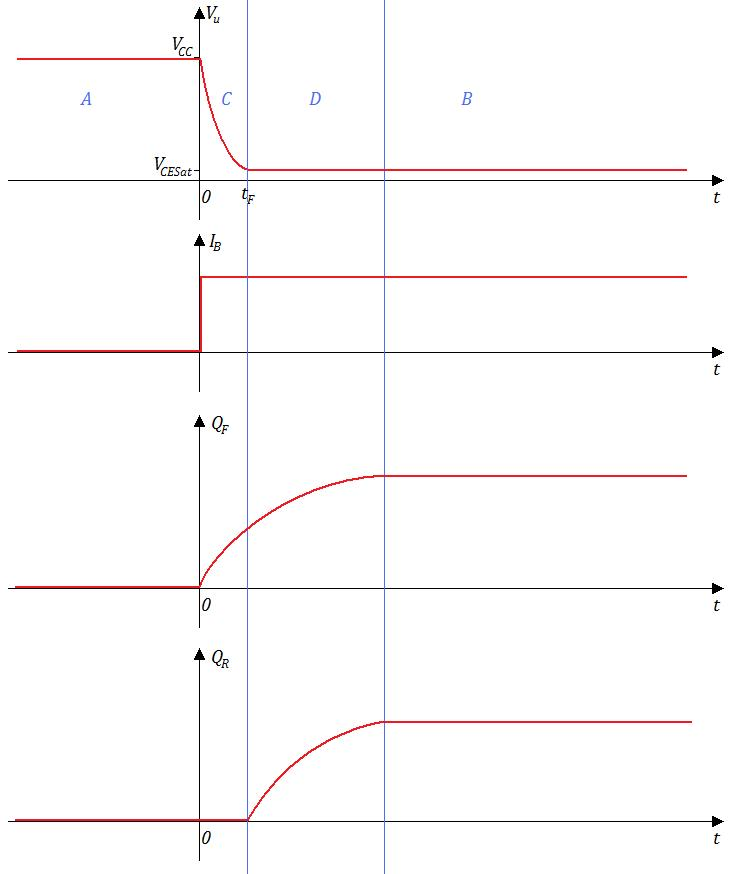
\includegraphics[scale=0.45]{102.png}
			\caption{Grafici di $V_u$, $I_B$, $Q_F$ e $Q_R$ della risposta dinamica.}
			\label{fig:im-102}
		\end{figure}
	\end{center}
	La Figura \ref{fig:im-103} mostra l'andamento dell'ingresso e dell'uscita.
	\begin{center}
		\begin{figure}[h]
			\centering
			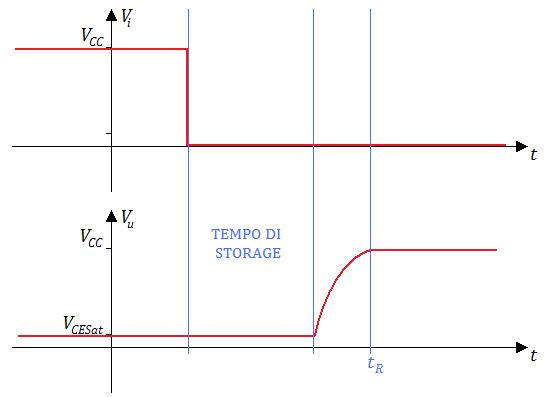
\includegraphics[scale=0.45]{103.png}
			\caption{Transitorio dello spegnimento dell'invertitore RTL. \\ Si nota che la variazione della tensione di uscita è lenta anche a causa del tempo di storage.}
			\label{fig:im-103}
		\end{figure}
	\end{center}
	Ancora una volta abbiamo una risposta fortemente asimmetrica: l'accensione è molto più rapida dello spegnimento (ove incidono sia il tempo di storage sia la corrente più bassa).\\
	Il tempo di storage è a sua volta determinato dalla carica $Q_R$.
	\[ \begin{cases} Q_R = K \cdot (\beta_F I_B - I_C) \\ I_B = \frac{V_{CC} - V_\gamma}{R_B} \\ I_C = \frac{V_{CC} - V_{CESat}}{R_C} \end{cases} \]
	La carica $Q_R$ allora è tanto più elevata quanto più elevato è il guadagno a vuoto del dispositivo.
	\[ \frac{\beta_F R_C}{R_B} \cdot \frac{V_{CC} - V_\gamma}{V_{CC} - V_{CESat}} > 1 \implies |A_V| \cdot \frac{V_{CC} - V_\gamma}{V_{CC} - V_{CESat}} > 1 \]
	Dunque, in fase di progetto, si dovrà tenere conto di questo fatto e cercare di ottenere un buon compromesso.\\
	Abbasando il guadagno, riduciamo il tempo di salita ma abbassiamo sia il margine di immunità ai disturbi sia il fan out massimo sopportabile.
%************************************************************************************************************************************************************************************
	\section{Transitori di commutazione RTL}
	Per questa risposta fare riferimento a \ref{sub:risposta-dinamica}
%************************************************************************************************************************************************************************************
	\section{JFET: principi di funzionamento}
	\subsection{Transistori ad effetto di campo}
	Consideriamo un blocco di materiale uniformemente drogato di tipo $n$ con una concentrazione $N = N_D$ (Figura \ref{fig:im-115}).\\
	La conducibilità di questo dispositivo è:
	$$\sigma = q\mu_n N = q\mu_n N_D$$
	All'applicazione di un campo elettrico $\bar{E}$ avremo una corrente:
	$$\bar{J} = \sigma \bar{E}$$
	ed allora il blocchetto si caratterizza come una resistenza data da:
	$$R = \frac{1}{\sigma} \cdot \frac{L}{wh}$$
	\begin{center}
		\begin{figure}[h]
			\centering
			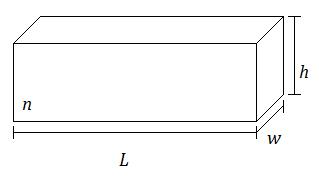
\includegraphics[scale=0.45]{115.png}
			\caption{Un blocchetto di semiconduttore.}
			\label{fig:im-115}
		\end{figure}
	\end{center}
	Consideriamo ora la giunzione $p_n$ ed applichiamo una differenza di potenziale $V$ (Figura \ref{fig:im-116}).\\\\
	Nelle regioni neutre la conducibilità sarà ancora:
	$$\begin{cases} \sigma_n = q\mu_n N_D \\ \sigma_p = q\mu_p N_A \end{cases}$$
	mentre per entrambe le regioni svuotate la conducibilità sarà nulla.
	\begin{center}
		\begin{figure}[h]
			\centering
			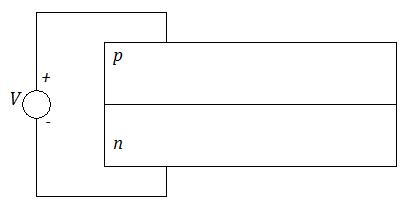
\includegraphics[scale=0.45]{116.png}
			\caption{Giunzione $p_n$ a cavallo della quale si applica una differenza di potenziale $V$.}
			\label{fig:im-116}
		\end{figure}
	\end{center}
	Costruiamo un nuovo dispositivo con le due considerazioni sopra riportate.\\
	Il dispositivo (Figura \ref{fig:im-117}) consiste in una giunzione $p_n$ a cavallo della quale è posto un generatore di tensione $V_2$.\\
	Sulla porzione drogata $n$ si applica un generatore di tensione $V_1$.\\
	La portata massima della corrente circolante sul dispositivo è pari al volume massimo della regione drogata $n$.\\
	In genere avremo:
	$$R = \frac{1}{q\mu_n N_D} \cdot \frac{L}{w(h - w(V))}$$
	dove $w(V)$ è la dimensione della regione svuotata al variare della tensione data da $V_2$.
	\begin{center}
		\begin{figure}[h]
			\centering
			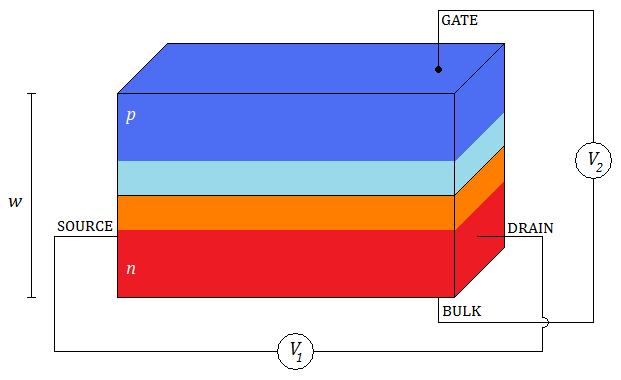
\includegraphics[scale=0.45]{117.png}
			\caption{Un JFET.}
			\label{fig:im-117}
		\end{figure}
	\end{center}
	Questo dispositivo è detto transistore ad effetto di campo (JFET, \textbf{Junction Field Effect Transistor}) e sfrutta il campo elettrico per modulare la dimensione della regione di canale (che è la regione di conduzione).\\
	Purtroppo un dispositivo di questo tipo è estremamente complesso da realizzare e miniaturizzare.\\\\
	La regione di canale deve poter essere completamente chiusa ma quando abbiamo introdotto la giunzione $p_n$ abbiamo dimostrato che la regione svuotata ha un'ampiezza di pochi micron.\\
	Il chip di silicio ha però uno spessore di centinaia di micron.\\
	Lo svuotamento dell'intero canale allora dovrebbe richiedere tensioni di migliaia di Volt che non sono ragionevoli.\\\\
	Inoltre noi vogliamo poter realizzare circuiti su un solo pezzo di semiconduttore.\\
	Ma due transistori JFET sullo stesso pezzo di semiconduttore possono coesistere solo se circondati da giunzioni $p_n$.\\\\
	I JFET sono allora di difficile utilizzo nei circuiti integrati.\\
	Trovano tuttavia applicazione in campo medico (elettrocardiogramma, elettroencefalogramma, eccetera).
	\subsection{Transistori MOS}
	Nonostante la complessità del JFET l'idea è interessante.\\
	Tale complessità è dovuta alla scelta di modulare le dimensioni fisiche del dispositivo.\\
	Possiamo però modulare anche le caratteristiche di conducibilità.
	Costruiamo un nuovo dispositivo costituito da un semiconduttore (tipicamente il silicio, $Si$), un isolante (l'ossido di silicio, $SiO_2$) ed un conduttore (un metallo).\\
	Un dispositivo di questo tipo è detto transistore MOS (\textbf{Metal Oxide Semiconductor}) ed è una specie di condensatore.
%************************************************************************************************************************************************************************************
	\section{Condensatore MOS}
	\subsection{"Condensatore" MOS (Transistori MOS)}
	Nonostante la complessità del JFET l'idea è interessante.\\
	Tale complessità è dovuta alla scelta di modulare le dimensioni fisiche del dispositivo.\\
	Possiamo però modulare anche le caratteristiche di conducibilità.
	Costruiamo un nuovo dispositivo costituito da un semiconduttore (tipicamente il silicio, $Si$), un isolante (l'ossido di silicio, $SiO_2$) ed un conduttore (un metallo).\\
	Un dispositivo di questo tipo è detto transistore MOS (\textbf{Metal Oxide Semiconductor}) ed è una specie di condensatore.\\
	I transistori MOS (Figura \ref{fig:im-118}) sono attualmente alla base della realizzazione della maggior parte dei circuiti integrati.
	\begin{center}
		\begin{figure}[h]
			\centering
			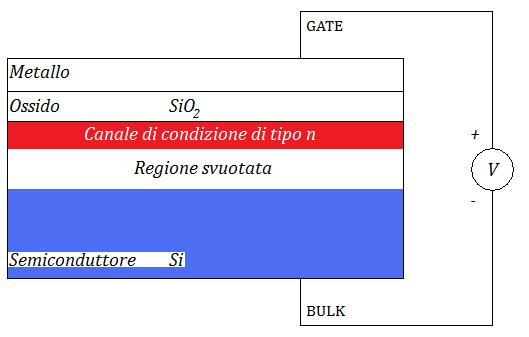
\includegraphics[scale=0.45]{118.png}
			\caption{Un transistore MOS.}
			\label{fig:im-118}
		\end{figure}
	\end{center}
	\subsubsection{Analisi qualitativa}
	Applichiamo una differenza di potenziale $V$ ai capi del dispositivo.\\
	Quando si applica la tensione $V$ gli elettroni del semiconduttore sono trascinati verso l'alto e vengono bloccati contro l'isolante.\\
	Possiamo allora ipotizzare che esista una regione perturbata nei pressi della giunzione tra il semiconduttore e l'isolante dove gli elettroni vengono concentrati.\\
	Quindi abbiamo aumentato la conducibilità dello strato superficiale del semiconduttore.\\
	Parimenti abbiamo aumentato la carica positiva sulla giunzione tra l'isolante ed il metallo.\\
	Ancora, nel semiconduttore, poiché i portatori di carica si sono spostati, abbiamo creato una seconda regione di conduzione dovuta allo svuotamento.\\\\
	Dunque siamo riusciti a modificare la conducibilità del dispositivo in funzione della tensione applicata senza toccare le dimensioni fisiche del MOS.\\
	Il canale di conduzione è inoltre completamente isolato dal dispositivo grazie alla zona svuotata.\\
	Allora non abbiamo bisogno del complesso sistema di isolamento richiesto dal JFET.\\\\
	Lo schema del MOS completo è riportato in Figura \ref{fig:im-119} ed è detto MOSFET (\textbf{Metal Oxide Semiconductor Field Effect Transistor}).
	\begin{center}
		\begin{figure}[h]
			\centering
			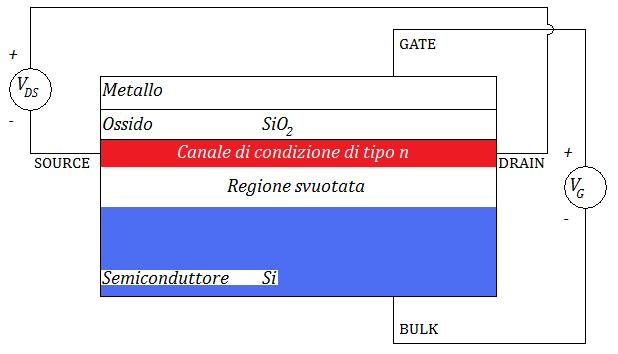
\includegraphics[scale=0.45]{119.png}
			\caption{Un transistore MOSFET. Si noti che la corrente di gate $I_G$ è certamente nulla grazie alla presenza dell'isolante.}
			\label{fig:im-119}
		\end{figure}
	\end{center}
	Anche questo sistema è però piuttosto complesso da realizzare in dimensioni ridotte.\\
	Sfruttiamo allora la versione di Figura \ref{fig:im-120} che è più facile da gestire.
	\begin{center}
		\begin{figure}[h]
			\centering
			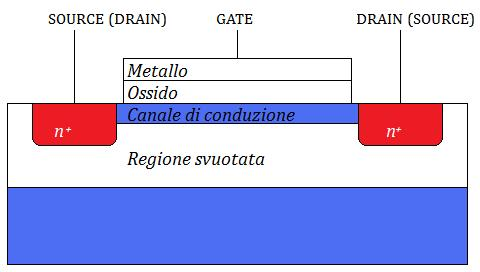
\includegraphics[scale=0.45]{120.png}
			\caption{Un transistore MOSFET realizzato su un pezzo di semiconduttore. \\ La regione svuotata circonda completamente il dispositivo.}
			\label{fig:im-120}
		\end{figure}
	\end{center}
	Tale dispositivo presenta due enormi vantaggi: l'intera struttura di conduzione, facilmente realizzabile, “galleggia” in una zona completamente neutra (non abbiamo quindi bisogno di complesse strutture di isolamento) e la corrente di gate è intrinsecamente nulla.\\
	Un altro indubbio vantaggio del MOSFET è che, contrariamente al BJT, si tratta di un dispositivo completamente simmetrico e quindi possiamo scambiare il drain ed il source senza problemi.
	\subsubsection{Analisi quantitativa}
	Abbiamo ormai compreso che il MOSFET è un dispositivo estremamente utile ed interessante.\\
	Passiamo all'analisi quantitativa considerando lo schema di Figura \ref{fig:im-121}.\\\\
	Ipotizziamo che l'ossido abbia una dimensione pari a $T_{OX}$ e che esista una coordinata $x_D$ oltre la quale l'interfaccia tra ossido e semiconduttore non abbia più effetto.
	\begin{center}
		\begin{figure}[h]
			\centering
			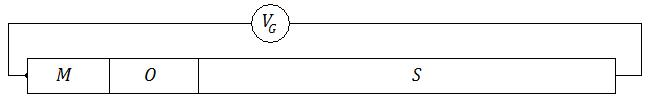
\includegraphics[scale=0.45]{121.png}
			\caption{Schema semplificato di un transistore MOSFET.}
			\label{fig:im-121}
		\end{figure}
	\end{center}
	\paragraph{Condizione per $x > x_D$}
	Incominciamo l'analisi partendo dalla regione svuotata.\\
	Per ipotesi in questa regione è:
	$$\begin{cases} p = p_0 = N_A \\ n = n_0 = \frac{n^2}{N_A} \end{cases}$$
	da cui ricaviamo che il campo elettrico è:
	$$E = -qD_p \frac{dp}{dx} = 0$$
	Inoltre, siccome il potenziale $\varphi$ è definito a meno di una costante possiamo imporre che sia $\varphi = 0$.\\\\
	Da ultimo anche la densità di carica $\rho$ è nulla.
	\paragraph{Condizione per $x < -T_{OX}$}
	Il potenziale $\varphi$ è nuovamente costante.\\
	Grazie a Kirchhoff ricaviamo:
	$$\varphi = V_G - \varphi_{MS} = V_G'$$
	dove $\varphi_{MS}$ è il potenziale di contatto tra metallo e semiconduttore.\\\\
	Siccome $\varphi$ è costante, il campo elettrico, che ne è la derivata, è nullo.
	\paragraph{Condizione per $-T_{OX} < x < 0$}
	Siamo nell'ossido.\\
	Supponiamo che l'ossido sia puro e quindi risulti:
	$$\rho = 0$$
	$$\begin{cases} \frac{d(\varepsilon E)}{dx} = \rho \\ \varepsilon = \varepsilon_{OX} \end{cases} \implies \frac{dE}{dx} = \frac{\rho}{\varepsilon} = 0$$
	ed allora sarà:
	$$E = E_{OX}$$
	Per quanto riguarda il potenziale, sfruttanddot quanto ricavato ed integrando, abbiamo:
	$$\varphi(x) = V_G' - E_{OX} \cdot (x + T_{OX})$$
	che è l'equazione di una retta a pendenza negativa.\\
	Il limite estremo è:
	$$\varphi_S = \varphi(0) = V_G' - E_{OX}T_{OX}$$
	Il campo elettrico alla superficie è allora:
	$$E_{OX} = \frac{V_G' - \varphi_S}{T_{OX}}$$
	\paragraph{Condizione per $0 < x < x_D$}
	Siamo nella regione perturbata.\\
	Ragionevolmente il potenziale $\varphi$ sarà compreso tra $\varphi_S$ (che è positivo) e $0$.
	$$\varphi_S > \varphi > \varphi(x_D)$$
	Inoltre nell'intervallo possiamo scrivere $\rho$ nella forma:
	$$\rho = (N_D - N_A + p - n)$$
	ma siccome $N_D$ non è fisicamente presente nel dispositivo, $p$ è trascurabile e $n \ll n_S \approx N_A$ è anch'esso trascurabile, abbiamo:
	$$\rho = -qN_A$$
	Allora sia il campo sia la densità di carica hanno un andamento rispettivamente di tipo lineare e di tipo parabolico come già visto per il diodo.
	\paragraph{Grafici riassuntivi}
	I grafici di Figura \ref{fig:im-122} mostrano le grandezze fondamentali di un transistore MOSFET.
	\begin{center}
		\begin{figure}[h]
			\centering
			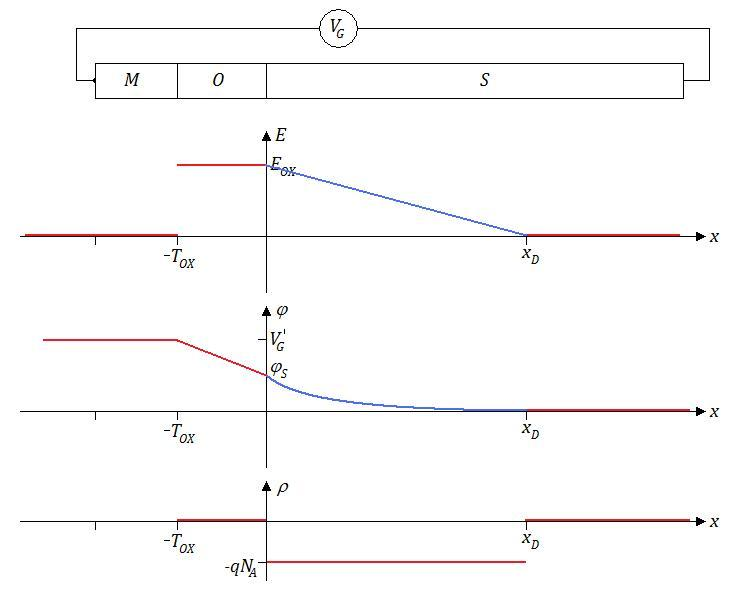
\includegraphics[scale=0.45]{122.png}
			\caption{Grandezze fondamentali di un transistore MOSFET. \\ In azzurro le porzioni di caratteristica che abbiamo solo ipotizzato.}
			\label{fig:im-122}
		\end{figure}
	\end{center}
	I risultati già ottenuti sono riportati in Figura \ref{fig:im-122}.\\\\
	In particolare ricordiamo che:
	$$x > x_D \Longrightarrow \begin{cases} E = 0 \\ \varphi = 0 \\ \rho = 0 \end{cases}$$
	$$x < -T_{OX} \Longrightarrow \begin{cases} E = 0 \\ \varphi = V'_G \end{cases}$$
	$$-T_{OX} < x < 0 \Longrightarrow \begin{cases} E = E_{OX} \\ \varphi = V'_G - E_{OX} \cdot (x + T_{OX}) \\ \rho = 0 \end{cases}$$
	Osserviamo che nel passaggio dalla regione di ossido alla regione di semiconduttore il campo elettrico non è continuo.\\
	Infatti è:
	$$\frac{dE}{dx} = \frac{\rho}{\varepsilon} = \frac{-qN_A}{\varepsilon_p}$$
	$$\int_{o^{-}}^{0^{+}} d(\varepsilon E) = \int_{o^{-}}^{0^{+}} \rho dx \Longrightarrow \varepsilon_{s} E_{s} - \varepsilon_{OX} E_{OX} = 0 \Longrightarrow \varepsilon_{s} E_{s} = \varepsilon_{OX} E_{OX}$$
	Allora il campo elettrico nel semiconduttore è:
	$$E_{s} = \frac{\varepsilon_{OX}}{\varepsilon_{s}} E_{OX}$$
	$$\frac{dE}{dx} = \frac{-qN_{A}}{\varepsilon_{s}} \Longrightarrow E(x) = \frac{qN_{A}}{\varepsilon_{s}} (x_{D} - x)$$
	Possiamo ora ricavare $\varphi$:
	$$\varphi(x) = \frac{qN_{A}}{2\varepsilon_{s}} (x - x_{D})^{2}$$
	$$0 < x < x_{D} \Longrightarrow \begin{cases} E(x) = \frac{qN_{A}}{\varepsilon_{s}} (x_{D} - x) \\ \varphi(x) = \frac{qN_{A}}{2\varepsilon_{s}} (x - x_{D})^{2} \\ \rho = -qN_{A} \end{cases}$$
	A questo punto è possibile ricavare il valore di $x_{D}$.
	$$\begin{cases} E(x) = \frac{qN_{A}}{\varepsilon_{s}} (x_{D} - x) \\ \varphi(x) = \frac{qN_{A}}{2\varepsilon_{s}} (x - x_{D})^{2} \end{cases} \quad \stackrel{x=0}{\Longrightarrow} x_{D} = \sqrt{\frac{2\varepsilon_{s}\varphi_{s}}{qN_{A}}}$$
	Con valori significativi risulta che l'ampiezza della zona perturbata (anche nel caso peggiore $\varphi_{s} = V'_{G}$) si misura in micron.\\
	Dunque l'ipotesi iniziale è verificata e possiamo fare altri ragionamenti.
	\subsection{Analisi della tensione $V'_{G}$}
	Nel semiconduttore avremo una carica di elettroni fortemente superficiale dovuta ai portatori mobili.\\
	Il grafico di Figura \ref{fig:im-123} mostra le due cariche della regione di semiconduttore.
	\begin{center}
		\begin{figure}[h]
			\centering
			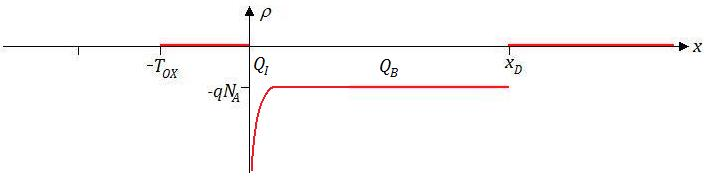
\includegraphics[scale=0.45]{123.png}
			\caption{La regione di semiconduttore presenta sia una carica superficiale ($Q_{i}$) sia una carica "profonda" ($Q_{B}$).}
			\label{fig:im-123}
		\end{figure}
	\end{center}
	La carica $Q_{B}$ è una carica fissa e si trova distribuita sotto la superficie del semiconduttore fino a punto $x_{D}$.\\
	La carica $Q_{I}$ è invece dovuta alle cariche mobili raggruppate all'interfaccia ossido semiconduttore.\\
	Dobbiamo ora trovare un modo per legare le due cariche (che vanno tenute distinte) alla variabile $V_{G}$ e non alla variabile $\varphi_{s}$.
	$$\rho = q(N_{D} - N_{A} + p - n)$$
	$$\begin{cases} N_{D} = 0 \\ p = p_{0} e^{-\frac{q\varphi_{s}}{KT}} \\ p_{0} = N_{A} \\ n = n_{0} e^{\frac{q\varphi_{s}}{KT}} \\ n_{0} = \frac{n_{1}^{2}}{N_{A}} \end{cases} \quad \Longrightarrow \rho = q\left(-N_{A} + N_{A} e^{-\frac{q\varphi_{s}}{KT}} - \frac{n_{1}^{2}}{N_{A}} e^{\frac{q\varphi_{s}}{KT}}\right)$$
	Sfruttando ora l’equazione di Poisson e mettendola a sistema con l’espressione di $\rho$:
	$$\frac{dE}{dx} = -\frac{d^2\varphi}{dx^2} = \frac{\rho}{\varepsilon_p}$$
	ricaviamo l’andamento riportato in Figura 24.3.
	\begin{center}
		\begin{figure}[h]
			\centering
			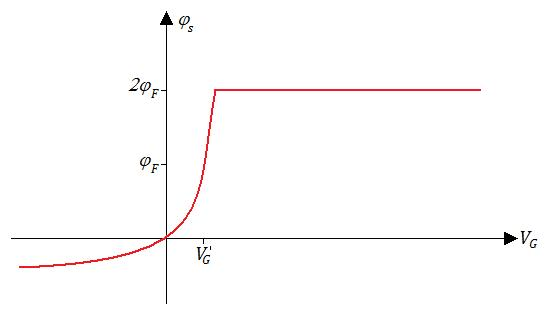
\includegraphics[scale=0.45]{124.png}
			\caption{Andamento di $\varphi_s$ al variare di $V_G$.}
			\label{fig:im-124}
		\end{figure}
	\end{center}
	Allora possiamo suddividere la curva in tre tratti: due a pendenza quasi nulla (per $V'_G < 0$ e per $V'_G > V^*_G$) ed uno ad elevata pendenza.
	\subsubsection{$V'_G$ = 0}
	Dal grafico ricaviamo che quando è:
	$$V'_G = 0 \implies \begin{cases} \varphi_s = 0 \\ n_s = n_0 \\ p_s = p_0 \end{cases}$$
	il potenziale è nullo nell’intera struttura.\\
	Inoltre le lacune e gli elettroni presentano la stessa concentrazione sia nel substrato sia nello strato di interfaccia.\\
	Questa situazione, detta di \textbf{banda piatta} (\textbf{flat band}), si ha solo quando risulta:
	$$V'_G = V_G - \psi_{MS} = 0 \implies V_G = \psi_{MS} = V_{FB}$$
	\subsubsection{$V'_G < 0$}
	In questa situazione abbiamo che il campo elettrico viene ribaltato: nel semiconduttore le lacune sono spinte verso la superficie mentre gli elettroni vengono spinti in profondità.
	$$V'_G < 0 \implies \begin{cases} \varphi_s < 0 \\ n_s < n_0 \\ p_s > p_0 \end{cases}$$
	Questa condizione, detta \textbf{condizione di accumulazione} poiché accumula i portatori maggioritari all’interfaccia,
	\subsubsection{$V'_G > 0$}
	In questa situazione abbiamo:
	$$V'_G > 0 \implies \begin{cases} \varphi_s > 0 \\ n_s > n_0 \\ p_s < p_0 \end{cases}$$
	e cioè un aumento della concentrazione di elettroni ed una diminuzione della concentrazione delle lacune.\\
	Dal grafico di Figura \ref{fig:im-124} notiamo che per $\varphi_s > \varphi_s^*$ gli elettroni e le lacune, alla superficie, si scambiano di ruolo: i portatori maggioritari divengono minoritari mentre i portatori minoritari divengono maggioritari.
	\begin{center}
		\begin{figure}[h]
			\centering
			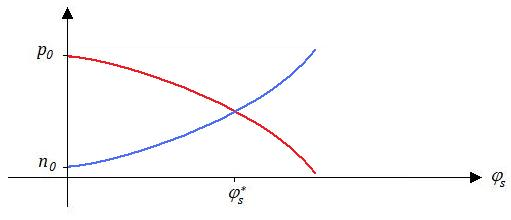
\includegraphics[scale=0.45]{125.png}
			\caption{Andamento della concentrazione superficiale di elettroni e di lacune.}
			\label{fig:im-125}
		\end{figure}
	\end{center}
	Questa condizione è detta di \textbf{inversione}.\\
	Il punto di inversione si ricava facilmente valutando l'uguaglianza:
	$$n_s(\varphi_s^*) = p_s(\varphi_s^*)$$
	Sfruttando le formule note ricordate all'inizio dell'analisi ricaviamo che è:
	$$\varphi_s^* = \frac{KT}{q} \cdot \ln\left[\frac{N_A}{n_i}\right]$$
	Il potenziale appena ricavato (note le concentrazioni di drogante è un numero) è detto \textbf{potenziale di Fermi} e viene indicato con $\varphi_F$.\\\\
	Possiamo allora distinguere due sottoregioni:
	\begin{itemize}
		\item una regione di \textbf{svuotamento }in cui è:
		$$\begin{cases} 0 < \varphi_s < \varphi_F \\ n_s < n_0 < p_s < p_0 \end{cases}$$
		\item una regione di \textbf{debole inversione} in cui è:
		$$\begin{cases} \varphi_s > \varphi_F \\ n_0 < p_s < n_s < p_0 \end{cases}$$
	\end{itemize}
	Inoltre per un certo valore di $\varphi_s$ la concentrazione degli elettroni alla superficie non supererà anche il valore assoluto delle lacune nel substrato.\\
	Per individuare tale valore di $\varphi_s$ sarà sufficiente imporre l'uguaglianza:
	$$n_s(\varphi_s^*) = p_0$$
	Anche in questo caso, sostituendo e semplificando ricaviamo che è:
	$$\varphi_s^* = 2 \cdot \frac{KT}{q} \cdot \ln\left[\frac{N_A}{n_i}\right] = 2\varphi_F$$
	Per distinguere la regione di inversione precedentemente ricavata da quella appena individuata diremo che per:
	$$\varphi_F < \varphi_s < 2\varphi_F$$
	ci troviamo in \textbf{debole inversione (weak inversion)} mentre per:
	$$\varphi_s > 2\varphi_F$$
	ci troviamo in \textbf{forte inversione (strong inversion)}.
	\subsubsection{Tabella riassuntiva e considerazioni}
	La Tabelle \ref{tab:table-13} riassume le regioni appena analizzate in relazione al potenziale superficiale $\varphi_s$.
	\begin{table}[h]
		\centering
		\begin{tabular}{ll}
			\hline
			$\varphi_s$ & Regione \\
			\hline
			$\varphi_s < 0$ & di accumulazione \\
			$0 < \varphi_s < \varphi_F$ & di svuotamento \\
			$\varphi_F < \varphi_s < 2\varphi_F$ & di debole inversione \\
			$\varphi_s > 2\varphi_F$ & di forte inversione \\
			\hline
		\end{tabular}
		\caption{Tabella riassuntiva delle regioni di $\varphi_s$.}
		\label{tab:table-13}
	\end{table}
	Possiamo inoltre associare il valore di $V_G'$ alle cariche $Q_B$ e $Q_I$.
	$$Q_B = -\sqrt{2qN_A\varepsilon_s\varphi_s}$$
	$$Q_I = C_{OX} \left( V_G' - V_G'^* \right)$$
	$$C_{OX} = \frac{\varepsilon_{OX}}{T_{OX}}$$
	L'andamento delle cariche in relazione a $V_G'$ è graficato in Figura \ref{fig:im-126}.\\\\
	Si noti che, oltre il punto $V_G^*$ (cioè in zona di forte inversione), l'aumento della carica dipende solamente dal valore di $Q_I$.
	\begin{center}
		\begin{figure}[h]
			\centering
			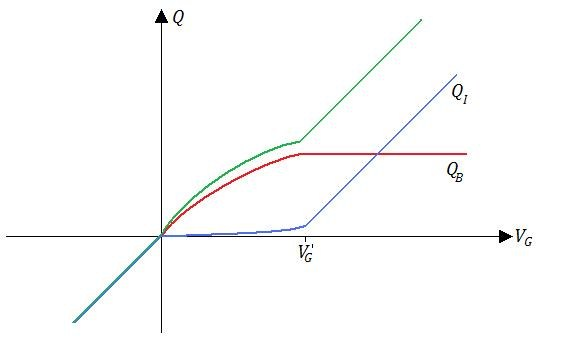
\includegraphics[scale=0.45]{126.png}
			\caption{Andamento della carica $Q$. \\ Si noti che essa è composta dalla somma della carica $Q_I$ e della carica $Q_B$.}
			\label{fig:im-126}
		\end{figure}
	\end{center}
	\subsection{Capacità del MOS}
	Abbiamo appena analizzato la distribuzione di carica all'interno di un condensatore MOS.\\
	I ragionamenti effettuati ci hanno portato a riconoscere quattro regioni: di accumulazione (che useremo molto di rado), di svuotamento, di debole inversione e di forte inversione.\\
	Abbiamo inoltre definito $Q_B$ come la \textbf{carica di bulk} e $Q_I$ come la \textbf{carica di interfaccia} e di inversione ed identificato
	$$x_D = \sqrt{\frac{2\varepsilon\psi_b}{qN_A}}$$
	Abbiamo infine notato che in regione di forte inversione il MOS risulta essere un normale condensatore.\\\\
	Partendo dal grafico della carica rispetto alla tensione del condensatore MOS possiamo ricavare la capacità equivalente del condensatore.
	$$C(V) = \frac{dQ}{dV}$$
	Possiamo definire la capacità massima del condensatore MOS come $C_{OX}$ in modo da, eventualmente, sovrastimare un ritardo.\\\\
	Ancora una volta siamo in presenza di un condensatore anomalo con capacità variabile (Figura \ref{fig:im-127}).
	\begin{center}
		\begin{figure}[h]
			\centering
			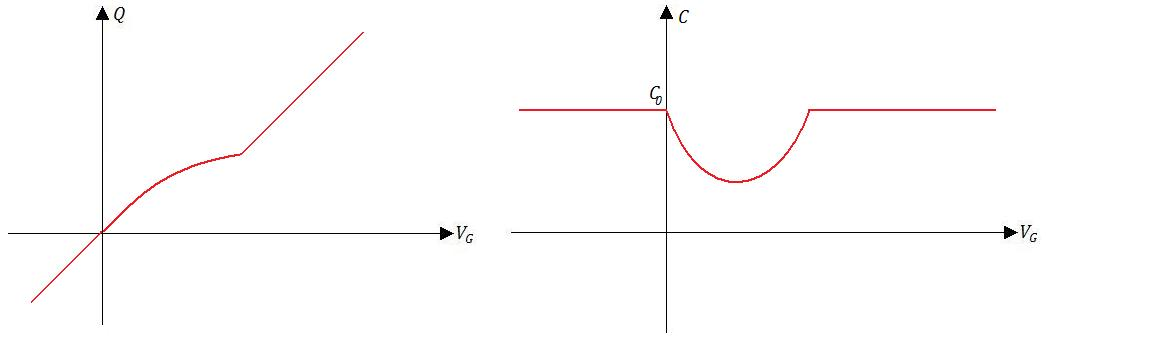
\includegraphics[scale=0.45]{127.png}
			\caption{Andamento qualitativo della carica $Q$ e della capacità ad essa associata.}
			\label{fig:im-127}
		\end{figure}
	\end{center}
%************************************************************************************************************************************************************************************
	\section{Tensione di soglia MOS}
	\subsection{Tensione di soglia}
	Notiamo che $V_G'^*$ discrimina due regioni: una in cui il canale esiste ed una in cui il canale ancora non esiste.\\
	Per questo motivo indichiamo questo valore con il nome di tensione di soglia ($V_T'$).
	$$V_T' = \left\{ V_G' : \varphi_s = 2\varphi_F \right\}$$
	Per calcolare il valore della tensione di soglia ricordiamo:
	$$E_{OX} = \frac{V'_G - \varphi_s}{T_{OX}}$$
	$$E_S = \frac{q N_A x_D}{\varepsilon_S}$$
	$$\varepsilon_{OX} E_{OX} = \varepsilon_S E_S$$
	da cui possiamo ricavare:
	$$\frac{\varepsilon_{OX}}{T_{OX}} \left( V'_T - 2\varphi_F \right) = \varepsilon_S \cdot \frac{q N_A}{\varepsilon_S} \cdot \sqrt{\frac{2\varepsilon_S}{q N_A}} \cdot \sqrt{2\varphi_F}$$
	$$V'_T = 2\varphi_F + \frac{\sqrt{2\varepsilon_S q N_A}}{C_{OX}} \cdot \sqrt{2\varphi_F}$$
	Siccome però noi controlliamo la tensione di soglia $V_T$ è più comodo esprimere:
	$$V'_T = V_T - \psi_{MS} \implies V_T = V'_T + \psi_{MS}$$
	Definendo ora:
	$$\frac{\sqrt{2\varepsilon_S q N_A}}{C_{OX}} = \gamma$$
	otteniamo l'espressione:
	$$V_T = \psi_{MS} + \gamma \cdot \sqrt{2\varphi_F} + 2\varphi_F$$
	che è nettamente più maneggevole.\\
	Inoltre $\psi_{MS}$ indica che deve essere pareggiato il potenziale di contatto tra metallo e semiconduttore, $\gamma \cdot \sqrt{2\varphi_F}$ indica che deve essere svuotato il bulk e $2\varphi_F$ indica il potenziale da raggiungere per entrare in forte inversione.\\\\
	Per abbassare od alzare la tensione di soglia è possibile drogare in modo opportuno lo strato superficiale (aggiungendo elettroni per abbassare $V_T$ od aggiungendo lacune per alzarne il valore).\\
	Solitamente queste modifiche si effettuano in fase di costruzione del dispositivo.\\\\
	Possiamo inoltre esprimere la carica di interfaccia come:
	$$Q_I = C_{OX} \cdot \left( V'_G - V'_T \right) \implies Q_I = C_{OX} \cdot (V_G - V_T)$$
%************************************************************************************************************************************************************************************
	\section{Transistore MOS, modello e caratteristiche parametriche}
	\subsection{Transistore MOS}
	Vediamo ora come applicare le relazioni trovate ad un transistore MOS (Figura \ref{fig:im-128})
	\begin{center}
		\begin{figure}[h]
			\centering
			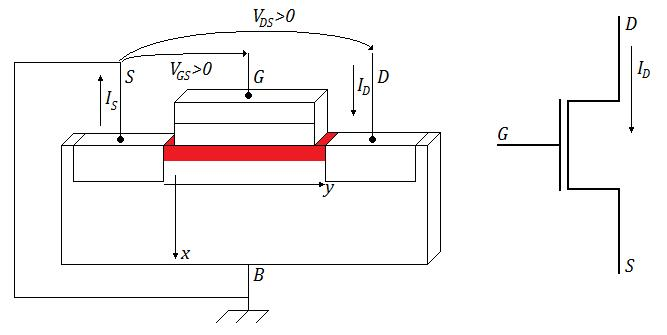
\includegraphics[scale=0.45]{128.png}
			\caption{Transistore MOS e suo simbolo circuitale. \\ Il canale di conduzione (evidenziato in rosso ha lunghezza $L$ e larghezza $W$).}
			\label{fig:im-128}
		\end{figure}
	\end{center}
	Una volta creato il canale di conduzione vogliamo trasferire corrente lungo l'asse $y$ dal source al drain.\\
	Sappiamo che sia la corrente di gate e la corrente di bulk sono nulle.\\
	Allora sarà:
	$$\begin{cases} I_G = 0 \\ I_B = 0 \\ I_D = -I_S \end{cases}$$
	Ipotizziamo di mettere a massa sia il bulk sia il source e di applicare una differenza di potenziale positiva $V_{DS}$ tra drain e source ed una differenza di potenziale positiva $V_{GS}$ tra gate e source.\\\\
	Vogliamo quindi individuare la corrente
	$$I_D(V_{GS}, V_{DS})$$
	Muovendoci lungo l'asse $y$ di Figura \ref{fig:im-128} notiamo che la tensione cresce dal valore 0 assunto in prossimità del source al valore $V_{DS}$ assunto in prossimità del drain.\\
	Allora la carica accumulata da ogni condensatore di dimensione $dy$ è funzione di $y$.
	$$Q_I(y) = C_{OX}(V_{GS} - \varphi(y) - V_T)$$
	Siccome siamo in una situazione bidimensionale il campo elettrico ha sempre due componenti.\\
	Semplifichiamo i calcoli supponendo di essere in una condizione di \textbf{profilo graduale} e cioè che il campo longitudinale abbia effetti trascurabili sul campo verticale e che il campo verticale non risenta delle variazioni del campo longitudinale.\\\\
	Per la convenzione scelta, la corrente $I_D$ scorre dal terminale di drain al terminale di source.
	$$I_D = -\int_s J ds$$
	dove $s$ indica una sezione infinitesima del dispositivo.\\
	Assumiamo che il canale sia di lunghezza $L$ e di larghezza $W$.\\
	Possiamo riscrivere:
	$$I_D = -W \int_0^{+\infty} J dx$$
	Siccome il canale è già completamente formato risulta essere:
	$$J = J_n = q\mu_n n E + qD_n \frac{dn}{dy}$$
	Dal momento che il canale è formato la componente diffusiva non conta (essendo derivata della concentrazione, che è costante, risulta essere nulla) ed allora semplifichiamo ulteriormente:
	$$J = q\mu_n n E$$
	$$I_D = -W \cdot \int_o^{+\infty} [q\mu_n n E_y] dx$$
	Osserviamo ora che $\mu_n$ è costante.\\
	Inoltre, essendo in ipotesi di profilo graduale, la componendo di campo $E_y$ è costante rispetto ad $x$.\\
	Allora è:
	$$I_D = -W \mu_n E_y \cdot \int_o^{+\infty} [qn] dx$$
	Il termine $n$ indica la concentrazione degli elettroni che varia lungo $x$ e non può essere estratto dall'integrale.\\
	Inoltre $qn$ è una densità di carica mobile che, integrata, porta alla carica di interfaccia.
	$$\int_0^{+\infty} [qn] \, dx = Q_I$$
	$$I_D = -\mu_n W C_{OX} (V_{GS} - V_T - \varphi(y)) E_y$$
	Ricordando ora che è sempre possibile scrivere:
	$$E_y = -\frac{d\varphi}{dy}$$
	otteniamo:
	$$I_D = \mu_n W C_{OX} (V_{GS} - V_T - \varphi(y)) \frac{d\varphi}{dy}$$
	Separiamo le variabili:
	$$I_D dy = \mu_n W C_{OX} (V_{GS} - V_T - \varphi(y)) \, d\varphi$$
	possiamo integrare ambo i membri:
	$$\int_0^L I_D dy = \int_{\varphi(0)}^{\varphi(L)} \mu_n W C_{OX} (V_{GS} - V_T - \varphi(y)) \, d\varphi$$
	$$I_D L = \mu_n W C_{OX} \left[ \left( V_{GS} - V_T\right) \varphi - \frac{\varphi^2}{2} \right]^{\varphi(L)}_{\varphi(0)}$$
	Ricordando ora che $\varphi(L) = V_{DS}$ e $\varphi(0) = 0$ otteniamo:
	$$I_D = \mu_n C_{OX} \cdot \frac{W}{L} \cdot \left[ (V_{GS} - V_T) V_{DS} - \frac{V_{DS}^2}{2} \right]$$
	che è valida fino a quando le ipotesi formulate sono valide.\\\\
	Vogliamo ora tracciare l'andamendo della corrente di drain in funzione della tensione $V_{DS}$ usando come parametro la tensione $V_{DS}$.\\\\
	Notiamo anzitutto che
	$$\mu_n C_{OX} \cdot \frac{W}{L} = \beta$$
	è costante.\\
	In particolare possiamo definire $\frac{W}{L}$ come il fattore di forma del canale.\\
	Dal momento che vogliamo tracciare curve a $V_{GS}$ costante dobbiamo analizzare la dipendenza di
	$$\left[ (V_{GS} - V_T) V_{DS} - \frac{V_{DS}^2}{2} \right]$$
	da $V_{GS}$.\\
	Possiamo suddividere il termine variabile in due componenti: una ($A = (V_{GS} - V_T) V_{DS}$) è una retta passante per l'origine e dipendente da $V_{GS}$; l'altra ($B = -\frac{V_{DS}^2}{2}$) è una parabola a concavità rivolta verso il basso ed indipendente da $V_{GS}$.\\\\
	Il profilo riportato in Figura \ref{fig:im-129} è il profilo che abbiamo nel caso siano verificate tutte le ipotesi ($V_{DS} > V_T$, di profilo graduale e di trasporto ohmico).\\\\
	Dai dati sperimentali notiamo che il modello così ottenuto è rispettato solamente fino al raggiungimento del massimo delle curve.\\
	Dal raggiungimento del massimo la corrente si mantiene costante (si noti l'analogia con la famiglia delle caratteristiche del BJT che consente di costruire gli stessi dispositivi in modo molto più semplice).\\\\
	Il massimo della curva ($V_{DS}^*$) è un punto importante poiché segna la differenza tra la parte ben descritta dal nostro modello approssimato e la parte dove il modello non funziona più.
	\begin{center}
		\begin{figure}[h]
			\centering
			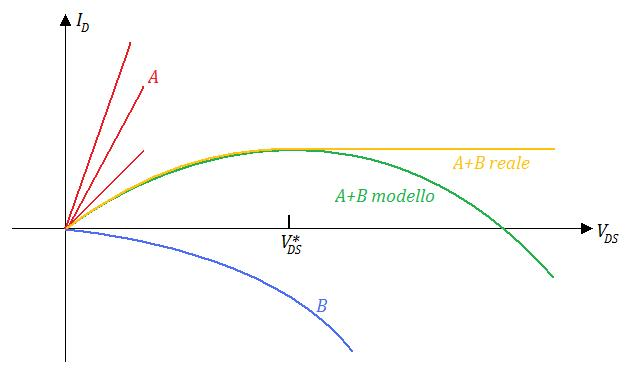
\includegraphics[scale=0.45]{129.png}
			\caption{Andamento qualitativo della corrente $I_D$ al variare di $V_{DS}$. \\ In rosso la componente identificata con $A$; in blu la componente $B$; in verde la somma $A + B$; in giallo il comportamento reale.}
			\label{fig:im-129}
		\end{figure}
	\end{center}
	$$\frac{dI_D}{dV_{DS}} = \beta \cdot [V_{GS} - V_T - V_{DS}^*] = 0 \implies V_{DS}^* = V_{GS} - V_T$$
	$$I_D(V_{DS}^*) = \frac{\beta}{2} \cdot (V_{GS} - V_T)^2$$
	Si nota che il punto $V_{DS}^*$ è il punto in cui la differenza tra la tensione di gate e la tensione di drain eguaglia la tensione di soglia.
	$$\begin{cases} V_{DS} < V_{DS}^* & V_G - V_D > V_T \\ V_{DS} = V_{DS}^* & V_G - V_D = V_T \\ V_{DS} > V_{DS}^* & V_G - V_D < V_T \end{cases}$$
	Allora dal punto $V_{DS}^*$ in poi la carica superficiale si annulla.\\
	Conseguentemente il canale non è più formato e l'ipotesi di trasporto esclusivamente ohmico cade.\\\\
	Per la conservazione della carica però il restringimento dal canale obbliga gli elettroni a muoversi più velocemente.\\
	Siccome inoltre è:
	$$v_n = \mu_n E_y$$
	il campo elettrico $E_y$ risulta estremamente elevato (teoricamente tendente ad infinito) e conseguentemente cade anche l'ipotesi di profilo graduale.\\\\
	Il punto $V_{DS} = V_{DS}^*$ in cui il canale si strozza origina la \textbf{condizione di pinch-off}.
	\begin{center}
		\begin{figure}[h]
			\centering
			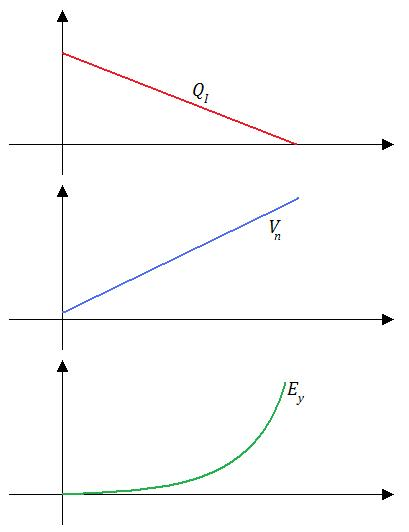
\includegraphics[scale=0.45]{130.png}
			\caption{Andamento qualitativo della velocità degli elettroni e del campo all'approssimarsi del punto di pinch-off.}
			\label{fig:im-130}
		\end{figure}
	\end{center}
%************************************************************************************************************************************************************************************
	\section{Invertitori nMOS ratioed (a carico resitivo, saturato, depletion, pseudo-nMOS)}
	\section{Invertitore CMOS}
	\section{Circuiti CMOS a più ingressi e funzione combinatoria arbitraria}
	\section{Composizione MOSFET in serie e parallelo}
	\section{Effetti reattivi MOSFET}
	\section{Tempi di propagazione invertitore CMOS}
	\section{Potenza invertitore CMOS}
	\section{Pass-transistor e Transmission gate}
	\section{Ritardo di propagazione lungo catene di pass-transistor (Elmore)}
	\section{Dimensionamento buffer CMOS}
	\section{Amplificatore operazionale ideale: principi e circuiti elementari}
	\section{OP-AMP: trigger e oscillatore}
	È un amplificatore operazionale con parte negativa connessa a terra.
%************************************************************************************************************************************************************************************
	\section{Conversione A/D}
	Un convertitore analogico-digitale (in inglese Analog to Digital Converter) è un circuito elettronico in grado di convertire un segnale analogico con andamento continuo (ad es. una tensione) in una serie di valori discreti (vedi teoria sulla conversione analogico-digitale).\\
	Il convertitore digitale-analogico o DAC compie l'operazione inversa. \\
	La maggior parte degli ADC sono lineari, il che significa che sono progettati per produrre in uscita un valore che è funzione lineare del segnale di ingresso. \\
	Un altro tipo comune di ADC è quello logaritmico, che è usato in sistemi di comunicazioni vocali per aumentare l'entropia del segnale digitalizzato. \\
	Il segnale analogico è tempo-continuo ed è necessario convertirlo in un flusso di valori discreti. \\
	È quindi necessario definire una frequenza alla quale campionare i valori discreti del segnale analogico. \\
	Questa frequenza è la frequenza di campionamento (sampling rate in inglese) del convertitore. \\
	L'idea chiave è che un segnale di banda limitata che varia con continuità può essere campionato e poi riprodotto esattamente dai valori tempo discreti con un algoritmo di interpolazione se la frequenza di campionamento è almeno pari al doppio della frequenza massima del segnale (teorema di Nyquist-Shannon).\\\\
	La precisione tuttavia è limitata dall'errore di quantizzazione. \\
	Poiché nella pratica un ADC non può effettuare una conversione istantanea, il valore d'ingresso deve necessariamente
	rimanere costante durante il tempo in cui il convertitore esegue la conversione (chiamato
	tempo di conversione o conversion time). \\
	Un circuito d'ingresso chiamato sample/hold svolge questo compito - spesso si usa un condensatore per immagazzinare la tensione del segnale in input e un interruttore elettronico per disconnettere il condensatore dall'ingresso.\\\\
	Molti ADC realizzati su circuiti integrati realizzano il sottosistema di sample/hold internamente.\\\\
	Per passare da D/A : Un singolo campione digitale è un numero, per trasformarlo in un segnale continuo è possibile associarvi un impulso rettangolare di altezza pari al suo valore e di durata predeterminata. \\
	Questa operazione detta Sample \& Hold che può essere eseguita in pratica con dispositivi elettronici, dal punto di vista matematico è una operazione di interpolazione che ha una sua ben precisa risposta in frequenza
	\section{Conversione D/A}
	Valgono gli stessi concetti della domanda precedente
	
\end{document}